% =====================================================================
%  MR2006B -- Autonomous Differential-Drive Vehicle
%  Technical Reference: hardware, physics, modelling, control,
%  estimation, lateral aiding, path planning, communication, open items
%
%  Build:   pdflatex MR2006B_Vehicle_Technical_Reference.tex   (run 3x)
%           or: latexmk -pdf MR2006B_Vehicle_Technical_Reference.tex
%  Images:  img/course_satellite.jpg, img/course_schematic.jpg
%           (both taken from "Challenge MR2006B.pdf"; the document still
%            compiles without them -- placeholders are drawn instead)
% =====================================================================
\documentclass[11pt,a4paper]{article}

\usepackage[T1]{fontenc}
\usepackage[utf8]{inputenc}
\usepackage[english]{babel}
\usepackage{mathpazo}
\usepackage[scaled=0.9]{helvet}
\renewcommand{\ttdefault}{txtt}
\usepackage{microtype}
\usepackage[a4paper,margin=24mm,bottom=27mm,headheight=14pt]{geometry}
\usepackage{xcolor}
\usepackage{graphicx}
\usepackage{booktabs}
\usepackage{tabularx}
\usepackage{longtable}
\usepackage{xltabular}
\usepackage{array}
\usepackage{multirow}
\usepackage{enumitem}
\usepackage{amsmath,amssymb,mathtools,bm}
\usepackage{siunitx}
\sisetup{per-mode=symbol,group-minimum-digits=5,detect-all,uncertainty-mode=separate}
\usepackage{titlesec}
\usepackage{fancyhdr}
\usepackage{caption}
\usepackage{float}
\usepackage{tikz}
\usepackage{pgfplots}
\pgfplotsset{compat=1.18}
\usetikzlibrary{positioning,arrows.meta,calc,fit,backgrounds,
                shapes.geometric,decorations.pathreplacing,patterns,
                decorations.markings}
\usepackage[most]{tcolorbox}
\usepackage[colorlinks=true,linkcolor=accent,urlcolor=accent,
            citecolor=accent]{hyperref}
\usepackage[nameinlink,capitalise]{cleveref}

% ---------------------------------------------------------------- colours
\definecolor{accent}{HTML}{B4522A}
\definecolor{accentbg}{HTML}{F5E6DE}
\definecolor{cold}{HTML}{3A5F7D}
\definecolor{coldbg}{HTML}{E2EBF2}
\definecolor{good}{HTML}{3F6B48}
\definecolor{goodbg}{HTML}{E4EFE6}
\definecolor{warn}{HTML}{9A6A13}
\definecolor{warnbg}{HTML}{F7EDD6}
\definecolor{bad}{HTML}{9B2D2D}
\definecolor{badbg}{HTML}{F6E1E1}
\definecolor{grey}{HTML}{7B776E}
\definecolor{greybg}{HTML}{F1EFEB}
\definecolor{rule}{HTML}{D8D4CC}

% ---------------------------------------------------------------- layout
\titleformat{\section}{\Large\bfseries\sffamily}{\color{accent}\thesection}{0.8em}{}
\titleformat{\subsection}{\large\bfseries\sffamily}{\thesubsection}{0.6em}{}
\titleformat{\subsubsection}{\normalsize\bfseries\sffamily}{\thesubsubsection}{0.6em}{}
\titlespacing*{\section}{0pt}{18pt}{6pt}
\titlespacing*{\subsection}{0pt}{12pt}{4pt}
\titlespacing*{\subsubsection}{0pt}{9pt}{3pt}
\setcounter{tocdepth}{2}
\setcounter{secnumdepth}{3}

\captionsetup{font=small,labelfont={bf,color=accent},width=0.94\textwidth}

\pagestyle{fancy}\fancyhf{}
\fancyhead[L]{\footnotesize\sffamily\color{grey}MR2006B \textperiodcentered{} Vehicle Technical Reference}
\fancyhead[R]{\footnotesize\sffamily\color{grey}Rev.\,1.0 \textperiodcentered{} 14 Oct 2026 \textperiodcentered{} week 6}
\fancyfoot[C]{\footnotesize\sffamily\color{grey}\thepage}
\renewcommand{\headrulewidth}{0.4pt}
\renewcommand{\headrule}{\hbox to\headwidth{\color{rule}\leaders\hrule height \headrulewidth\hfill}}

\setlength{\parindent}{0pt}
\setlength{\parskip}{5pt}
\setlist{itemsep=1pt,topsep=3pt}
\newcolumntype{L}{>{\raggedright\arraybackslash}X}
\newcolumntype{C}{>{\centering\arraybackslash}X}
\newcolumntype{P}[1]{>{\raggedright\arraybackslash}p{#1}}
\renewcommand{\arraystretch}{1.12}

% ---------------------------------------------------------------- boxes
\newtcolorbox{keybox}[1][]{enhanced,breakable,
  colback=accentbg,colframe=accent,boxrule=0pt,leftrule=2.5pt,
  arc=2pt,left=8pt,right=8pt,top=5pt,bottom=5pt,#1}
\newtcolorbox{warnbox}[1][]{enhanced,breakable,
  colback=warnbg,colframe=warn,boxrule=0pt,leftrule=2.5pt,
  arc=2pt,left=8pt,right=8pt,top=5pt,bottom=5pt,#1}
\newtcolorbox{goodbox}[1][]{enhanced,breakable,
  colback=goodbg,colframe=good,boxrule=0pt,leftrule=2.5pt,
  arc=2pt,left=8pt,right=8pt,top=5pt,bottom=5pt,#1}
\newtcolorbox{coldbox}[1][]{enhanced,breakable,
  colback=coldbg,colframe=cold,boxrule=0pt,leftrule=2.5pt,
  arc=2pt,left=8pt,right=8pt,top=5pt,bottom=5pt,#1}

% ---------------------------------------------------------------- markers
\newcommand{\mk}[2]{\textsf{\scriptsize\bfseries\colorbox{#1bg}{\color{#1}[#2]}}}
\newcommand{\MEASURE}{\mk{warn}{MEASURE}}
\newcommand{\VERIFY}{\mk{cold}{VERIFY}}
\newcommand{\DECIDE}{\mk{accent}{DECIDE}}
\newcommand{\ASK}{\mk{good}{ASK}}
\newcommand{\RISK}{\mk{bad}{RISK}}
\newcommand{\OPEN}{\mk{grey}{OPEN}}
\newcommand{\tg}[1]{{\small\textcolor{good}{\textsf{#1}}}}
\newcommand{\tw}[1]{{\small\textcolor{warn}{\textsf{#1}}}}
\newcommand{\tk}[1]{{\small\textcolor{cold}{\textsf{#1}}}}
\newcommand{\tb}[1]{{\small\textcolor{bad}{\textsf{#1}}}}
\newcommand{\code}[1]{\texttt{\small #1}}

% ---------------------------------------------------------------- maths
\newcommand{\sgn}{\operatorname{sgn}}
\newcommand{\sat}{\operatorname{sat}}
\newcommand{\diag}{\operatorname{diag}}
\newcommand{\E}{\operatorname{E}}
\newcommand{\dd}{\,\mathrm{d}}
\newcommand{\T}{^{\!\top}}
\newcommand{\vect}[1]{\bm{#1}}

% ---------------------------------------------------------------- TikZ
\tikzset{
  blk/.style   ={draw=rule,fill=greybg,rounded corners=3pt,
                 minimum height=9mm,align=center,font=\small\sffamily,inner sep=4pt},
  blkA/.style  ={blk,draw=accent,fill=accentbg},
  blkK/.style  ={blk,draw=cold,fill=coldbg},
  blkG/.style  ={blk,draw=good,fill=goodbg},
  blkW/.style  ={blk,draw=warn,fill=warnbg},
  blkB/.style  ={blk,draw=bad,fill=badbg},
  arr/.style   ={-{Latex[length=2.2mm]},draw=grey,thick},
  arrA/.style  ={-{Latex[length=2.2mm]},draw=accent,thick},
  arrK/.style  ={-{Latex[length=2.2mm]},draw=cold,thick},
  arrG/.style  ={-{Latex[length=2.2mm]},draw=good,thick},
  lbl/.style   ={font=\scriptsize\sffamily\color{grey}},
  rate/.style  ={font=\scriptsize\ttfamily\color{accent}},
  sum/.style   ={circle,draw=grey,thick,minimum size=5mm,inner sep=0pt,fill=white},
}
\pgfplotsset{
  mr/.style={axis line style={rule}, tick style={rule},
    label style={font=\small\color{grey}},
    tick label style={font=\scriptsize},
    legend style={font=\scriptsize,draw=rule},
    grid=major, grid style={rule,very thin}},
}

% safe image include: draws a placeholder if the file is missing
\newcommand{\safeimg}[2]{%
  \IfFileExists{#2}{\includegraphics[#1]{#2}}{%
    \fbox{\parbox[c][40mm][c]{0.8\textwidth}{\centering\small\color{grey}
      image #2 not found -- copy it from the source package}}}}
% =====================================================================
\begin{document}

\begin{titlepage}
\vspace*{22mm}
{\footnotesize\ttfamily\color{accent}MR2006B \textperiodcentered{} TECNOL\'OGICO DE MONTERREY \textperiodcentered{} AUTONOMOUS VEHICLE\par}
\vspace{5mm}
{\fontsize{30}{36}\selectfont\bfseries\sffamily Vehicle Technical Reference\par}
\vspace{5mm}
{\large\color{grey}Hardware, physical modelling, control, state estimation, lateral\\
aiding, path planning and communication of an STM32-controlled\\
differential-drive robot for the Jard\'in de las Carreras circuit\par}
\vspace{14mm}
{\color{rule}\rule{\textwidth}{0.4pt}}
\vspace{2mm}

\begin{tabularx}{\textwidth}{@{}>{\bfseries\sffamily\small}lL@{}}
Revision     & 1.0 --- 14 October 2026 (course week 6 of 16)\\
Platform     & NUCLEO-F446RE (STM32F446RET6, Cortex-M4F, \qty{180}{\mega\hertz}),
               differential drive, 2 driven wheels + 2 casters\\
Drivetrain   & 2\,$\times$\,JGB37-3530 / HS5141-178 (12\,V, 178\,rpm, 56.3:1, Hall encoder),
               2\,$\times$\,BTS7960 half-bridge modules\\
Status       & Drivetrain closed-loop on 50\,Hz cascade, radio link running,
               bench and wheels-in-air identification complete; IMU, ground sensors,
               EKF, path follower and mission logic still ahead\\
Sources      & \code{CONCEPT.md} Rev.\,F changeset, \code{BENCH\_README.md},
               \code{CALIB\_README.md}, \code{MR2006B\_CubeMX\_Konfiguration.xlsx}
               (09.10.2026), challenge brief \emph{Challenge MR2006B.pdf},
               design sessions weeks 1--6\\
Supersedes   & \emph{The Control System} overview (Rev.\,F, week 5)\\
\end{tabularx}

\vspace{2mm}
{\color{rule}\rule{\textwidth}{0.4pt}}

\vfill
\begin{coldbox}
\small\textbf{How to read this document.} Every number is labelled by its origin.
\emph{Measured} values carry the date and set-up of the measurement;
\emph{catalogue} values are marked as such; \emph{design} values are targets that
have not been verified on hardware. Open work is tagged inline, using the same
markers as \code{CONCEPT.md}:\\[1mm]
\MEASURE\ a quantity that must be measured \quad
\VERIFY\ a value that exists but is not yet confirmed \quad
\DECIDE\ a team decision \quad
\ASK\ a question for the professor or a vendor \quad
\RISK\ a known failure mode \quad
\OPEN\ unimplemented.\\[1mm]
All open items are collected in \cref{sec:open} with priority, owner action and
the sections they block.
\end{coldbox}
\end{titlepage}

\tableofcontents
\clearpage

% =====================================================================
\section*{Summary}
\addcontentsline{toc}{section}{Summary}

The vehicle is a \qty{\approx 0.4}{m} long differential-drive robot with two
driven wheels on a common axle and two passive casters. It must drive a closed
circuit of roughly \qty{150}{m} on paved paths around a garden of the Jard\'in de
las Carreras, stop for \qty{10}{s} at three waypoints, avoid obstacles, never
touch grass, and return to its start --- autonomously, powered by its own
battery, and with an STM32 as the only computer on board. Speed is not graded;
\textbf{completion, waypoint accuracy, obstacle handling and STM32-only operation
are.}

The design follows from that rubric. Absolute positioning (RTK-GNSS) is excluded
because a base station counts as an external aid. The vehicle therefore navigates
by \textbf{dead reckoning that is continuously corrected by the environment}:
wheel encoders give distance, a gyroscope gives heading, and downward- and
sideways-looking time-of-flight sensors measure the grass/path boundary, benches
and posts. A five-state Extended Kalman Filter fuses these. A cascade of
controllers --- mission logic, path follower, per-wheel position and speed
control --- turns the estimate into motion.

\begin{center}
\small
\begin{tabularx}{\textwidth}{@{}lL@{}}
\toprule
\textbf{Subsystem} & \textbf{State on 14 Oct 2026}\\
\midrule
Drivetrain model & Linear model $u=K_v\omega+K_s$ confirmed on the bench ($R^2>0.999$);
first-order plant identified on the BTS7960 ($K=\qty{7.60}{(mm/s)/\percent}$, $\tau=\qty{50}{ms}$)\\
Wheel control & Per-wheel cascade (trapezoid profile $\to$ P position $\to$ FF + PI speed) at \qty{50}{Hz};
\code{D1000} ends at 999.5/1000.3\,mm (firmware) \\
Odometry & Effective rolling diameter calibrated (72.6\,mm with a common 3584 counts/rev);
per-wheel scale and wheelbase still to be calibrated (UMBmark)\\
Communication & HC-12 at 9600\,Bd running in parallel to the USB console\\
IMU & ICM-42688-P unobtainable; \textbf{Adafruit ISM330DHCX} selected, not yet integrated\\
Ground / boundary sensing & 5\,$\times$\,VL53L1X ordered: 4 planned on I2C1 (ground), 1 spare; not yet installed \OPEN\\
EKF, path follower, mission & designed, not implemented \OPEN\\
\bottomrule
\end{tabularx}
\end{center}

The three facts that most shape the remaining work are: (i) the \textbf{entry
heading error} at the start of a reference-free segment dominates the error
budget (\cref{sec:budget}); (ii) the course itself has \textbf{not yet been
measured}, which blocks wheel size, landmark map and error budget
(\cref{sec:open}); and (iii) the drivetrain is \textbf{not a matched pair} ---
the two motors differ by \qty{12}{\percent} in speed and \qty{20}{\percent} in
breakaway duty at equal command, which the per-wheel feedforward and closed loop
must and do absorb (\cref{sec:pairing}).

% =====================================================================
\clearpage
\section{Task and requirements}\label{sec:task}

\subsection{The challenge}

The brief of course MR2006B (Sensors \& Actuators / Microcontrollers) requires a
vehicle capable of autonomous navigation. The binding requirements, taken
verbatim in content from the brief, are:

\begin{enumerate}[label=R\arabic*,leftmargin=10mm]
\item The vehicle must be \textbf{four-wheeled}; steering may be Ackermann or differential.
\item Chassis, motors and drivers must be assembled by \textbf{week 5} and are reviewed by the professor.
\item At least \textbf{one control loop} must be implemented (e.g.\ speed or direction control) and must respond to a user-controlled reference.
\item The robot must \textbf{transfer data} (telemetry) to an external system.
\item It must operate in \textbf{Manual} mode (responds to speed/direction commands) and \textbf{Automatic} mode (follows a pre-programmed trajectory autonomously).
\item It must traverse the circuit and \textbf{return to the start}, stopping \textbf{\qty{10}{s} at each waypoint}; a circuit is valid only if all grass is avoided and the paths are used.
\item It must perform \textbf{simple obstacle avoidance}.
\item Time limit \textbf{\qty{15}{min}}; battery powered; good presentation (no dangling cables).
\end{enumerate}

\Cref{fig:course} shows the circuit. Start and finish (X) lie next to the
bell of the Jard\'in de las Carreras; the vehicle drives south-west to the first
waypoint, north along the western path to the second waypoint, east along the northern path past a
\textbf{step} (red) that runs alongside the path, to the third waypoint in the
north-east and diagonally back to X. A \textbf{barrier} (black) borders the path
south-east of X, next to a small building.

\begin{figure}[htbp]
\centering
\begin{minipage}[c]{0.56\textwidth}\centering
\safeimg{width=\linewidth}{img/course_satellite.jpg}
\end{minipage}\hfill
\begin{minipage}[c]{0.42\textwidth}\centering
\safeimg{width=\linewidth}{img/course_schematic.jpg}
\end{minipage}
\caption{The circuit as given in the challenge brief. Left: satellite view with
the course outline (yellow). Right: schematic with start/stop X, waypoints O,
grass lines (green), step (red) and barrier (black). Driving direction is
clockwise around the central green. Tree canopy covers most of the paths ---
one of the reasons GNSS was rejected even before the external-aid ruling.
\MEASURE\ No dimension of this course has been measured yet (\cref{sec:open-field}).}
\label{fig:course}
\end{figure}

\subsection{Grading and what it implies}

\begin{center}
\small
\begin{tabular}{@{}lcl@{\hspace{10mm}}cc@{}}
\toprule
\multicolumn{3}{@{}l}{\textbf{Final prototype criteria}} & \multicolumn{2}{c}{\textbf{Waypoint accuracy}}\\
\cmidrule(r){1-3}\cmidrule(l){4-5}
Criterion & Points & Notes & Error [cm] & Grade\\
\midrule
Complete the circuit alone        & n/s  & treated as all-or-nothing & 0--5     & 2.00\\
No external aids to the sensors   & n/s  & excludes RTK base       & 5--10    & 1.75\\
Accuracy at waypoints             & 2    & table right             & 10--20   & 1.50\\
Obstacle avoidance                & 2/1/0 & reroute / wait / none  & 20--40   & 1.25\\
STM32 only                        & 2/1/0 & alone / with other MCU & 40--80   & 1.00\\
Exposition                        & 10   &                         & 80--160  & 0.75\\
                                  &      &                         & 160--320 & 0.50\\
                                  &      &                         & 320--640 & 0.25\\
                                  &      &                         & $>640$   & 0\\
\bottomrule
\end{tabular}\\[1mm]
{\footnotesize\color{grey}n/s = points not stated in the brief. The brief marks the accuracy column with ** but does not resolve the footnote: whether the error is taken per waypoint, as a mean or as the worst case is open \ASK.}
\end{center}

The accuracy scale is \textbf{logarithmic}: every halving of the error buys
\num{0.25} points. Going from \qty{80}{cm} to \qty{20}{cm} earns as much as
going from \qty{20}{cm} to \qty{5}{cm}, but costs a fraction of the effort.
Completion and STM32-only operation are binary. The design consequences:

\begin{keybox}
\textbf{Design rules derived from the rubric.}
\begin{enumerate}[leftmargin=5mm]
\item \textbf{Reliability beats precision.} A completed circuit with every waypoint
in the \qtyrange{10}{20}{cm} bracket (1.5 of 2 points) is the target. Chasing
\qtyrange{0}{5}{cm} is a 0.5-point gain at disproportionate risk.
\item \textbf{Speed is free.} Stop-and-turn instead of arcs, slow approach,
\qty{10}{s} ZUPT windows --- all cost only time, of which there is a reserve
(\cref{sec:timebudget}).
\item \textbf{Every correction is optional.} \emph{No fix is the normal case, not
a fault case.} The vehicle must complete the circuit on dead reckoning alone; each
aiding source only improves it.
\item \textbf{Genuine rerouting}, not only waiting, earns the second obstacle
point; the corridor geometry makes this a 1-D problem (\cref{sec:evasion}).
\item \textbf{Only the STM32 decides.} Sensor modules with their own firmware
(VL53L1X, HC-12) are peripherals; no co-processor runs navigation code.
\ASK\ The HC-12 contains an STM8 as its radio controller --- to be confirmed
with the professor as acceptable (\cref{sec:open-questions}, Q10).
\end{enumerate}
\end{keybox}

\subsection{Milestones}

\begin{center}
\small
\begin{tabularx}{\textwidth}{@{}clLc@{}}
\toprule
\textbf{Week} & \textbf{Milestone (graded)} & \textbf{Acceptance criterion used internally} & \textbf{State}\\
\midrule
5  & Chassis, motor and driver built and working & drives straight and turns in place under command & \tg{done}\\
8  & Sensory system & IMU, encoders, ToF logged with timestamps, $<1\,\%$ dropped frames & \tw{IMU chosen}\\
10 & Comms (telemetry) & full state logged at 10\,Hz for 15\,min & \tw{CSV link runs}\\
14 & Comms (remote control) & manual mode, failsafe verified & \tk{planned}\\
15 & Autonomous behaviour & full circuit without obstacles, waypoints within 40\,cm & \tk{planned}\\
16 & Complete system & obstacles, waypoints within 20\,cm, static obstacle evaded & \tk{planned}\\
\bottomrule
\end{tabularx}
\end{center}

Internal milestones in between: velocity loop tuned (week 8, done early on the
50\,Hz cascade), EKF stationary and hand-pushed (week 10), UMBmark and Allan
variance (week 12), path following on a \qtyproduct{10x10}{m} rectangle
(week 13), full \code{-O2} competition build (week 13).
% =====================================================================
\clearpage
\section{System overview}\label{sec:overview}

\subsection{Architecture}

The system is a cascade of four control layers with a state estimator beside
them, all executed by one STM32F446RE without an operating system. Each layer
generates the setpoint for the one below it; the estimator tells every layer
where the vehicle is. \Cref{fig:signalflow} shows the signals.

\begin{figure}[htbp]
\centering
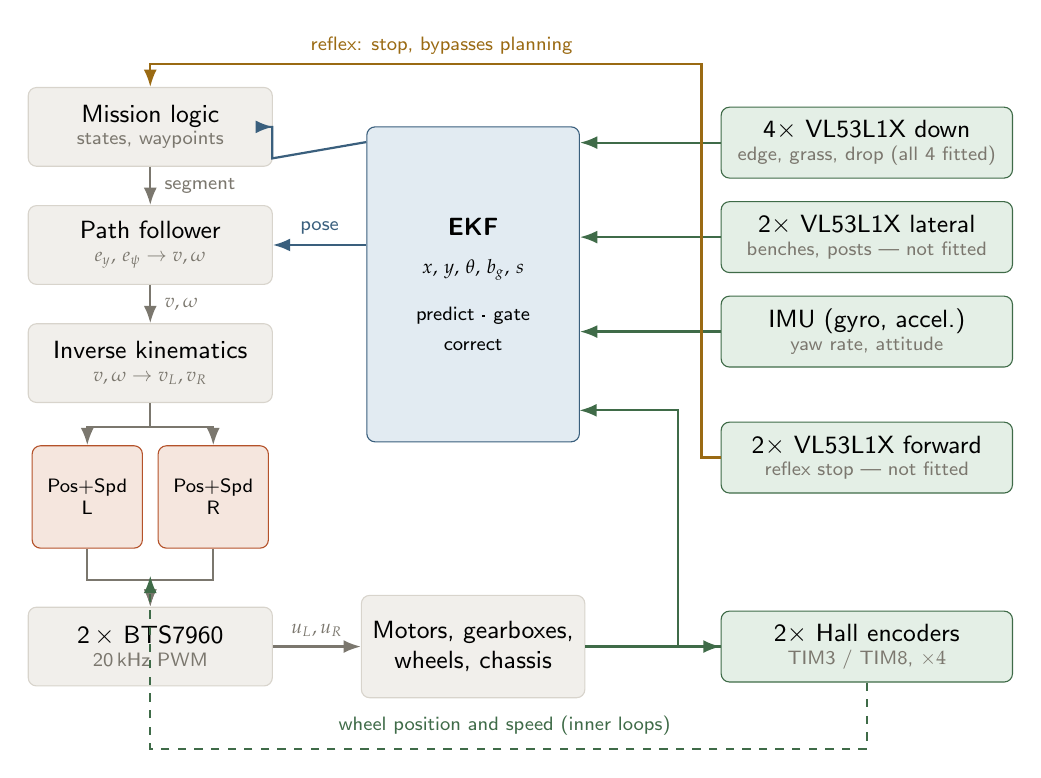
\begin{tikzpicture}[x=1cm,y=1cm]
  \tikzset{bx/.style={blk,minimum width=31mm,minimum height=10mm}}
  % left column: command path
  \node[bx]   (miss) at (1.9,10.2) {Mission logic\\[-1mm]{\scriptsize\color{grey}states, waypoints}};
  \node[bx]   (path) at (1.9,8.7)  {Path follower\\[-1mm]{\scriptsize\color{grey}$e_y,\,e_\psi \to v,\omega$}};
  \node[bx]   (kin)  at (1.9,7.2)  {Inverse kinematics\\[-1mm]{\scriptsize\color{grey}$v,\omega \to v_L,v_R$}};
  \node[blkA,minimum width=14mm,minimum height=13mm] (cl) at (1.1,5.5) {\scriptsize Pos+Spd\\[-1mm]\scriptsize L};
  \node[blkA,minimum width=14mm,minimum height=13mm] (cr) at (2.7,5.5) {\scriptsize Pos+Spd\\[-1mm]\scriptsize R};
  \node[bx]   (drv)  at (1.9,3.6)  {2\,$\times$ BTS7960\\[-1mm]{\scriptsize\color{grey}20\,kHz PWM}};
  % plant
  \node[blk,minimum width=27mm,minimum height=13mm] (plant) at (6.0,3.6)
       {Motors, gearboxes,\\wheels, chassis};
  % estimator
  \node[blkK,minimum width=27mm,minimum height=40mm] (ekf) at (6.0,8.2)
       {\textbf{EKF}\\[1mm]{\scriptsize $x,\,y,\,\theta,\,b_g,\,s$}\\[2mm]
        {\scriptsize predict \textperiodcentered{} gate}\\{\scriptsize correct}};
  % sensors
  \tikzset{sx/.style={blkG,minimum width=37mm,minimum height=9mm}}
  \node[sx] (vlg) at (11.0,10.0) {4$\times$ VL53L1X down\\[-1mm]{\scriptsize\color{grey}edge, grass, drop (all 4 fitted)}};
  \node[sx] (vll) at (11.0,8.8)  {2$\times$ VL53L1X lateral\\[-1mm]{\scriptsize\color{grey}benches, posts --- not fitted}};
  \node[sx] (imu) at (11.0,7.6)  {IMU (gyro, accel.)\\[-1mm]{\scriptsize\color{grey}yaw rate, attitude}};
  \node[sx] (vlf) at (11.0,6.0)  {2$\times$ VL53L1X forward\\[-1mm]{\scriptsize\color{grey}reflex stop --- not fitted}};
  \node[sx] (enc) at (11.0,3.6)  {2$\times$ Hall encoders\\[-1mm]{\scriptsize\color{grey}TIM3 / TIM8, $\times4$}};
  % arrows
  \draw[arr] (miss) -- (path) node[lbl,midway,right=0.5mm] {segment};
  \draw[arr] (path) -- (kin)  node[lbl,midway,right=0.5mm] {$v,\omega$};
  \draw[arr] (kin.south) -- ++(0,-0.3) -| (cl.north);
  \draw[arr] (kin.south) -- ++(0,-0.3) -| (cr.north);
  \draw[arr] (cl.south) -- ++(0,-0.4) -| (drv.north);
  \draw[arr] (cr.south) -- ++(0,-0.4) -| (drv.north);
  \draw[arr] (drv) -- (plant) node[lbl,midway,above] {$u_L,u_R$};
  \draw[arrG] (plant) -- (enc);
  \draw[arrG] (vlg.west) -- (ekf.east|-vlg.west);
  \draw[arrG] (vll.west) -- (ekf.east|-vll.west);
  \draw[arrG] (imu.west) -- (ekf.east|-imu.west);
  \draw[arrG] (enc.west) -- (8.6,3.6) -- (8.6,6.6) -- (7.35,6.6);
  \draw[draw=warn,thick,-{Latex[length=2.2mm]}] (vlf.west) -- (8.9,6.0) -- (8.9,11.0) -- (1.9,11.0) -- (miss.north);
  \node[lbl,text=warn,anchor=south] at (5.6,11.0) {reflex: stop, bypasses planning};
  \draw[arrK] (ekf.west|-path) -- (path.east) node[lbl,midway,above,text=cold] {pose};
  \draw[arrK] (ekf.north west) ++(0,-0.2) -- (3.45,9.8) -- (3.45,10.2) -- (miss.east);
  \draw[draw=good,dashed,thick,-{Latex[length=2.2mm]}] (enc.south) -- (11.0,2.3) -- (1.9,2.3) -- (1.9,4.5);
  \node[lbl,text=good,anchor=south] at (6.4,2.35) {wheel position and speed (inner loops)};
\end{tikzpicture}
\caption{Signal flow. Setpoints flow down the left, measurements return on the
right. The encoders feed two consumers: the wheel loops (fast, dashed) and the
EKF (distance increment). Heading rate comes from the gyroscope, \emph{not} from
the encoder difference, because the latter depends on the effective wheelbase,
which changes with every slip event. The forward sensors have a direct reflex
path that stops the vehicle without passing through the planner.}
\label{fig:signalflow}
\end{figure}

\subsection{Layers, rates and the present implementation}\label{sec:rates}

\begin{center}
\small
\begin{tabularx}{\textwidth}{@{}lccL@{}}
\toprule
\textbf{Layer} & \textbf{Concept rate} & \textbf{Implemented} & \textbf{Content}\\
\midrule
4 Mission logic       & 20\,Hz  & --- & state machine, waypoint sequencing, obstacle decisions\\
3 Path follower       & 100\,Hz & --- & cross-track/heading controller, TURN controller, speed profile\\
\multicolumn{1}{@{}l}{\quad Estimator (EKF)} & 200\,Hz & --- & prediction from encoder+gyro, corrections\\
2 Wheel control       & 200\,Hz (PI) & \textbf{50\,Hz} & trapezoid profile, P position, FF + PI speed, L/R sync\\
1 Actuation           & PWM     & \textbf{20\,kHz} & BTS7960 RPWM/LPWM, enable lines, slew limits\\
\bottomrule
\end{tabularx}
\end{center}

\begin{warnbox}
\textbf{Concept versus implementation --- deliberate deviation.} The concept
places the wheel PI at 200\,Hz in a 1\,kHz tick. The firmware on the vehicle
(teammate's \code{main.c}, extended 08--10 Oct) runs the whole wheel cascade at
\qty{50}{Hz} from TIM6. With velocity computed as a count difference, 50\,Hz is
the \emph{correct} choice: one count per sample is \qty{3.18}{mm/s} at 50\,Hz but
\qty{12.7}{mm/s} at 200\,Hz and \qty{63.6}{mm/s} at 1\,kHz (\cref{sec:encoder}).
Moving the loop faster requires a period-measurement (M/T) speed estimator first
(\cref{sec:opt}). Rule of thumb for the cascade: at least a factor of 5 between
adjacent loop bandwidths --- this, not the sample rate, constrains the path
follower (\cref{sec:pathfollow}).
\end{warnbox}

\subsection{Design principles}

These principles have decided every trade-off so far and are the
argumentation basis for the final defence.

\begin{enumerate}[leftmargin=6mm,label=P\arabic*]
\item \textbf{The rubric is the specification.} Speed optimisation and Ackermann steering were removed because they earn nothing.
\item \textbf{Observability first.} Ask \emph{which direction} a sensor constrains, not how well it sees (\cref{sec:observability}).
\item \textbf{No fix is the normal case.} Every aiding measurement is optional and gated.
\item \textbf{Prefer the observable failure.} A DC motor under overload slows down and the encoder sees it; a stepper loses steps silently. This rejected steppers, skid steer and GNSS fusion alike.
\item \textbf{Timestamps beat sample rate.} A 200\,Hz filter with exact $\Delta t$ beats a 1\,kHz filter with jitter. Hence no RTOS, a 1\,MHz free-running time base, and hardware input capture for data-ready edges.
\item \textbf{Commission one layer at a time.} Open loop before closed loop, bench before vehicle, stationary EKF before driving EKF.
\item \textbf{Measure the constant, do not inherit it.} $K_s$, $K_v$, gear ratio, wheel diameter, wheelbase are catalogue guesses until measured.
\item \textbf{Verify the delivered part, not the listing.} The PH2.0 connector, the BTS7960 input threshold and the H-bridge truth table all differed from or were undocumented in their listings.
\item \textbf{Structural safety over checks.} Forbidden driver states are made unreachable by construction (single setter), not tested for.
\end{enumerate}

\subsection{Rejected concepts}\label{sec:rejected}

\begin{center}
\small
\begin{tabularx}{\textwidth}{@{}lL@{}}
\toprule
\textbf{Rejected} & \textbf{Reason}\\
\midrule
RTK-GNSS / GNSS+IMU fusion & base station ruled an external aid by the professor; canopy multipath; GNSS modules contain their own processors\\
SLAM & corridor degeneracy (scan matching unconstrained along the path axis); the only loop closure comes after all waypoints are scored; a static-world assumption violated by moving robots; a \qty{10}{cm} grid of $40\times\qty{40}{m}$ already needs \qty{160}{KB} of the \qty{128}{KB} SRAM\\
Line-scan camera & illumination under canopy; no gain over geometric (height/reflectance) boundary detection\\
Ackermann steering & no turn in place; larger turning envelope at the ramp; nothing graded rewards it\\
NEMA 17 steppers & silent step loss (unobservable failure), poor torque at speed, current draw at standstill\\
Ultrasonic sensors (HC-SR04) & silent false negatives on oblique surfaces --- fatal in the reflex layer\\
Optical flow (PMW3901) & four independent grounds: (a) at \qty{0.4}{m/s}, 100\,fps and \qty{150}{mm} height only \num{1.2}\,px of motion per frame (20--30\,\% quantisation, an order coarser than the encoders); (b) wind-driven tree shadow is indistinguishable from translation --- a correlated phantom motion the EKF cannot reject; (c) it observes translation but not heading, the dominant error; (d) about two weeks of integration\\
Magnetometer heading & motor currents and structural steel distort the field ($\approx 8^\circ$ estimated near current-carrying wires)\\
FreeRTOS & context-switch jitter degrades $\Delta t$ in the EKF; harmonic cyclic executive suffices\\
TF-Luna LiDAR & cost; replaced by additional VL53L1X (one sensor type, one driver, no UART/DMA pressure)\\
C++ & ISR linkage pitfalls and hidden allocations; plain C with strict float discipline\\
\bottomrule
\end{tabularx}
\end{center}

The BTS7960 itself was first rejected (its 74AHC244 input buffer has
$V_{IH}=0.7\,V_{CC}$, i.e.\ \qty{3.5}{V} at 5\,V supply), then adopted once it was
recognised that powering the module's logic from \qty{3.3}{V} lowers the threshold
to $0.7\times3.3=\qty{2.31}{V}$, which the STM32's \qty{3.3}{V} outputs satisfy.
% =====================================================================
\clearpage
\section{Hardware}\label{sec:hardware}

\subsection{Bill of materials}\label{sec:bom}

Procurement is limited to local Mexican suppliers (Sandorobotics, MercadoLibre)
plus DigiKey/Mouser for parts without a local source. \Cref{tab:bom} lists every
component on or for the vehicle, with its status.

{\small
\begin{xltabular}{\textwidth}{@{}p{37mm}cL>{\raggedright\arraybackslash}p{24mm}@{}}
\caption{Complete hardware list. \emph{Status:} \tg{installed}, \tg{on hand},
\tw{to order}, \tk{decide}, \tb{blocked}.}\label{tab:bom}\\
\toprule
\textbf{Item} & \textbf{Qty} & \textbf{Specification / role} & \textbf{Status}\\
\midrule
\endfirsthead
\toprule
\textbf{Item} & \textbf{Qty} & \textbf{Specification / role} & \textbf{Status}\\
\midrule
\endhead
\bottomrule
\endfoot
\multicolumn{4}{@{}l}{\textbf{\textsf{Computing}}}\\
NUCLEO-F446RE & 1 & STM32F446RET6, LQFP64, Cortex-M4F with single-precision FPU, \qty{180}{MHz}, \qty{512}{KB} flash, \qty{128}{KB} SRAM; on-board ST-Link/V2-1 provides SWD, virtual COM port (USART2) and the \qty{8}{MHz} MCO clock used as HSE & \tg{installed}\newline \tw{spare advisable}\\
\midrule
\multicolumn{4}{@{}l}{\textbf{\textsf{Drivetrain}}}\\
Gear motor JGB37-3530 / HS5141-178 & 2 & \qty{12}{V} brushed DC, catalogue \qty{178}{rpm} no-load, gear ratio 56.3:1, \qty{3.4}{kgf.cm} (rated or stall: \ASK), stall current \qty{4.3}{A}; 6\,mm D-shaft & \tg{installed}\\
Hall quadrature encoder & 2 & integrated on the motor shaft, 16 PPR per channel, $\times4$ decoding $\Rightarrow$ 64 counts per motor revolution; open-collector outputs with $\approx\qty{3}{k\ohm}$ on-board pull-ups; supplied from \qty{3.3}{V} & \tg{installed}\\
BTS7960 module (IBT-2 / HW-039) & 2 & dual half-bridge (two BTS7960B), one module per motor; RPWM/LPWM inputs, R\_EN+L\_EN bridged; PWM up to \qty{25}{kHz}; logic VCC on \qty{3.3}{V} so that the 74AHC244 input threshold is $\approx\qty{2.3}{V}$ & \tg{installed}\\
Previous driver (bench) & 1 & opto-isolated dual H-bridge, L298-style EN+IN1+IN2 logic, $\leq\qty{10}{kHz}$ PWM; used for the week-5 bench constants; truth table measured & \tg{retired}\\
Hex adapter Pololu 2686 & 2 & \qty{6}{mm} D-shaft to \qty{12}{mm} hex, aluminium, \qty{20}{mm}; keeps the wheel choice open & \tg{installed}\\
Drive wheels & 2 & nominal \qty{76}{mm} (initial code value); effective rolling diameter \qty{72.6}{mm} calibrated with a common 3584 counts/rev & \tg{installed} \VERIFY\\
Casters & 2 & passive, size gated by the ramp-lip height & \tk{decide}\\
Motor brackets & 2 & JGB37 brackets & \tg{installed}\\
\midrule
\multicolumn{4}{@{}l}{\textbf{\textsf{Power}}}\\
LiPo 3S 2200\,mAh 35C & 1(+1) & \qtyrange{9.9}{12.6}{V}, \qty{11.1}{V} nominal; \qty{77}{A} short-circuit capability (fuse mandatory); second pack decided for 3-h sessions & \tg{1 on hand}\newline\tw{2nd to order}\\
B3 balance charger & 1 & balance charging only via the 4-pin JST-XH lead & \tg{on hand}\\
XT60 connector / pigtail, 14\,AWG & 2 & battery disconnect point & \tw{to order}\\
Fuse T10A (slow) + holder & 1 & main line; slow because a double stall draws \qty{8.6}{A} & \tw{to order}\\
Fuse F2--3A (fast) + holder & 1 & logic branch & \tw{to order}\\
Main switch $\geq\qty{10}{A}$ & 1 & before the star point, breaks both branches & \tw{to order}\\
Terminal block (star point) & 1 & only junction of motor and logic branches & \tw{to order}\\
Electrolytic \qtyrange{470}{1000}{\micro F}, \qty{25}{V} & 1 & bulk capacitor at the drivers & \tw{to order}\\
Ceramic \qty{100}{nF} & 6 & 3 per motor (terminal--terminal, each terminal--case), soldered before mounting & \tg{kit on hand}\\
Buck XY-3606, \qty{5}{V} fixed & 1 & logic supply, Nucleo via E5V; fixed output (no trimpot) & \tg{installed}\newline\VERIFY\ $U_{in,min}$\\
LDO AMS1117-3.3 & 1--2 & separate \qty{3.3}{V} sensor rail (keeps $V_{REF+}$ of the Nucleo clean) & \tg{installed}\newline\tb{overheated once}\\
Battery divider 47\,k$\Omega$/10\,k$\Omega$ & 1 & ratio $10/57=0.175$ to PA0 (ADC1) & \tw{to fit}\\
LiPo alarm, LiPo safety bag & 1+1 & independent cell monitor; charging safety & \tw{to order}\\
Wire 14--16\,AWG / 20\,AWG / 20--22\,AWG & --- & battery--drivers / motor leads (crimped) / logic & \tw{partly}\\
Standoffs & 1 set & driver underside can short & \tw{to order}\\
\midrule
\multicolumn{4}{@{}l}{\textbf{\textsf{Sensing}}}\\
VL53L1X ToF breakout & 5 & 4 fitted downward (ground/edge, I2C1), 1 spare; the 2 forward (reflex) and 2 lateral (benches, posts) positions are not covered \DECIDE; individual XSHUT for address assignment & \tw{ordered}\\
IMU (6-axis) & 1 & ICM-42688-P planned but unobtainable (0 stock, 16-week lead time); \textbf{Adafruit ISM330DHCX} selected; SPI + DMA, DRDY on input capture & \tw{to order/fit}\\
\midrule
\multicolumn{4}{@{}l}{\textbf{\textsf{Communication}}}\\
HC-12 radio (SI4463 based) & 2 & \qty{433}{MHz} band, transparent UART at \qty{9600}{Bd}, FU3, CH001; vehicle on USART1, ground station on FT232RL; SET on PC9 & \tg{running}\\
FT232RL USB--UART adapter & 1 & ground station side (Mac) & \tg{on hand}\\
\midrule
\multicolumn{4}{@{}l}{\textbf{\textsf{Development}}}\\
Lab supply, multimeter & --- & current-limited bring-up (\qty{6}{V}/\qty{100}{mA} truth-table test) & \tg{available}\\
Oscilloscope & --- & required for $U_{min}$ (driver output floor) and slot timing & \tw{access}\\
Mac + STM32CubeIDE 2.2 + CubeMX & --- & HAL-based C, Git in terminal & \tg{in use}\\
\end{xltabular}
}

\begin{warnbox}
\textbf{Few spares.} No spare motor, driver, Nucleo or IMU is on hand (one spare VL53L1X). One Nucleo
has already failed during the week-6 work (reported 10 Oct). A single defective
part now costs a week of lead time in a 16-week schedule. \RISK\ Recommended:
one spare Nucleo, one spare BTS7960 module, one spare motor.
\end{warnbox}

% ---------------------------------------------------------------------
\subsection{Microcontroller resources}\label{sec:mcu}

\subsubsection{Clock tree}\label{sec:clock}

The NUCLEO-F446RE has no crystal at X3. The \qty{8}{MHz} comes from the
ST-Link's MCO output, which is a clock \emph{signal} and therefore needs HSE in
\textbf{BYPASS} mode.

\begin{center}
\small
\begin{tabularx}{\textwidth}{@{}llL@{}}
\toprule
\textbf{Setting} & \textbf{Value} & \textbf{Reason}\\
\midrule
HSE & BYPASS, \qty{8}{MHz} & MCO is a square-wave signal; PH1 stays free. Crystal mode ``works'' by overdriving the oscillator amplifier --- marginal, not used\\
PLL source / M / N / P & HSE / 4 / 180 / 2 & VCO input $8/4=\qty{2}{MHz}$ (ST's recommendation for minimum jitter) $\to$ \qty{360}{MHz} VCO $\to$ \qty{180}{MHz}\\
AHB / APB1 / APB2 & /1 / /4 / /2 & HCLK 180, PCLK1 45 (timer clock \textbf{90}), PCLK2 90 (timer clock \textbf{180}) \si{MHz}\\
Voltage scale, over-drive, flash & VOS1, on, 5 WS & required at \qty{180}{MHz}; set automatically by CubeMX\\
LSE / LSI & off / on & no RTC; LSI for the IWDG\\
CSS & off (target: on) & needs \code{HAL\_RCC\_CSSCallback} that pulls EN\_L/EN\_R low first \OPEN\\
HSE start-up timeout & target \qty{1000}{ms} & default \qty{100}{ms} risks a failed start at power-on \VERIFY\\
\bottomrule
\end{tabularx}
\end{center}

\textbf{Why not HSI.} The internal RC oscillator is specified to
$\pm\qty{1}{\percent}$ over \qtyrange{0}{85}{\celsius}; the MCO derives from the
ST-Link crystal ($\approx\pm\qty{30}{ppm}$). A \qty{1}{\percent} clock error is a
\emph{scale error on every timestamp} and therefore on every integrated
quantity --- speed, gyro integration, ZUPT averaging --- and it is
temperature-dependent. A PLLM error of /8 instead of /4 already halved every bus
clock once (8 Oct) and made distance commands run at the wrong rate; the clock
tree is therefore verified in generated code after every regeneration.

\begin{warnbox}
\textbf{Battery operation without USB.} \RISK\ HSE BYPASS depends on the
ST-Link MCO. Whether the ST-Link section is powered and outputs MCO when the
board is supplied through E5V only, without USB, is untested \VERIFY. If it is
not, the clock start fails and \code{Error\_Handler} is entered. Mitigations in
order: (1) test E5V-only start; (2) USB power bank on the ST-Link connector; (3)
fit an \qty{8}{MHz} crystal at X3 (with C33/C34 and solder bridges per UM1724)
and switch HSE to crystal mode.
\end{warnbox}

\subsubsection{Timers}\label{sec:timers}

\begin{center}
\small
\begin{tabularx}{\textwidth}{@{}llrrrL@{}}
\toprule
\textbf{Timer} & \textbf{Function} & \textbf{Clock} & \textbf{PSC} & \textbf{ARR} & \textbf{Result / note}\\
\midrule
TIM1 & PWM CH1--4 (BTS7960) & 180\,MHz & 0 & 8999 & \qty{20}{kHz}, set at run time by \code{PWM\_Setup()}; 9000 steps = \qty{0.011}{\percent} resolution\\
TIM3 & encoder L (PA6/PA7) & 90\,MHz & 0 & 65535 & encoder mode TI1+TI2 ($\times4$), IC filter 15, CKD /1\\
TIM8 & encoder R (PC6/PC7) & 180\,MHz & 0 & 65535 & as TIM3, CKD /2 to equalise the filter time\\
TIM6 & control tick & 90\,MHz & 8999 & \textbf{199} & \qty{50}{Hz} $=1/\code{CTRL\_PERIOD\_S}$; last shared code had 119 $\Rightarrow$ \qty{83.3}{Hz} \tb{fix}\\
TIM2 & 32-bit time base, IC on PA1 & 90\,MHz & 0 $\to$ 89 & $2^{32}-1$ & target \qty{1}{MHz} (wrap \qty{71.6}{min}); IMU DRDY input capture \OPEN\\
SysTick & HAL time base & HCLK & --- & --- & must stay SysTick; TIM6 as HAL time base would collide with the control callback\\
\bottomrule
\end{tabularx}
\end{center}

\textbf{Encoder input filter.} Filter setting 15 samples 8 times at
$f_{DTS}/32$. TIM3: $f_{DTS}=\qty{90}{MHz}$ $\Rightarrow$
$8\cdot32/\qty{90}{MHz}=\qty{2.84}{\micro s}$; TIM8 with CKD/2 also
$f_{DTS}=\qty{90}{MHz}$ $\Rightarrow$ \qty{2.84}{\micro s}. Fastest edge spacing at
no-load (\cref{sec:encoder}) is \qty{92}{\micro s}: the filter consumes
\qty{3}{\percent} of it. With the encoders' \qty{3}{k\ohm} pull-ups and an
optional 1\,k$\Omega$/1\,nF RC the rise time is $\approx\qty{4}{\micro s}$ ---
still uncritical.

\subsubsection{Pin allocation}\label{sec:pins}

\begin{center}
\footnotesize
\begin{tabularx}{\textwidth}{@{}P{18mm}P{19mm}P{27mm}P{29mm}L@{}}
\toprule
\textbf{Pin} & \textbf{Morpho} & \textbf{Function} & \textbf{Target} & \textbf{Note}\\
\midrule
PA8 / PA9   & CN10-23 / -21 & TIM1\_CH1/CH2 & BTS7960 L RPWM / LPWM & forward / reverse\\
PA10 / PA11 & CN10-33 / -14 & TIM1\_CH3/CH4 & BTS7960 R RPWM / LPWM & \\
PB12 / PB13 & CN10-16 / -30 & GPIO out, pull-down & EN\_L / EN\_R (R\_EN+L\_EN) & plus external \qty{10}{k\ohm} to GND: defined off during reset\\
PA6 / PA7   & CN10-13 / -15 & TIM3\_CH1/CH2 & encoder L A / B & \\
PC6 / PC7   & CN10-4 / -19  & TIM8\_CH1/CH2 & encoder R A / B & TIM4 impossible: would remove USART1\\
PA2 / PA3   & internal      & USART2 & ST-Link VCP & 115200 Bd console\\
PB6 / PB7   & CN10-17 / CN7-21 & USART1 & HC-12 RXD / TXD & assign PB6/PB7 first, else CubeMX picks PA9/PA10; PB7 pull-up \VERIFY\\
PC9         & CN10-1        & GPIO out & HC-12 SET & high = transparent, low = AT\\
PA13 / PA14 & CN7-13 / -15  & SWD & ST-Link & debug = Serial Wire (not trace)\\
PH0         & CN7-29        & RCC\_OSC\_IN & MCO \qty{8}{MHz} & PH1 free in BYPASS \VERIFY\\
PA1         & CN7-30        & TIM2\_CH2 IC & IMU INT1/DRDY & reserved\\
PB3/PB4/PB5, PA4 & --- & SPI1 + CS & IMU & relocated from PA5--PA7 (taken by TIM3); costs SWO\\
PB8 / PB9   & --- & I2C1 & 4 ground VL53L1X & reserved\\
PB10 / PC12 & --- & I2C2 & (forward/lateral VL53L1X, not fitted) & PC12 as I2C2\_SDA \VERIFY\ in CubeMX\\
PA0         & --- & ADC1\_IN0 & battery divider & PC4/PC5 further ADC channels reserved\\
4 GPIO      & --- & XSHUT & VL53L1X (ground) & pins per \code{MR2006B\_Pinout.xlsx} \VERIFY\\
PA5 / PC13  & --- & LD2 / B1 & on-board & unused\\
\bottomrule
\end{tabularx}
\end{center}

Three constraints only appear late in CubeMX and are therefore fixed here:
(a) the second encoder must use TIM8, because TIM4's only encoder pins PB6/PB7
are USART1's only alternative to PA9/PA10, which TIM1 occupies; (b) SPI1 must
use PB3/PB4/PB5 because PA6/PA7 carry TIM3; (c) USART3 must use PC10/PC11
because PB11 does not exist in LQFP64. \textbf{EXTI lines are shared by pin
number}, not by port: interrupt inputs must use distinct pin numbers.

\subsubsection{Interrupt priorities and DMA}

NVIC priority group 4 (4 bits pre-emption, 0 sub-priority).

\begin{center}
\small
\begin{tabular}{@{}lccl@{}}
\toprule
\textbf{Source} & \textbf{Pre-emption} & \textbf{State} & \textbf{Note}\\
\midrule
SysTick        & 0 & on & \code{HAL\_GetTick} must advance even inside ISRs\\
TIM6           & 1 & on & control tick\\
USART1, USART2 & 3 & on & HC-12, console; without NVIC the console falls silent\\
TIM2, EXTI15:10 & --- & \VERIFY & present in \code{.ioc}, unused\\
\bottomrule
\end{tabular}
\end{center}

\textbf{Planned DMA allocation} (stage with IMU and ADC, \VERIFY\ against
RM0390 Table 28/29 before wiring): SPI1 RX/TX on DMA2 streams 0/3, ADC1 on DMA2
stream 4 (circular, IRQ disabled), USART1 TX on DMA2 stream 7 and RX on DMA2
stream 2 (circular, IDLE-line interrupt). USART2 stays without DMA so that
DMA1 streams 5/6 remain free for I²C. Dropping the TF-Luna removed three to
four UART DMA streams and with them the DMA2 bottleneck.

% ---------------------------------------------------------------------
\subsection{Power architecture}\label{sec:power}

\begin{figure}[htbp]
\centering
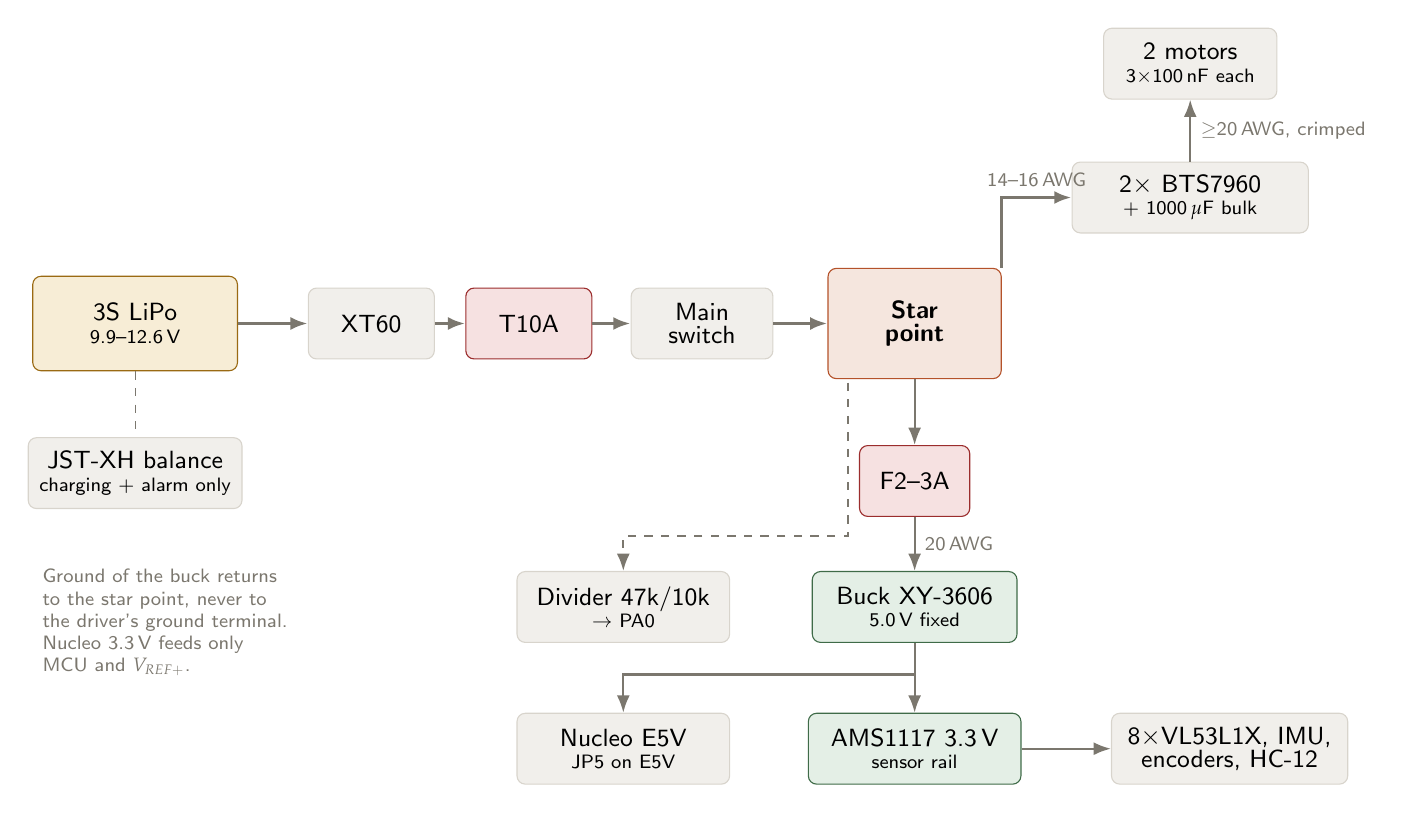
\begin{tikzpicture}[x=1cm,y=1cm]
  \node[blkW,minimum width=26mm,minimum height=12mm] (bat) at (0,0) {3S LiPo\\[-1mm]\scriptsize 9.9--12.6\,V};
  \node[blk,minimum width=16mm] (xt) at (3.0,0) {XT60};
  \node[blkB,minimum width=16mm] (f1) at (5.0,0) {T10A};
  \node[blk,minimum width=18mm] (sw) at (7.2,0) {Main\\[-1mm]switch};
  \node[blkA,minimum width=22mm,minimum height=14mm] (star) at (9.9,0) {\textbf{Star}\\[-1mm]\textbf{point}};
  \draw[arr,very thick] (bat) -- (xt);
  \draw[arr,very thick] (xt) -- (f1);
  \draw[arr,very thick] (f1) -- (sw);
  \draw[arr,very thick] (sw) -- (star);
  \node[blk,minimum width=26mm] (bal) at (0,-1.9) {JST-XH balance\\[-1mm]\scriptsize charging + alarm only};
  \draw[grey,dashed] (bat) -- (bal);
  % motor branch
  \node[blk,minimum width=30mm] (drv) at (13.4,1.6) {2$\times$ BTS7960\\[-1mm]\scriptsize + 1000\,$\mu$F bulk};
  \node[blk,minimum width=22mm] (mot) at (13.4,3.3) {2 motors\\[-1mm]\scriptsize 3$\times$100\,nF each};
  \draw[arr,very thick] (star.north east) |- (drv.west) node[lbl,pos=0.75,above] {14--16\,AWG};
  \draw[arr,thick] (drv) -- (mot) node[lbl,midway,right] {$\geq$20\,AWG, crimped};
  % logic branch
  \node[blkB,minimum width=14mm] (f2) at (9.9,-2.0) {F2--3A};
  \node[blkG,minimum width=26mm] (buck) at (9.9,-3.6) {Buck XY-3606\\[-1mm]\scriptsize 5.0\,V fixed};
  \draw[arr,thick] (star) -- (f2);
  \draw[arr,thick] (f2) -- (buck) node[lbl,midway,right] {20\,AWG};
  \node[blk,minimum width=27mm] (nuc) at (6.2,-5.4) {Nucleo E5V\\[-1mm]\scriptsize JP5 on E5V};
  \node[blkG,minimum width=27mm] (ldo) at (9.9,-5.4) {AMS1117 3.3\,V\\[-1mm]\scriptsize sensor rail};
  \node[blk,minimum width=30mm] (sens) at (13.9,-5.4) {8$\times$VL53L1X, IMU,\\[-1mm]encoders, HC-12};
  \draw[arr] (buck.south) -- ++(0,-0.4) -| (nuc.north);
  \draw[arr] (buck) -- (ldo);
  \draw[arr] (ldo) -- (sens);
  \node[blk,minimum width=27mm] (adc) at (6.2,-3.6) {Divider 47k/10k\\[-1mm]\scriptsize $\to$ PA0};
  \draw[arr,dashed] (9.05,-0.75) -- (9.05,-2.7) -| (adc.north);
  \node[lbl,align=left,anchor=north west] at (-1.3,-3.0)
     {Ground of the buck returns\\to the star point, never to\\the driver's ground terminal.\\
      Nucleo 3.3\,V feeds only\\MCU and $V_{REF+}$.};
\end{tikzpicture}
\caption{Power topology. The star point is the only place where motor and logic
currents meet; the buck converter's return goes there, not to the driver, so that
motor ripple does not travel through shared wire impedance into the sensor
supply. The balance lead is never a supply: drawing from it discharges single
cells and creates the drift that balance charging exists to prevent.}
\label{fig:power}
\end{figure}

\paragraph{Ratings.} A 35C, \qty{2.2}{Ah} pack can deliver
$35\times\qty{2.2}{A}=\qty{77}{A}$ into a short circuit; the main fuse is the
only part between a short and that current. It is slow-blow because a
simultaneous stall of both motors draws $2\times\qty{4.3}{A}=\qty{8.6}{A}$.
Dupont contacts ($\approx\qty{1}{A}$) are acceptable only for encoder and logic
lines; motor leads are crimped or soldered, because an oxidised contact adds a
drifting series resistance that the feedforward cannot see (\cref{sec:motor}).

\paragraph{Battery measurement.} $U_{PA0}=U_{bat}\cdot 10/57$: \qty{2.21}{V} at
\qty{12.6}{V}, \qty{1.74}{V} at \qty{9.9}{V}, both below the \qty{3.3}{V} ADC range;
one LSB corresponds to \qty{4.6}{mV} of pack voltage. Without the divider PA0
floats and reads \qtyrange{100}{240}{mV} of noise. \MEASURE\ actual ratio if
5\,\% resistors are used.

\paragraph{Thresholds.} Software cut-off at \qty{10.0}{V} (\qty{3.33}{V/cell}).
\VERIFY\ The buck's minimum input voltage must lie below the worst case at its
input: $\qty{9.9}{V}-\qty{0.34}{V}\ (\text{stall sag})-\qty{0.1}{V}\ (\text{wiring})
\approx\qty{9.4}{V}$; otherwise the logic browns out \emph{before} the software
cut-off acts, which presents as a random reset.

\paragraph{3.3\,V budget.} Worst case (originally eight VL53L1X ranging, HC-12
transmitting at full power; only four are fitted, so this is conservative) $\approx\qty{0.46}{A}$; the AMS1117 then dissipates
$(5-3.3)\,\text{V}\times\qty{0.46}{A}\approx\qty{0.78}{W}$ --- hot on a small
SOT-223 module. The observed overheating with the HC-12 attached (which also
pulled down the Nucleo's 3.3\,V and disturbed the ST-Link) is open item O-4.
\DECIDE\ Feed the HC-12 from \qty{5}{V} (its supply range allows it; verify that
its TXD level stays STM32-compatible), or split the sensor rail across two LDOs.

\paragraph{Commissioning order of the harness.} (1) build complete without
battery or loads; (2) continuity: XT60+ to star point, XT60$-$ to star point, no
path between them; (3) battery in, switch on, check polarity and voltage at the
star point; (4) connect the buck, measure \qty{5.00(10)}{V} \emph{unloaded};
(5) only then the Nucleo on E5V; (6) drivers and motors last. Step 4 before step
5 is the one that saves the Nucleo from a defective converter.

\paragraph{Session energy.} \MEASURE\ Mean pack current while driving. With
an assumed \qty{1}{A} mean the \qty{2.2}{Ah} pack lasts $\approx\qty{1.5}{h}$ to
\qty{70}{\percent} depth of discharge; the 15-min run is uncritical, a 3-h test
afternoon is not --- hence the second pack.
% =====================================================================
\clearpage
\section{Physical modelling}\label{sec:physics}

This section derives every model the firmware uses or will use, states its
assumptions, and identifies which parameters are measured and which are not.

\subsection{Frames and notation}\label{sec:frames}

\begin{center}
\small
\begin{tabularx}{\textwidth}{@{}lL@{}}
\toprule
\textbf{Symbol} & \textbf{Meaning}\\
\midrule
$\{W\}$, $\{B\}$ & world frame (horizontal plane, $z_W$ up; origin at X, $x_W$ along the initial heading) and body frame ($x_B$ forward, $y_B$ left, $z_B$ up, origin at the drive-axle midpoint)\\
$x,\,y,\,\theta$ & position of the axle midpoint and heading (yaw) in $\{W\}$; angles counter-clockwise positive\\
$v,\,\omega$ & forward speed and yaw rate of the body\\
$v_L,\,v_R$; $\omega_L,\,\omega_R$ & wheel ground speeds; wheel angular speeds\\
$r=D/2$, $b$ & effective rolling radius; effective wheelbase (track width), \qty{223.25}{mm} geometric\\
$i$, $\eta$ & gear ratio (motor : output), gearbox efficiency\\
$C$, $c=\pi D/C$ & encoder counts per wheel revolution; distance per count\\
$d\in[-1,1]$, $u=100\,d$ & PWM duty (signed), in \si{\percent} where so stated\\
$U_{bat}$ & battery voltage at the driver input\\
$T_s$ & sample period of the wheel loop (\qty{20}{ms})\\
$b_g$ & gyroscope bias; $s$ odometry scale state in the EKF (unitless, $\approx1$)\\
\bottomrule
\end{tabularx}
\end{center}

\subsection{Differential-drive kinematics}\label{sec:kinematics}

\begin{figure}[htbp]
\centering
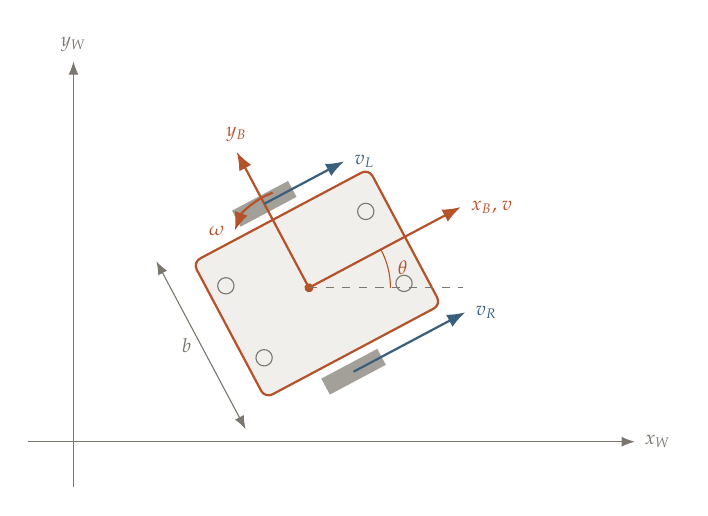
\begin{tikzpicture}[scale=1.15]
  % world axes
  \draw[-{Latex},grey] (-0.5,0) -- (6.2,0) node[right,lbl] {$x_W$};
  \draw[-{Latex},grey] (0,-0.5) -- (0,4.2) node[above,lbl] {$y_W$};
  \begin{scope}[shift={(2.6,1.7)},rotate=28]
    \draw[draw=accent,fill=greybg,thick,rounded corners=3pt] (-1.0,-0.85) rectangle (1.2,0.85);
    \fill[grey!70] (-0.35,0.95) rectangle (0.35,1.15);   % left wheel
    \fill[grey!70] (-0.35,-1.15) rectangle (0.35,-0.95); % right wheel
    \draw[grey] (0.95,0.45) circle (0.09); \draw[grey] (-0.8,0.45) circle (0.09);
    \draw[grey] (0.95,-0.45) circle (0.09); \draw[grey] (-0.8,-0.45) circle (0.09);
    \draw[-{Latex},accent,thick] (0,0) -- (1.9,0) node[right,font=\scriptsize] {$x_B$,\ $v$};
    \draw[-{Latex},accent,thick] (0,0) -- (0,1.7) node[above,font=\scriptsize] {$y_B$};
    \draw[-{Latex},cold,thick] (0,1.05) -- (1.0,1.05) node[right,font=\scriptsize,text=cold] {$v_L$};
    \draw[-{Latex},cold,thick] (0,-1.05) -- (1.4,-1.05) node[right,font=\scriptsize,text=cold] {$v_R$};
    \draw[{Latex}-{Latex},grey] (-1.35,-1.05) -- (-1.35,1.05) node[midway,left,font=\scriptsize] {$b$};
    \fill[accent] (0,0) circle (0.05);
  \end{scope}
  \draw[grey,dashed] (2.6,1.7) -- (4.3,1.7);
  \draw[accent] (3.5,1.7) arc (0:28:0.9) node[midway,right,font=\scriptsize] {$\theta$};
  \draw[-{Latex},accent,thick] (2.2,2.75) arc (110:160:0.7) node[left,font=\scriptsize] {$\omega$};
\end{tikzpicture}
\caption{Differential drive. The driven wheels sit on one axle through the body
origin; two casters carry the rest of the load. With $v_R>v_L$ the vehicle turns
left (positive $\omega$).}
\label{fig:kin}
\end{figure}

Rolling without slip gives $v_{L,R}=r\,\omega_{L,R}$. Forward and inverse
kinematics of the axle midpoint:
\begin{align}
v &= \tfrac12\,(v_R+v_L), & \omega &= \frac{v_R-v_L}{b},\label{eq:fk}\\
v_R &= v+\tfrac{b}{2}\,\omega, & v_L &= v-\tfrac{b}{2}\,\omega.\label{eq:ik}
\end{align}
The instantaneous centre of rotation (ICR) lies on the axle line at signed
distance $R=v/\omega=\tfrac b2\,(v_R+v_L)/(v_R-v_L)$; for $v_R=-v_L$ it coincides
with the axle midpoint (turn in place), which is the reason the IMU is to be
mounted there. The motion equations (unicycle model) are
\begin{equation}
\dot x = v\cos\theta,\qquad \dot y = v\sin\theta,\qquad \dot\theta=\omega,
\end{equation}
subject to the \textbf{non-holonomic constraint} (NHC) that the body cannot move
sideways:
\begin{equation}
-\dot x\sin\theta+\dot y\cos\theta = 0 .\label{eq:nhc}
\end{equation}

\paragraph{Discrete odometry.} From count increments $\Delta n_{L,R}$ in one
sample, $\Delta s_{L,R}=c_{L,R}\,\Delta n_{L,R}$,
$\Delta s=\tfrac12(\Delta s_R+\Delta s_L)$, $\Delta\theta=(\Delta s_R-\Delta s_L)/b$.
The exact update for a constant-curvature step is
\begin{equation}
\begin{aligned}
x_{k+1} &= x_k + \Delta s\,\operatorname{sinc}\!\left(\tfrac{\Delta\theta}{2}\right)\cos\!\left(\theta_k+\tfrac{\Delta\theta}{2}\right),\\
y_{k+1} &= y_k + \Delta s\,\operatorname{sinc}\!\left(\tfrac{\Delta\theta}{2}\right)\sin\!\left(\theta_k+\tfrac{\Delta\theta}{2}\right),
\qquad \theta_{k+1}=\theta_k+\Delta\theta,
\end{aligned}\label{eq:odo}
\end{equation}
with $\operatorname{sinc}(z)=\sin z/z$. Dropping the sinc factor (midpoint rule)
causes a relative chord error of $\Delta\theta^2/24$; for the fastest planned
spin ($\pm\qty{300}{mm/s}$ per wheel, $\omega=\qty{2.69}{rad/s}$, $\Delta\theta=\qty{0.054}{rad}$
at \qty{50}{Hz}) that is \num{1.2e-4} --- negligible, so the EKF uses the
midpoint rule. In the EKF, $\Delta\theta$ is taken from the gyroscope, not from
the wheels (\cref{sec:ekf}).

\paragraph{Turning envelope.} For the concept envelope of
\qtyproduct{400 x 350}{mm} with the axle at mid-length, a turn in place sweeps a
circle of diameter $2\sqrt{0.2^2+0.175^2}\,\text{m}=\qty{0.53}{m}$; \qty{0.6}{m}
of free width is planned. \VERIFY\ final chassis dimensions.

% ---------------------------------------------------------------------
\subsection{Encoder and wheel-position measurement}\label{sec:encoder}

\paragraph{Resolution.} The Hall encoder sits on the motor shaft, ahead of the
gearbox: 16 pulses per channel and revolution, decoded on both edges of both
channels ($\times4$), gives 64 counts per motor revolution and
\begin{equation}
C = 64\,i\quad\text{counts per wheel revolution}.
\end{equation}

\begin{center}
\small
\begin{tabular}{@{}lccc@{}}
\toprule
& \textbf{Motor L} & \textbf{Motor R} & \textbf{Catalogue}\\
\midrule
Counts per output revolution (hand-turned, mean of 3) & 3595 & 3618 & 3603\\
Implied gear ratio $C/64$ & 56.17 & 56.53 & 56.3\\
Rear (motor) shaft, one revolution & 64 & 64 & 64\\
\bottomrule
\end{tabular}
\end{center}

\begin{warnbox}
\textbf{Interpretation of the hand-turn counts.} Two gearboxes of the same type
have identical tooth counts and therefore identical ratios. A difference of
23\,counts/rev is \ang{2.3} of output rotation --- within reach of a felt-pen
mark plus gearbox play when turning by hand. The 0.64\,\% difference is
therefore \emph{not} accepted as a gear-ratio difference. What matters for
odometry is the \textbf{effective distance per count per wheel}, which includes
the rolling radius of each tyre and is only measurable by driving
(UMBmark, \cref{sec:umbmark}). A finer static check: wheel mounted, fixed pointer
at the tyre, 10 revolutions always approaching the mark from the same direction
(resolves $\approx\pm1$\,count/rev).
\end{warnbox}

The vehicle firmware currently uses a common $C=3584$ ($=64\times56$) together
with an effective diameter $D=\qty{72.6}{mm}$ calibrated from a straight run
(firmware 1000\,mm, tape 955\,mm at $D=\qty{76}{mm}$). Only the ratio $D/C$ is
calibrated:
\begin{equation}
c=\frac{\pi\cdot\qty{72.6}{mm}}{3584}=\qty{0.06364}{mm/count}.
\end{equation}
Switching to per-wheel counts requires raising $D$ to $72.6\cdot3606.5/3584
\approx\qty{73.06}{mm}$ to keep the mean scale.

\paragraph{Edge rate and input filter.} At the no-load output speed of
\qty{181}{rpm} the motor turns at $181\times56.17=\qty{10167}{rpm}$, giving
$10167/60\times64=\qty{10.8}{k\text{edges}/s}$, i.e.\ \qty{92}{\micro s} between
edges. The \qty{2.84}{\micro s} digital filter (\cref{sec:timers}) is 3\,\% of
that.

\paragraph{Speed quantisation.} With count differencing over one sample,
\begin{equation}
\hat v_{raw,k}=\frac{c\,\Delta n_k}{T_s},\qquad
\delta v = \frac{c}{T_s}=
\begin{cases}
\qty{3.18}{mm/s} & T_s=\qty{20}{ms}\ (50\,\text{Hz})\\
\qty{12.7}{mm/s} & T_s=\qty{5}{ms}\ (200\,\text{Hz})\\
\qty{63.6}{mm/s} & T_s=\qty{1}{ms}\ (1\,\text{kHz})
\end{cases}
\end{equation}
The firmware smooths with a first-order IIR, $\hat v_k=\hat v_{k-1}+\alpha(\hat
v_{raw,k}-\hat v_{k-1})$, $\alpha=0.5$, equivalent time constant
$\tau_f=-T_s/\ln(1-\alpha)=\qty{28.9}{ms}$ --- of the same order as the plant
time constant (\qty{50}{ms}) and therefore part of the loop's effective dead time
(\cref{sec:speedloop}). Differences are formed in \code{int16\_t}, which makes the
16-bit counter wrap-around harmless as long as $|\Delta n|<32768$ per sample.

\paragraph{Backlash.} Because the encoder sits before the gearbox, every reversal
turns the motor through the gear play before the wheel moves; those counts enter
odometry as distance that did not happen. The lost motion $\delta_b$ (counts)
is measured per wheel by calibration test \code{L} \MEASURE. Consequence for
control: \textbf{every positioning move ends from one direction}, critically
damped, without overshoot-and-return.

% ---------------------------------------------------------------------
\subsection{DC motor, gearbox and driver}\label{sec:motor}

\paragraph{Equations.} Per motor (armature resistance $R_a$, inductance $L_a$,
back-EMF constant $k_e$, torque constant $k_t$ --- numerically equal in SI
units), referred to the motor shaft:
\begin{align}
L_a\frac{\mathrm d i_a}{\mathrm dt} &= U_a - R_a i_a - k_e\,\omega_m,\label{eq:elec}\\
J_{eq}\frac{\mathrm d\omega_m}{\mathrm dt} &= k_t\,i_a - \tau_f(\omega_m) - \frac{\tau_{w}}{i\,\eta},\label{eq:mech}\\
J_{eq} &= J_m + J_{gb} + \frac{J_w + \tfrac m2\,r^2}{i^2\,\eta},\qquad \omega_m = i\,\omega_w,
\end{align}
where $\tau_w$ is the load torque at the wheel (rolling resistance, grade,
acceleration of the vehicle's share is already in $J_{eq}$) and $\tfrac m2r^2$ is
half the vehicle's translational inertia per wheel for straight driving.

\paragraph{PWM averaging.} The BTS7960 is driven sign--magnitude: one half-bridge
receives PWM (RPWM or LPWM), the other stays low, both enables high. During the
off-time both low-side switches conduct and the winding is short-circuited
(synchronous slow decay). As long as the current does not reach zero within a
PWM period (\emph{continuous conduction}, $L_a/R_a\gg\qty{50}{\micro s}$), the
winding sees the average $U_a=d\,U_{bat}$ and the duty-to-speed relation is
linear. The previous driver PWM'd the enable line, so the off-state was coast
(diode recirculation); at low duty this produces discontinuous conduction and a
non-linear low end. \MEASURE\ $L_a$ (LCR meter or current step) to confirm
continuous conduction at \qty{20}{kHz}.

\paragraph{Steady state.} With $\mathrm di/\mathrm dt=\mathrm d\omega/\mathrm dt=0$,
friction $\tau_f=\tau_C\sgn\omega_m+b_v\omega_m$ and a driver voltage drop
$U_{dr}$, eliminating $i_a$ and solving for the duty gives, for wheel speed $n$ in
rpm,
\begin{equation}
\boxed{\;d = K_v\,n + K_s\,\sgn n\;}
\quad\text{with}\quad
K_v=\frac{2\pi\,i}{60\,U_{bat}}\Bigl(k_e+\frac{R_a b_v}{k_t}\Bigr),\quad
K_s=\frac{1}{U_{bat}}\Bigl(\frac{R_a}{k_t}\Bigl(\tau_C+\frac{\tau_w}{i\eta}\Bigr)+U_{dr}\Bigr).
\label{eq:kvks}
\end{equation}
This is the model behind the feedforward, and it explains four observations:

\begin{enumerate}[leftmargin=6mm]
\item \textbf{Both constants scale with $1/U_{bat}$.} Between full (\qty{12.6}{V})
and empty (\qty{9.9}{V}) the required duty for the same speed changes by
\qty{27}{\percent}. Hence the feedforward is to be normalised,
$d_{ff}=(K_v^{V}n+K_s^{V})/U_{bat}$, with constants in volts identified together
with $U_{bat}$ (calibration \code{U} command) and $U_{bat}$ measured on PA0
\OPEN.
\item \textbf{$K_s$ contains the load.} Rolling resistance, grade and caster
friction enter through $\tau_w$; a bench (no-load) $K_s$ is a lower bound for
driving. Ground identification (\code{G}) gives the values for the vehicle.
\item \textbf{$K_s$ contains the driver.} A bipolar bridge drops volts, a MOSFET
bridge (BTS7960: tens of m$\Omega$ against an armature of $\approx\qty{2.8}{\ohm}$)
practically nothing. The BTS7960 dead zone (\qty{7.0}{\percent} mean, wheels in air)
is indeed lower than the bench intercepts (11.0/12.7\,\%).
\item \textbf{$K_v$ is a motor property.} It should not change with the driver.
Bench: $1/K_v$ corresponds to \qty{7.73}{(mm/s)/\percent} (L) and \qty{7.50}{(mm/s)/\percent}
(R); BTS7960 identification: \qty{7.60}{(mm/s)/\percent} mean. Agreement to
\qty{2}{\percent} --- a consistency check that the identification is sound
(differences in $U_{bat}$ between the two sessions are not recorded \VERIFY).
\end{enumerate}

\paragraph{Dynamics.} Neglecting $L_a$ (electrical time constant $\ll$ mechanical),
\cref{eq:elec,eq:mech} reduce to a first-order plant from duty to speed,
\begin{equation}
G(s)=\frac{V(s)}{U(s)}=\frac{K}{\tau_m s+1},\qquad
\tau_m=\frac{J_{eq}R_a}{k_e k_t+R_a b_v},\label{eq:plant}
\end{equation}
identified on the BTS7960 with wheels in the air as $K=\qty{7.596}{(mm/s)/\percent}$,
$\tau_m=\qty{50}{ms}$, no measurable dead time. On the ground $J_{eq}$ grows by
$\tfrac m2r^2/(i^2\eta)$; with an assumed $m=\qty{3}{kg}$ that is
$\approx\qty{6e-7}{kg.m^2}/\eta$ at the motor shaft --- comparable to the rotor
inertia of a \qty{37}{mm} motor, so $\tau_m$ on the ground may be noticeably
larger \MEASURE\ (test \code{G}, step response on the floor).

\paragraph{Parameter estimate (not measured).} Assuming the bench supply was
\qty{12}{V}: at $d=1$ the model gives \qty{181}{rpm}, of which the fraction
$K_s=0.11$ of the voltage covers friction, so
$k_e\approx(1-K_s)U/\omega_m=0.89\cdot12/\qty{1065}{rad/s}\approx\qty{10.0}{mV.s/rad}$.
With the catalogue stall current, $R_a\approx\qty{12}{V}/\qty{4.3}{A}=\qty{2.8}{\ohm}$
and the stall torque at the motor shaft
$\approx k_t\cdot\qty{4.3}{A}=\qty{43}{mN.m}$, i.e.\ $\approx\qty{2.4}{N.m}\cdot\eta$ at the
output. Even with a poor $\eta$ this is several times the catalogue
\qty{3.4}{kgf.cm} (\qty{0.33}{N.m}), which therefore is almost certainly the
\emph{rated} and not the stall torque. \VERIFY\ bench voltage, and \ASK\ vendor.

% ---------------------------------------------------------------------
\subsection{Friction}\label{sec:friction}

The drivetrain friction is modelled as Coulomb + viscous + Stribeck:
\begin{equation}
\tau_f(\omega)=\Bigl(\tau_C+(\tau_S-\tau_C)\,e^{-(\omega/\omega_S)^2}\Bigr)\sgn\omega + b_v\,\omega .
\end{equation}
Static friction $\tau_S$ exceeds kinetic friction $\tau_C$. On the bench this is
directly visible:

\begin{center}
\small
\begin{tabular}{@{}lcccc@{}}
\toprule
& \textbf{Breakaway from rest} & \textbf{Running intercept $K_s$} & \textbf{Difference} & \textbf{Ratio}\\
\midrule
Motor L & 0.141 & 0.110 & 0.031 & 1.28\\
Motor R & 0.169 & 0.127 & 0.042 & 1.33\\
\bottomrule
\end{tabular}
\end{center}

\textbf{Consequences.} (i) The \emph{running} intercept belongs in the speed
feedforward; the breakaway value would overcompensate every normal movement.
(ii) Starting from rest needs more --- either the integrator winds up through the
gap (slow, produces stick-slip with a brief slip of the wheel) or the
feedforward switches to the breakaway value below a speed threshold (variant B,
\cref{sec:speedloop}). (iii) The breakaway scatters by $\approx\pm5\,\%$ with
shaft angle (gear meshing), so it is measured as a distribution, not a value
(test \code{B}: six trials per direction, maximum used).

% ---------------------------------------------------------------------
\subsection{Longitudinal vehicle dynamics and motor margin}\label{sec:longdyn}

On a grade $\alpha$ with rolling-resistance coefficient $c_{rr}$, the traction
force both wheels must deliver is
\begin{equation}
F = m\bigl(g(\sin\alpha+c_{rr}\cos\alpha)+a\bigr),\qquad
\tau_{w}=\tfrac12 F r\ \text{per wheel}.
\end{equation}
Evaluated with assumed $m=\qty{3}{kg}$ \MEASURE, $c_{rr}=0.02$ (hard tyre on
paving, assumption), $r=\qty{36.3}{mm}$:

\begin{center}
\small
\begin{tabular}{@{}lccccc@{}}
\toprule
\textbf{Grade} & \textbf{Accel.} & \textbf{$F$ [N]} & \textbf{$\tau_w$ per wheel [N\,m]} & \textbf{[kgf\,cm]} & \textbf{share of 3.4\,kgf\,cm}\\
\midrule
\ang{0} & 0 & 0.59 & 0.011 & 0.11 & 3\,\%\\
\ang{0} & \qty{0.3}{m/s^2} & 1.49 & 0.027 & 0.28 & 8\,\%\\
\ang{5} & 0 & 3.15 & 0.057 & 0.58 & 17\,\%\\
\ang{8} & \qty{0.3}{m/s^2} & 5.58 & 0.101 & 1.03 & 30\,\%\\
\bottomrule
\end{tabular}
\end{center}

Torque is not the constraint even if \qty{3.4}{kgf.cm} were the stall rating.
The binding limits are elsewhere:

\begin{itemize}[leftmargin=6mm]
\item \textbf{Wheel diameter versus edges.} The lip at the ramp must be crossed
by wheels and casters. (The step marked on the northern path in
\cref{fig:course} runs \emph{parallel} to the direction of travel: it is a
drop-off to stay clear of and a lateral reference, not an edge to climb
\VERIFY\ on site.) A free
(caster) wheel of radius $r_c$ carrying normal load $N$ and pushed horizontally
against an edge of height $h<r_c$ starts to climb only when the push exceeds
\begin{equation}
F_{push}=N\tan\beta=N\,\frac{\sqrt{h\,(2r_c-h)}}{r_c-h},\qquad \cos\beta=\frac{r_c-h}{r_c}.
\end{equation}
Example: $r_c=\qty{25}{mm}$, $h=\qty{10}{mm}$ gives $F_{push}=1.33\,N$ --- the
casters can need more force than the whole vehicle needs on an \ang{8} ramp. For a
driven wheel the same geometry applies with the friction limit $\mu N$ in place of
the push. \MEASURE\ ramp-lip height --- this gates wheel and caster size.
\item \textbf{Traction.} The drive force is limited by $\mu N_d$, where $N_d$ is
the normal force on the drive wheels. With the axle at mid-length and casters
fore and aft, $N_d<mg$; at a crest or in a dip the casters can unload the drive
wheels. \VERIFY\ load split on the finished chassis.
\item \textbf{Speed.} Bench no-load maxima \qty{688}{mm/s} (L) and \qty{673}{mm/s}
(R) at $d=1$; BTS7960, wheels in air: highest measured \qty{680}{mm/s}. A
commanded \qty{800}{mm/s} (\code{D2000} test, 8 Oct) saturated and fell short
(1766/1759\,mm). Recommended ceiling: \qty{75}{\percent} of the weaker wheel at
\qty{10.5}{V}: $654.5\times10.5/12\times0.75\approx\qty{430}{mm/s}$ ---
\code{V\_NOM\_MAX} should drop from 800 to 450--500 (open item O-5).
\item \textbf{Minimum speed.} The weaker wheel's breakaway limits slow creeping;
estimated $\approx\qty{30}{mm/s}$ \VERIFY\ with test \code{B} on the BTS7960.
\end{itemize}

\subsection{Rotation, casters and effective wheelbase}\label{sec:rotation}

Yaw dynamics, with $I_z$ the yaw inertia and $M_c$ the caster and tyre-scrub
moments,
\begin{equation}
I_z\,\dot\omega = \tfrac b2\,(F_R-F_L) - M_c .
\end{equation}
Swivel casters produce a transient moment whenever the direction of travel
changes (they must flip), which disturbs the first centimetres after a turn or
reversal. Procedure consequence: after a turn in place drive
\qtyrange{20}{30}{cm} straight before re-acquiring references. The tyre contact
patches have finite width, so the \emph{effective} wheelbase differs from the
geometric \qty{223.25}{mm}; it is identified by UMBmark (factor $E_b$) and by
10-turn spins (\code{W$\pm$3600}).

% ---------------------------------------------------------------------
\subsection{Odometry error model}\label{sec:odoerr}

\paragraph{Systematic errors} (repeatable, calibratable):
\begin{itemize}[leftmargin=6mm]
\item \textbf{Scale error} $\varepsilon_s$ (mean $D/C$ wrong): along-track error
$\delta s=\varepsilon_s\,s$.
\item \textbf{Unequal wheels} $E_d=D_R/D_L\neq1$, or $\varepsilon=1-E_d$: driving
equal counts makes the vehicle turn with curvature $\kappa=\varepsilon/b$, so
the lateral deviation grows \textbf{quadratically},
\begin{equation}
y(s)=\frac{\varepsilon\,s^2}{2b}.\label{eq:drift}
\end{equation}
\item \textbf{Wheelbase error} $E_b$: wrong encoder-derived heading change in
turns, proportional to the angle turned.
\item \textbf{Backlash} $\delta_b$: lost motion per reversal.
\end{itemize}

With the hand-turn values ($\varepsilon=0.64\,\%$, $b=\qty{0.223}{m}$) and a
common count constant, \cref{eq:drift} predicts a drift to the right of
\qty{14}{mm} after \qty{1}{m}, \qty{57}{mm} after \qty{2}{m} and \qty{36}{cm}
after \qty{5}{m} (curvature \qty{0.0287}{m^{-1}}, \ang{1.6} per metre) --- the
direction actually observed on the vehicle.

\begin{coldbox}
\textbf{Telling causes apart by the shape of the drift.} Drive \code{D1000},
\code{D2000}, \code{D4000} and measure the lateral offset $y$:
$y\propto s^2$ $\Rightarrow$ scale difference between the wheels ($E_d$,
fixed by UMBmark); $y\propto s$ $\Rightarrow$ constant heading error from the
start (placement, backlash, start transient); $y\approx$ const.\ after the first
metre $\Rightarrow$ L/R tracking difference during the ramp-up (fixed by the
synchronisation term, \cref{sec:sync}).
\end{coldbox}

\paragraph{Non-systematic errors} (random): wheel slip on dust, gravel or wet
paving, uneven ground, the step, caster disturbances. They cannot be calibrated,
only detected: the \textbf{slip detector} compares the encoder yaw rate
$(\Delta s_R-\Delta s_L)/(b\,T_s)$ with the bias-corrected gyro rate; a
persistent difference inflates the process noise of the distance increment in the
EKF (\cref{sec:ekf}). With the gyro providing heading, $E_d$ and $E_b$ no longer
corrupt the EKF's heading --- but they still corrupt the encoder-only firmware in
use today, the slip detector and the L/R synchronisation, which is why UMBmark
remains worth doing.

\subsection{Inertial model and slope projection}\label{sec:imumodel}

The gyroscope measures the body-frame rate with bias, noise and a temperature
dependent offset,
\begin{equation}
\omega_{z,meas}=\omega_z+b_g(T,t)+n_\omega,\qquad
\dot b_g = n_b\ (\text{random walk}).
\end{equation}
Heading integrated from a residual bias $\delta b$ produces, at speed $v$ over
distance $s$, a lateral error $y=\delta b\,s^2/(2v)$; angle random walk
$N$ [$^\circ/\sqrt{\mathrm{h}}$] adds $\sigma_\theta(t)=N\sqrt t$. Both are
determined from an Allan-variance run of the selected IMU \MEASURE.

During every stop the true rate is zero, so the mean of the gyro output over the
stop window is a direct bias measurement (ZUPT). For white rate noise of standard
deviation $\sigma_\omega$ at rate $f$, a window $T_Z$ gives
$\sigma_{b}=\sigma_\omega/\sqrt{f\,T_Z}$; the \qty{10}{s} waypoint stops are such
windows by rule.

\paragraph{Slope.} The gyro measures rotation about the \emph{body} $z$ axis; the
heading needs rotation about the world vertical. With roll $\phi$ and pitch
$\vartheta$ (ZYX Euler angles) and body rates $p,q,r$,
\begin{equation}
\dot\psi=\frac{q\sin\phi+r\cos\phi}{\cos\vartheta}.\label{eq:euler}
\end{equation}
Turning \ang{90} on a ramp of \ang{6} pitch while integrating $r$ alone turns
in reality \ang{90.50}; at \ang{8} \ang{90.88}. Over a following \qty{40}{m}
segment that is \qty{35}{cm} and \qty{62}{cm} of cross-track error --- larger
than the rest of the budget. Mitigations: (1) \textbf{turn only on level ground}
(removes almost all of it); (2) project with \cref{eq:euler}, roll and pitch from
a complementary filter on accelerometer and gyro (valid because specific force
is dominated by gravity at these accelerations). Path cross-fall of
\qtyrange{1}{2}{\percent} is irrelevant.

% ---------------------------------------------------------------------
\subsection{Range-sensor models (VL53L1X)}\label{sec:tofmodel}

The VL53L1X is a \qty{940}{nm} single-photon time-of-flight sensor with a
\ang{27} full field of view, a programmable region of interest (ROI, minimum
$4\times4$ SPADs), distance modes short ($\approx\qty{1.3}{m}$) to long
($\approx\qty{4}{m}$ indoors, much less in sunlight) and per-measurement outputs
of range, \emph{signal rate}, \emph{ambient rate} and \emph{sigma} (estimated
range standard deviation). The measurement belongs to the middle of the
integration window (timing budget), which matters for timestamping.

\paragraph{Downward versus angled mounting.} Mounted at height $h$ and looking
straight down, the sensor reads $r=h/(\cos\phi\cos\vartheta)$; pitch enters
only to second order: at \ang{5} the error is \qty{0.38}{\percent},
\qty{0.76}{mm} at $h=\qty{200}{mm}$. Mounted at angle $\alpha$ to the ground it
reads $r=h/\sin\alpha$ with first-order sensitivity
\begin{equation}
\frac{\partial r}{\partial\alpha}=-\frac{h\cos\alpha}{\sin^2\alpha}
\;\Rightarrow\; \qty{1.21}{cm/\degree}\ \text{at}\ h=\qty{20}{cm},\ \alpha=\ang{30},
\end{equation}
so a \ang{4} pitch on the ramp would move the reading by \qty{4.8}{cm} --- more
than the \qtyrange{3}{4}{cm} rubber edging it is meant to detect. Hence all
ground sensors look straight down.

\paragraph{Footprint.} The illuminated spot has diameter $2h\tan(\mathrm{FoV}/2)$:
\begin{center}
\small
\begin{tabular}{@{}lcc@{}}
\toprule
& $h=\qty{200}{mm}$ & $h=\qty{300}{mm}$\\
\midrule
Full FoV \ang{27} & \qty{96}{mm} & \qty{144}{mm}\\
ROI $4\times4$, FoV $\approx\ang{15}$ & \qty{53}{mm} & \qty{79}{mm}\\
\bottomrule
\end{tabular}
\end{center}
A short baffle tube further limits stray light. The mounting height therefore
directly sets the lateral resolution of the edge measurement; low mounting is
better (\qtyrange{100}{200}{mm}) \DECIDE.

\paragraph{Surface classification.} Grass is a diffuse, unevenly high scatterer:
high sigma, low signal rate. Paving: low sigma, high signal rate. Rubber edging:
low sigma at a different height. This two-feature, three-class discriminator is
independent of colour and illumination and also works where there is no height
step. \MEASURE\ thresholds outdoors, noon and afternoon.

\paragraph{Lateral heading fit.} A sideways-looking sensor passing a straight
face (bench, kerb, wall) measures $r_i=d_0-s_i\sin\Delta\psi+n_i$, with
$\Delta\psi$ the heading relative to the face and $s_i$ the distance travelled.
A least-squares line fit over a baseline $S$ with $N$ evenly spaced samples has
slope variance $\sigma_r^2/\sum(s_i-\bar s)^2\approx12\,\sigma_r^2/(NS^2)$, so
\begin{equation}
\sigma_{\Delta\psi}\approx\frac{\sigma_r\sqrt{12}}{S\sqrt N}.\label{eq:headingfit}
\end{equation}
With pessimistic $\sigma_r=\qty{2}{cm}$, $S=\qty{2}{m}$, $N=250$ (\qty{50}{Hz},
\qty{0.4}{m/s}): $\sigma_{\Delta\psi}=\ang{0.13}$, i.e.\ \qty{8.8}{cm} lateral
over a following \qty{40}{m} --- against \qty{21}{cm} for a \ang{0.3} entry
error without the fit. The absolute heading of the face must be known from the
course survey to $\approx\ang{0.5}$ or better, or the fit only gives a relative
heading.

\paragraph{Cylindrical landmarks.} A post seen sideways produces a notch in the
range profile; its centre (midpoint of the flanks) gives the along-track
position. A wider spot widens the notch symmetrically but does not shift it, so
the flank-midpoint method remains valid with the VL53L1X.
% =====================================================================
\clearpage
\section{Measured parameters and identification}\label{sec:measured}

\subsection{Bench session, week 5 (previous driver, no load)}\label{sec:bench}

Set-up: L298-style opto-isolated driver on a laboratory supply, one motor at a
time, no wheel, bench firmware (\code{BENCH\_README.md}) with a 1\,kHz tick and
raw-duty sweeps. Two sweeps per motor, nine duty steps from 20\,\% to 100\,\%,
linear least-squares fit of duty on speed; breakaway from 3--4 slow ramps.

\begin{center}
\small
\begin{tabular}{@{}lccl@{}}
\toprule
\textbf{Quantity} & \textbf{Motor L} & \textbf{Motor R} & \textbf{Note}\\
\midrule
$K_v$ [duty/rpm] & 0.00492 & 0.00507 & slope of the running fit\\
$K_s$ [duty] & 0.110 & 0.127 & intercept = kinetic friction\\
Breakaway duty & 0.141 & 0.169 & static friction, $\pm5\,\%$ scatter\\
No-load speed at $d=1$ & \qty{181}{rpm} & \qty{177}{rpm} & catalogue 178\\
Linearity & $R^2>0.999$ & $R^2>0.999$ & model \cref{eq:kvks} confirmed\\
Counts per output rev. & 3595 & 3618 & hand-turned, 3 rev.\\
Encoder A--B resistance & \qty{\approx6}{k\ohm} & \qty{\approx6}{k\ohm} & symmetric $\Rightarrow$ $2\times\qty{3}{k\ohm}$ pull-ups via V+\\
Encoder sign (bench wiring) & $-1$ & $+1$ & harness-dependent (vehicle: $+1/-1$)\\
\bottomrule
\end{tabular}
\end{center}

\textbf{Encoder V+ identification without power.} Because the open-collector
pull-ups hang on V+, the wire showing $\approx\qty{3}{k\ohm}$ to \emph{both} A and
B is V+, an open wire to both is GND, and a pair reading a few ohms is the
winding. Recording the \qty{6}{k\ohm} per motor at goods-in gives a later
reference for a detached pull-up or a damaged output.

\textbf{Previous driver truth table} (6\,V, 100\,mA limit, motors
disconnected): the state IN1\,=\,IN2\,=\,1 drew no current, ruling out
shoot-through; brake versus coast was not resolved. With the move to the
BTS7960 this is closed: each BTS7960 is a half-bridge with internal dead time;
RPWM\,=\,LPWM\,=\,1 drives both outputs high (a brake to the supply rail), which
is not destructive, but the firmware still never produces it.

\subsection{Identification on the BTS7960 (9 Oct, wheels in the air)}\label{sec:ident}

Step and ramp experiments on both wheels, first-order-plus-dead-time fit:

\begin{center}
\small
\begin{tabular}{@{}lll@{}}
\toprule
\textbf{Quantity} & \textbf{Value} & \textbf{Note}\\
\midrule
Static gain $K$ & \qty{7.596}{(mm/s)/\percent} & both wheels, slope of $v_{ss}(u)$\\
Time constant $\tau_m$ & \qty{50}{ms} & \\
Plant dead time $L$ & \qty{0}{ms} & design delay $\theta=L+T_s+\text{filter}=\qty{49}{ms}$\\
Dead zone $u_0$ & \qty{7.0}{\percent} & mean of both wheels\\
Feedforward L & $9.8\,\% + 0.1275\,\%/(\text{mm/s})$ & per-wheel fit\\
Feedforward R & $4.1\,\% + 0.1361\,\%/(\text{mm/s})$ & per-wheel fit\\
Highest speed & \qty{680}{mm/s} at 100\,\% & \\
\bottomrule
\end{tabular}
\end{center}

\begin{warnbox}
\textbf{Plausibility of the per-wheel intercepts.} On the bench the right motor
had the \emph{higher} intercept (0.127 vs 0.110); on the BTS7960 it has the
\emph{lower} one (4.1\,\% vs 9.8\,\%), while the slope ordering (R weaker) is
preserved. Slope and intercept of a line fit are negatively correlated, and a
fit over a narrow speed range trades one against the other. \VERIFY\ with the
calibration sweep \code{K} (16 levels, 2 repetitions, standard errors reported)
and the closed-loop ground sweep \code{G}; record $U_{bat}$ for both.
\end{warnbox}

\begin{figure}[htbp]
\centering
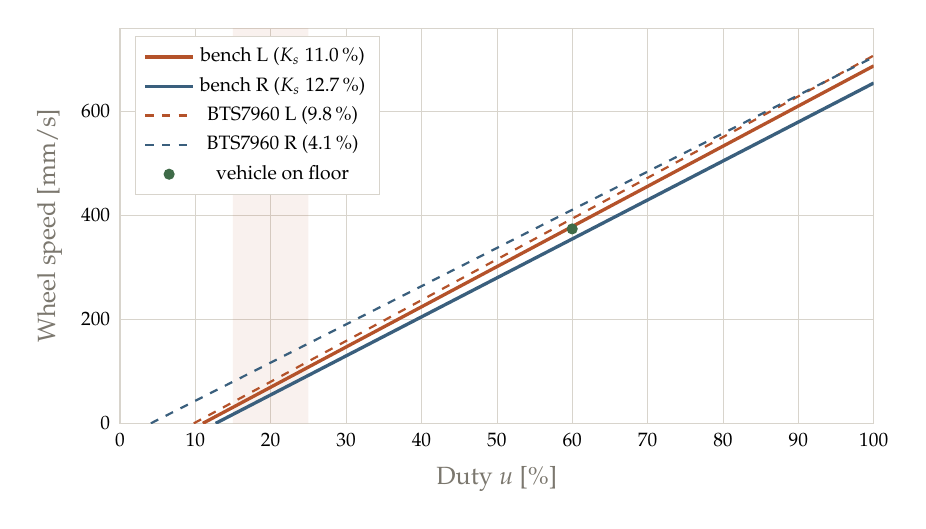
\begin{tikzpicture}
\begin{axis}[mr,
  width=0.92\textwidth, height=66mm,
  xlabel={Duty $u$ [\%]}, ylabel={Wheel speed [mm/s]},
  xmin=0, xmax=100, ymin=0, ymax=760,
  legend style={at={(0.02,0.98)},anchor=north west},
]
  \addplot[draw=none,fill=accent,opacity=0.08,forget plot]
    coordinates {(15,0)(25,0)(25,760)(15,760)} \closedcycle;
  \addplot[accent,very thick,domain=11.0:100,samples=2]{(x-11.0)*7.726};
  \addplot[cold,very thick,domain=12.7:100,samples=2]{(x-12.7)*7.498};
  \addplot[accent,thick,dashed,domain=9.8:100,samples=2]{(x-9.8)/0.1275};
  \addplot[cold,thick,dashed,domain=4.1:100,samples=2]{(x-4.1)/0.1361};
  \addplot[only marks,mark=*,mark size=1.8pt,good] coordinates {(60,374)};
  \legend{bench L ($K_s$ 11.0\,\%), bench R ($K_s$ 12.7\,\%),
          BTS7960 L (9.8\,\%), BTS7960 R (4.1\,\%), vehicle on floor, 60\,\%}
  \node[font=\scriptsize\color{accent}] at (axis cs:20,700) {APPROACH};
\end{axis}
\end{tikzpicture}
\caption{Duty-to-speed characteristics. Solid: bench (old driver, lab supply,
no load), converted with $D=\qty{72.6}{mm}$. Dashed: BTS7960 identification,
wheels in the air. Dot: open-loop measurement on the floor at 60\,\% (8 Oct),
\qty{374}{mm/s} against \qty{379}{mm/s} predicted by the bench model for the left
wheel --- the load on level paving costs about \qty{1}{\percent}. The shaded band
is the duty range of slow final approaches, where friction modelling matters most.}
\label{fig:kvplot}
\end{figure}

\subsection{Vehicle tests (8 Oct)}

\begin{center}
\small
\begin{tabularx}{\textwidth}{@{}lccL@{}}
\toprule
\textbf{Test} & \textbf{L [mm]} & \textbf{R [mm]} & \textbf{Finding}\\
\midrule
\code{D1000}, TIM6 at 1\,kHz (wrong) & 292.3 & 288.5 & tick 20$\times$ too fast $\Rightarrow$ profile too short\\
\code{D1000}, PLLM /8, TIM6 41.7\,Hz & 994.5 & 994.1 & settle timeout 5.5\,mm before the target\\
\code{D1000} after clock fix, $D=\qty{76}{mm}$ & 999.5 & 1000.3 & firmware view; tape: \qty{955}{mm}\\
$\Rightarrow$ effective diameter & \multicolumn{2}{c}{$76\times955/1000=\qty{72.59}{mm}$} & entered as 72.6\,mm (with $C=3584$)\\
\code{D2000}, \code{V800}, short ramps & 1766.3 & 1758.9 & saturation: \qty{800}{mm/s} above the drive limit\\
Open loop 60\,\%, floor & 374\,mm/s & --- & bench model predicts 379\,mm/s\\
\bottomrule
\end{tabularx}
\end{center}

All firmware distances are encoder distances; only the 955\,mm tape value is
ground truth. Repeatability of the end position and lateral drift on long runs
have not been measured \MEASURE.

\subsection{Motor pairing}\label{sec:pairing}

\begin{center}
\small
\begin{tabular}{@{}lccc@{}}
\toprule
\textbf{Quantity (bench, equal duty)} & \textbf{L} & \textbf{R} & \textbf{Difference}\\
\midrule
Speed at 30\,\% duty & \qty{39.3}{rpm} & \qty{35.1}{rpm} & +12\,\% left\\
$K_v$ & 0.00492 & 0.00507 & 3\,\%\\
Breakaway duty & 0.141 & 0.169 & +20\,\% right\\
No-load speed & \qty{181}{rpm} & \qty{177}{rpm} & 2\,\%\\
Implied gear ratio & 56.17 & 56.53 & 0.64\,\% (see \cref{sec:encoder})\\
\bottomrule
\end{tabular}
\end{center}

The speed difference at low duty is dominated by friction (breakaway +20\,\%,
slope only 3\,\%): at 30\,\% the left motor has more net voltage above its
friction threshold. Consequences: open loop with a common duty the vehicle
drives an arc; the per-wheel feedforward removes most of it before any loop
closes; the per-wheel speed loop removes the rest; matching motors by purchase
would be expensive and would drift with wear. \VERIFY\ Re-measure with wheels,
vehicle mass and battery; load friction may not scale equally on both sides.

\subsection{Calibration status}\label{sec:calibstatus}

\begin{center}
\small
\begin{tabularx}{\textwidth}{@{}lcL@{}}
\toprule
\textbf{Constant} & \textbf{Status} & \textbf{Source / next step}\\
\midrule
Encoder signs, motor signs & \tg{done} & vehicle: \code{ENC\_L/R = +1/-1}, \code{MOT\_L/R = -1/+1}; re-check with \code{C} after any harness change\\
$K_v$, $K_s$ (no load) & \tg{done} & bench + BTS7960 wheels-in-air\\
$K_v$, $K_s$ under load & \tw{open} & calibration \code{G} on the floor\\
Breakaway on BTS7960 & \tw{open} & \code{B}; code still uses bench 14.1/16.9\,\%\\
$\tau_m$ under load & \tw{open} & \code{G}/\code{K} level changes\\
Mean scale $D/C$ & \tg{done} & 72.6\,mm / 3584; repeat \code{D5000}$\times3$ per surface\\
Per-wheel mm/count ($E_d$) & \tw{open} & UMBmark \code{Q$\pm$2000}$\times5$\\
Effective wheelbase ($E_b$) & \tw{open} & UMBmark, \code{W$\pm$3600}\\
Backlash $\delta_b$ & \tw{open} & \code{L}\\
Driver duty floor $U_{min}$ & \tw{open} & oscilloscope on the BTS7960 output\\
Battery divider ratio & \tw{open} & multimeter vs ADC\\
Gyro bias, ARW, temperature & \tk{after IMU} & Allan variance, temperature run\\
VL53L1X thresholds, $\sigma_r$ & \tk{after fitting} & outdoor afternoon test\\
\bottomrule
\end{tabularx}
\end{center}
% =====================================================================
\clearpage
\section{Control system}\label{sec:control}

\subsection{Structure of the wheel cascade (implemented)}\label{sec:cascade}

Each wheel has its own cascade, executed in the TIM6 interrupt at \qty{50}{Hz}
(\code{Control\_Tick()}): a time-based trapezoidal profile generates
$v_{prof}(t)$ and $x_{prof}(t)$; a P position loop corrects deviations from
$x_{prof}$; an inner speed loop with model feedforward and PI feedback produces the
duty. The two cascades are coupled by a synchronisation term that keeps the
wheel position errors equal, i.e.\ suppresses heading transients.

\begin{figure}[htbp]
\centering
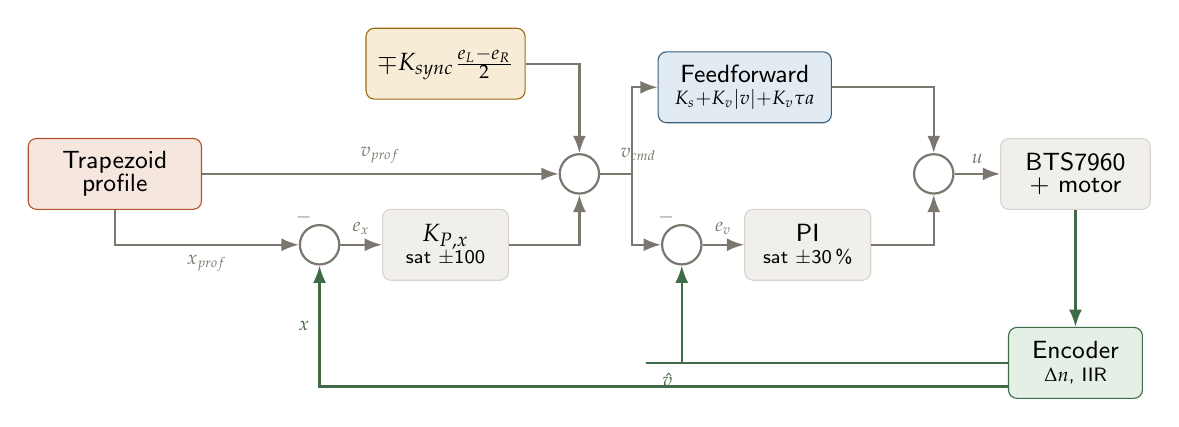
\begin{tikzpicture}[x=1cm,y=1cm]
  \node[blkA,minimum width=22mm] (prof) at (0,0) {Trapezoid\\[-1mm]profile};
  \node[sum] (s1) at (2.6,-0.9) {};
  \node[blk,minimum width=16mm] (kp) at (4.2,-0.9) {$K_{P,x}$\\[-1mm]\scriptsize sat $\pm$100};
  \node[sum] (s2) at (5.9,0) {};
  \node[blkK,minimum width=22mm] (ff) at (8.0,1.1) {Feedforward\\[-1mm]\scriptsize$K_s{+}K_v|v|{+}K_v\tau a$};
  \node[sum] (s3) at (7.2,-0.9) {};
  \node[blk,minimum width=16mm] (pi) at (8.8,-0.9) {PI\\[-1mm]\scriptsize sat $\pm$30\,\%};
  \node[sum] (s4) at (10.4,0) {};
  \node[blk,minimum width=19mm] (pl) at (12.2,0) {BTS7960\\[-1mm]+ motor};
  \node[blkG,minimum width=17mm] (enc) at (12.2,-2.4) {Encoder\\[-1mm]\scriptsize$\Delta n$, IIR};
  \node[blkW,minimum width=17mm] (sync) at (4.2,1.4) {$\mp K_{sync}\tfrac{e_L-e_R}{2}$};
  \draw[arr] (prof.east) -- node[lbl,above] {$v_{prof}$} (s2.west);
  \draw[arr] (prof.south) |- node[lbl,pos=0.75,below] {$x_{prof}$} (s1.west);
  \draw[arr] (s1) -- node[lbl,above] {$e_x$} (kp);
  \draw[arr] (kp.east) -| (s2.south);
  \draw[arr] (sync.east) -| (s2.north);
  \draw[arr] (s2.east) -- ++(0.4,0) |- (ff.west);
  \draw[arr] (s2.east) -- ++(0.4,0) |- (s3.west);
  \node[lbl] at (6.65,0.25) {$v_{cmd}$};
  \draw[arr] (s3) -- node[lbl,above] {$e_v$} (pi);
  \draw[arr] (pi.east) -| (s4.south);
  \draw[arr] (ff.east) -| (s4.north);
  \draw[arr] (s4) -- node[lbl,above] {$u$} (pl);
  \draw[arrG] (pl) -- (enc);
  \draw[arrG] (enc.west) -- ++(-4.6,0) -| node[lbl,pos=0.3,below,text=good] {$\hat v$} (s3.south);
  \draw[arrG] (enc.west) ++(0,-0.3) -- (2.6,-2.7) -- node[lbl,pos=0.5,left,text=good] {$x$} (s1.south);
  \node[lbl] at (2.4,-0.55) {$-$}; \node[lbl] at (7.0,-0.55) {$-$};
\end{tikzpicture}
\caption{Wheel cascade per side (L and R identical, own constants). The
feedforward carries the bulk of the duty; the PI only corrects model error; the
position loop only corrects the integral of what the speed loop missed.}
\label{fig:cascade}
\end{figure}

\subsection{Actuation layer}\label{sec:actuation}

\begin{itemize}[leftmargin=6mm]
\item \textbf{Mapping.} $d\cdot\sigma_{mot}>0$ ($\sigma_{mot}=$ \code{MOT\_x\_SIGN}) $\Rightarrow$ RPWM carries
the PWM and LPWM is 0; otherwise the reverse. Both enables of a module are bridged
on one GPIO (EN\_L = PB12, EN\_R = PB13). A single setter function is the only
writer of CCR1--4 and the EN lines; it sets the inactive channel to 0
\emph{before} the active one, so no instruction-length state with both inputs
high exists.
\item \textbf{Frequency.} \qty{20}{kHz} --- inaudible and within the BTS7960's
\qty{25}{kHz} limit. The 5-vs-10\,kHz decision of the concept (old driver with a
\qty{10}{kHz} limit and a large duty floor) is superseded. \MEASURE\ the real
output floor $U_{min}$ at \qty{20}{kHz} with an oscilloscope; if it approaches the
\qty{7}{\percent} dead zone, \qty{10}{kHz} halves it at the cost of audible noise.
\item \textbf{Reversal.} The bench firmware enforces \qty{50}{ms} coast on every
reversal and a slew limit of 0$\to$100\,\% in \qty{500}{ms}; the vehicle firmware
avoids end-of-move reversals altogether (backlash, \cref{sec:encoder}).
\item \textbf{Defined off-state.} EN lines have internal and external
(\qty{10}{k\ohm}) pull-downs; TIM1 idle state is ``reset'' (outputs low while MOE
is cleared). \code{Error\_Handler} must actively clear CCR1--4 and pull EN low
(open item O-12) --- otherwise a fault leaves PWM running with enables high.
\end{itemize}

\subsection{Wheel speed control}\label{sec:speedloop}

\paragraph{Control law.} For each wheel, with $v_{cmd}$ the commanded speed,
$\hat v$ the filtered measured speed and $e_v=v_{cmd}-\hat v$:
\begin{equation}
\begin{aligned}
u &= \underbrace{\sgn(v_{cmd})\bigl(K_s^{*}+K_v|v_{cmd}|\bigr)+K_v\,\tau_m\,a_{prof}}_{\text{feedforward}}
   +\underbrace{K_p\,e_v+I_k}_{\text{PI}},\\
I_k &= \sat_{\pm30\,\%}\bigl(I_{k-1}+K_i\,e_v\,T_s\bigr).
\end{aligned}
\label{eq:speedlaw}
\end{equation}
\begin{itemize}[leftmargin=6mm]
\item $K_s^{*}=K_{s,break}$ while the wheel stands ($|\hat v|<\qty{3}{mm/s}$),
$K_s$ (running intercept) once it rolls ($|\hat v|>\qty{8}{mm/s}$), with
hysteresis in between. This is the friction model of \cref{sec:friction} made
explicit; it replaced the earlier ``kick'' (40\,\% for up to 5 ticks), which acted
per wheel independently and let one wheel break away before the other --- a
heading error at every start.
\item $K_v\tau_m a$ is the inertia feedforward: for the first-order plant
\cref{eq:plant}, the duty that produces $\dot v=a$ on top of steady state is
$\tau_m a/K$, and $1/K=K_v$.
\item Unit conversion of the bench constants:
$K_v^{[\%/(mm/s)]}=K_v^{[duty/rpm]}\cdot100\cdot60/(\pi D)$, i.e.\
0.1294 (L) and 0.1334 (R) \si{\percent/(mm/s)}.
\end{itemize}

\paragraph{Tuning by SIMC.} For a first-order plant with dead time,
$G(s)=Ke^{-\theta s}/(\tau s+1)$, the SIMC rules (Skogestad) give
\begin{equation}
K_p=\frac{\tau}{K(\tau_c+\theta)},\qquad T_i=\min\bigl(\tau,\,4(\tau_c+\theta)\bigr),\qquad K_i=K_p/T_i,
\end{equation}
with the closed-loop time constant $\tau_c$ as the single tuning knob. With
$K=\qty{7.596}{(mm/s)/\percent}$, $\tau=\qty{50}{ms}$ and design delay
$\theta=\qty{49}{ms}$ (sample period plus the IIR filter):

\begin{center}
\small
\begin{tabular}{@{}lcccccc@{}}
\toprule
\textbf{Setting} & $\tau_c$ & $K_p$ [\si{\percent/(mm/s)}] & $K_i$ [\si{\percent/(mm/s\,s)}] & $T_i$ & overshoot & settling 5\,\%\\
\midrule
tight    & $\theta$  & 0.067 & 1.34 & 50\,ms & 4.2\,\% & 200\,ms\\
\textbf{balanced} & $2\theta$ & \textbf{0.045} & \textbf{0.90} & 50\,ms & 0.3\,\% & 320\,ms\\
gentle   & $4\theta$ & 0.027 & 0.54 & 50\,ms & 0.0\,\% & 640\,ms\\
\midrule
code state 9 Oct & --- & 0.10 & 0.50 & 200\,ms & \multicolumn{2}{c}{not designed}\\
\bottomrule
\end{tabular}
\end{center}

With $T_i=\tau$ the PI zero cancels the plant pole and the loop transfer
function becomes $L(s)=e^{-\theta s}/\bigl((\tau_c+\theta)s\bigr)$. For the balanced
setting: crossover $\omega_c=1/(\tau_c+\theta)=\qty{6.8}{rad/s}$ (\qty{1.1}{Hz}),
phase margin $\ang{90}-\omega_c\theta\cdot\tfrac{180}{\pi}=\ang{71}$, gain margin
$\pi/(2\theta\,\omega_c)=4.7$ (\qty{13.4}{dB}). Simulated with the feedforward on a
\qty{1}{s} ramp to \qty{200}{mm/s}: maximum speed error \qty{13.1}{mm/s} for the
plant as identified, \qty{7.7}{mm/s} at $-20\,\%$ gain and \qty{17.1}{mm/s} at
$+20\,\%$. The revised firmware (10 Oct) uses the balanced setting.
\VERIFY\ which build is flashed; the spreadsheet of 9 Oct still lists 0.10/0.50.

\paragraph{Anti-windup.} The integrator is clamped to $\pm30\,\%$ duty
(\code{INTEG\_MAX\_PCT}). Because the feedforward carries the operating point, the
integrator only needs to cover model error and load; \qty{30}{\percent} also bounds
the damage of a stalled wheel.

\subsection{Trajectory generation and wheel position control}\label{sec:profile}

\paragraph{Trapezoidal profile.} For a distance $D$, nominal speed $V$,
acceleration time $t_a$ and deceleration time $t_d$, the move time is
\begin{equation}
T=\frac{D}{V}+\frac{t_a+t_d}{2},\qquad\text{or, if } D<\tfrac V2(t_a+t_d):\quad
V'=\frac{2D}{t_a+t_d},\ T=t_a+t_d\ \text{(triangle)}.
\end{equation}
\code{Profile\_Eval()} returns $v_{prof}(t)$ and $x_{prof}(t)=\int v_{prof}\dd t$ at
every tick. Defaults: $V=\qty{300}{mm/s}$, $t_a=t_d=\qty{1000}{ms}$
($a=\qty{0.3}{m/s^2}$); range \qtyrange{5}{20000}{mm}.

\paragraph{Position loop.}
\begin{equation}
e_x=\text{dir}\cdot x_{prof}-x,\qquad
v_{cmd}=\text{dir}\cdot v_{prof}+\sat_{\pm100\,mm/s}\bigl(K_{P,x}\,e_x\bigr),\qquad K_{P,x}=\qty{2}{s^{-1}}.
\end{equation}
With an ideal inner loop, $\dot e_x=-K_{P,x}e_x$, so position errors decay with
$\tau=\qty{0.5}{s}$. No integral term is needed: the wheel integrates speed to
position, and with speed feedforward a ramp leaves no following error. The
bandwidth ratio to the speed loop ($\omega_c=\qty{6.8}{rad/s}$ vs
\qty{2}{rad/s}) is 3.4 --- slightly below the rule-of-thumb 5; acceptable because
the feedforward carries the motion \VERIFY\ by overshoot at the end of
\code{D300}.

\paragraph{End of move.} \code{SETTLE} when the profile has finished: done when
$|e_x|<\qty{2}{mm}$ and $|\hat v|<\qty{20}{mm/s}$; after 50 ticks (\qty{1}{s})
the move ends regardless. Each wheel is braked on arrival; the controller never
reverses at the end (backlash). Two known weaknesses: the timeout currently also
reports \code{DONE} (O-6), and with $K_s$ below the breakaway value a wheel can stop
a few millimetres short (O-2) --- the reason for the breakaway switching above.

\subsection{Left/right synchronisation}\label{sec:sync}

The heading of the vehicle is $\theta=(s_R-s_L)/b$ at every instant, not only
at the end. Two independent cascades with equal final positions can still leave
a lateral offset if one wheel lags during acceleration. The revised firmware
couples them:
\begin{equation}
v_{cmd,L}\mathrel{+}=\tfrac12K_{sync}(e_{x,L}-e_{x,R}),\qquad
v_{cmd,R}\mathrel{-}=\tfrac12K_{sync}(e_{x,L}-e_{x,R}).
\end{equation}
With $\Delta=e_{x,L}-e_{x,R}$ and ideal inner loops,
$\dot\Delta=-(K_{P,x}+K_{sync})\Delta$: the \emph{differential} mode (heading)
decays faster than the common mode (distance). With $K_{sync}=\qty{3}{(mm/s)/mm}$ the
heading-error time constant is \qty{0.2}{s} against \qty{0.5}{s} for distance.
Sizing criterion: the maximum L/R tracking difference on \code{D1000}/\code{D5000}
should stay below \qty{3}{mm} \MEASURE. Once the EKF exists the heading is
closed by the path follower on the gyro heading; synchronisation then remains as
the fast inner differential loop.

% ---------------------------------------------------------------------
\subsection{Path following}\label{sec:pathfollow}

\paragraph{Path, not trajectory.} The reference is a geometric path with a speed
profile, decoupled from time. An obstacle that delays the vehicle by
\qty{40}{s} does not create a ``catch-up'' error.

\begin{figure}[htbp]
\centering
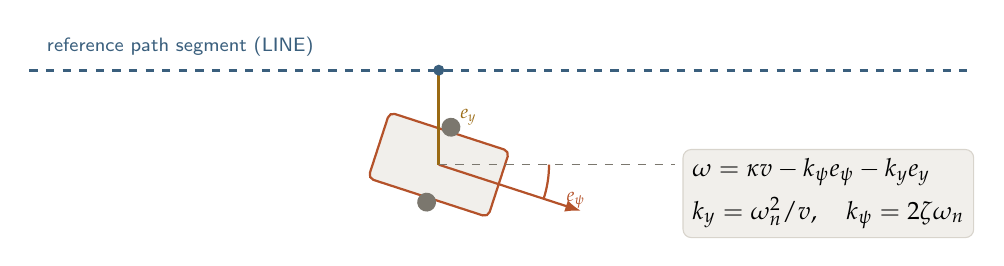
\begin{tikzpicture}[scale=1]
  \draw[cold,very thick,dashed] (0,2.6) -- (12,2.6);
  \node[lbl,text=cold,anchor=west] at (0.1,2.9) {reference path segment (LINE)};
  \begin{scope}[shift={(5.2,1.4)},rotate=-18]
    \draw[draw=accent,fill=greybg,thick,rounded corners=2pt] (-0.8,-0.44) rectangle (0.8,0.44);
    \fill[grey] (0,0.5) circle (0.12); \fill[grey] (0,-0.5) circle (0.12);
    \draw[-{Latex[length=2mm]},accent,thick] (0,0) -- (1.9,0);
  \end{scope}
  \draw[warn,very thick] (5.2,2.6) -- (5.2,1.4);
  \node[lbl,text=warn,anchor=west] at (5.35,2.0) {$e_y$};
  \fill[cold] (5.2,2.6) circle (0.07);
  \draw[grey,thin,dashed] (5.2,1.4) -- (8.2,1.4);
  \draw[accent,thick] (6.6,1.4) arc (0:-18:1.4);
  \node[lbl,text=accent,anchor=west] at (6.7,0.95) {$e_\psi$};
  \node[draw=rule,fill=greybg,rounded corners=3pt,anchor=north east,align=left,font=\small] at (12,1.6)
       {$\omega=\kappa v-k_\psi e_\psi-k_y e_y$\\[1mm]
        $k_y=\omega_n^2/v,\quad k_\psi=2\zeta\omega_n$};
\end{tikzpicture}
\caption{Cross-track error $e_y$ (signed, left of the path positive) and heading
error $e_\psi=\theta-\theta_{path}$. The feedforward $\kappa v$ follows the
path curvature; the feedback is a linear second-order design.}
\label{fig:pathfollow}
\end{figure}

\paragraph{Linear cross-track/heading controller (recommended).} Relative to a
path of curvature $\kappa$ the error kinematics are
$\dot e_y=v\sin e_\psi$, $\dot e_\psi=\omega-\kappa v$. With
$\omega=\kappa v-k_\psi e_\psi-k_y e_y$ and small angles,
\begin{equation}
\ddot e_y+k_\psi\,\dot e_y+k_y v\,e_y=0
\quad\Rightarrow\quad
\omega_n^2=k_y v,\qquad 2\zeta\omega_n=k_\psi .
\end{equation}
Scheduling $k_y=\omega_n^2/v$ keeps the dynamics independent of speed (in
distance terms the convergence then shortens at low speed --- acceptable, because
slow driving only happens in approaches). \textbf{Bandwidth choice:} the speed
loop closes at $\omega_c=\qty{6.8}{rad/s}$ and the wheel position loop at
\qty{2}{rad/s}; with a factor of 3--5 separation the path loop should use
$\omega_n\approx\qtyrange{1.5}{2}{rad/s}$, $\zeta=0.7$, i.e.\
$k_\psi=\qtyrange{2.1}{2.8}{s^{-1}}$ and $k_y=\qtyrange{7.5}{13.3}{m^{-1}s^{-1}}$
at \qty{0.3}{m/s}. (The earlier concept figure of ``about 1\,Hz'' bandwidth,
\qty{6.3}{rad/s}, would sit on top of the speed loop and is corrected here.) The
command is limited so that neither wheel set-point
$v\pm\omega b/2$ exceeds the speed ceiling; if it would, $v$ is reduced and
$\omega$ kept.

\paragraph{Pure Pursuit (alternative).} Steer towards a look-ahead point at
distance $L_d$: $\kappa=2y_L/L_d^2$ ($y_L$ lateral offset of that point in the
body frame), $\omega=\kappa v$, $L_d=L_0+k v$. Robust with one parameter, but it
cuts corners systematically; kept as fallback.

\paragraph{TURN primitive.} Corners are driven as stop--turn--go. The turn
follows a trapezoidal angle profile $\theta_{ref}(t)$ with
$\omega_{cmd}=\dot\theta_{ref}+K_\theta(\theta_{ref}-\hat\theta)$ on the gyro
heading, wheel set-points $\pm\omega_{cmd}b/2$, $K_\theta\approx\qty{2}{s^{-1}}$;
termination on $|\theta_{ref,end}-\hat\theta|<\ang{0.2}$ and $|\omega|$ small,
approaching from one direction only. Turn in place is the cleanest manoeuvre of a
differential drive: ICR at the axle midpoint, no lateral tyre forces, best gyro
accuracy (pure yaw).

\paragraph{Mapping onto the present firmware.} A \code{LINE} of known length maps
onto today's \code{D<mm>} cascade with the path follower's $\omega$ added as a
differential speed $\pm\omega b/2$ to $v_{cmd,L/R}$; a \code{TURN} maps onto a
distance move with opposite signs, $D_{L,R}=\mp\Delta\theta\,b/2$, corrected by the
gyro. This reuses the tested wheel cascade instead of replacing it.

% ---------------------------------------------------------------------
\subsection{Mission logic}\label{sec:mission}

\begin{figure}[htbp]
\centering
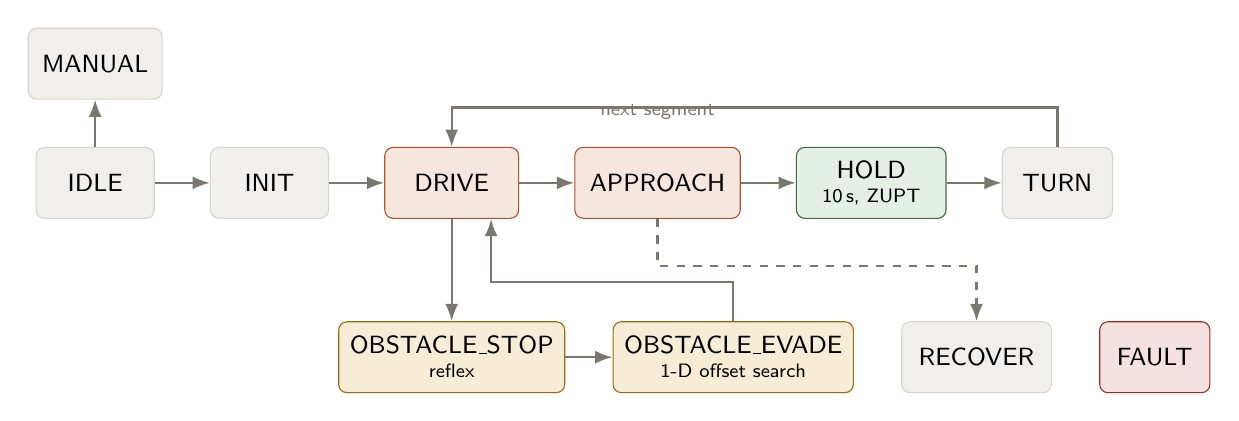
\begin{tikzpicture}[node distance=7mm]
  \node[blk,minimum width=15mm] (idle) {IDLE};
  \node[blk,minimum width=17mm,above=6mm of idle] (man) {MANUAL};
  \node[blk,minimum width=15mm,right=7mm of idle] (init) {INIT};
  \node[blkA,minimum width=17mm,right=7mm of init] (drive) {DRIVE};
  \node[blkA,minimum width=21mm,right=7mm of drive] (appr) {APPROACH};
  \node[blkG,minimum width=19mm,right=7mm of appr] (hold) {HOLD\\[-0.8mm]{\scriptsize 10\,s, ZUPT}};
  \node[blk,minimum width=14mm,right=7mm of hold] (turn) {TURN};
  \draw[arr] (idle) -- (man);
  \draw[arr] (idle) -- (init);
  \draw[arr] (init) -- (drive);
  \draw[arr] (drive) -- (appr);
  \draw[arr] (appr) -- (hold);
  \draw[arr] (hold) -- (turn);
  \draw[arr] (turn.north) -- ++(0,5mm) -| (drive.north);
  \node[lbl] at ($(appr)+(0,9mm)$) {next segment};
  \node[blkW,minimum width=26mm,below=13mm of drive] (ostop) {OBSTACLE\_STOP\\[-0.8mm]{\scriptsize reflex}};
  \node[blkW,minimum width=26mm,right=6mm of ostop] (oev) {OBSTACLE\_EVADE\\[-0.8mm]{\scriptsize 1-D offset search}};
  \node[blk,minimum width=19mm,right=6mm of oev] (rec) {RECOVER};
  \node[blkB,minimum width=14mm,right=6mm of rec] (fault) {FAULT};
  \draw[arr] (drive) -- (ostop);
  \draw[arr] (ostop) -- (oev);
  \draw[arr] (oev.north) -- ++(0,5mm) -| ($(drive.south)+(5mm,0)$);
  \draw[arr,dashed] (appr.south) -- ++(0,-6mm) -| (rec.north);
\end{tikzpicture}
\caption{Mission state machine. Each state has entry, cycle and exit actions and
an explicit table of allowed transitions; no nested if-cascades.}
\label{fig:fsm}
\end{figure}

\begin{center}
\small
\begin{tabularx}{\textwidth}{@{}lL@{}}
\toprule
\textbf{Transition} & \textbf{Guard and rationale}\\
\midrule
INIT $\to$ DRIVE & gyro bias variance $P_{b_g}$ below threshold (not a fixed timeout); battery above cut-off; all sensors alive\\
DRIVE $\to$ APPROACH & along-track distance to the waypoint $<s_{appr}$ (\qty{1}{m}) \textbf{and} $|y_{offset}|<\qty{0.05}{m}$: an unfinished evasion keeps the vehicle in DRIVE --- seconds are free, centimetres are graded\\
APPROACH $\to$ HOLD & $|e_s|<\qty{2}{mm}$ in the encoder frame and speed zero; approach at \qty{0.1}{m/s}, always ending forward\\
HOLD $\to$ TURN & \qty{10}{s} elapsed (timed from standstill, with margin \qty{0.5}{s}); ZUPT applied; bias updated\\
any $\to$ OBSTACLE\_STOP & forward range below the stopping distance --- issued by the reflex layer, not by this machine\\
OBSTACLE\_STOP $\to$ EVADE & obstacle persists beyond a wait time (temporary obstacles are waited out: 1 point; rerouting: 2 points)\\
any $\to$ RECOVER & reference lost too long, or $\operatorname{tr}P$ above a bound; slow down, seek the edge\\
any $\to$ FAULT & stall, battery cut-off, sensor timeout, inner ground sensor sees drop/grass\\
\bottomrule
\end{tabularx}
\end{center}

\subsection{Safety and failsafe}\label{sec:safety}

\begin{center}
\small
\begin{tabularx}{\textwidth}{@{}lLc@{}}
\toprule
\textbf{Mechanism} & \textbf{Behaviour} & \textbf{State}\\
\midrule
EN pull-downs & internal + \qty{10}{k\ohm} external: drivers off during reset and before init & \tg{done}\\
Single setter & forbidden output combinations unreachable by construction & \tg{done}\\
Stall detection & bench: $|d|>15\,\%$, $<\qty{5}{rpm}$, \qty{300}{ms}; calibration: $|d|\ge0.30$, $<\qty{0.5}{rpm}$, \qty{0.5}{s}; \textbf{suspended} during deliberate-stall measurements & \tg{done}\\
Wheel fault & position error persists \qty{0.6}{s} (30 ticks) $\to$ stop & \tg{done}\\
Dead-man & no input for \qty{2}{s} in open-loop/manual $\to$ stop & \tg{done}\\
Tracking/excursion abort & calibration: tracking error $>\qty{40}{mm}$, L/R difference $>\qty{30}{mm}$ & \tg{done}\\
Radio heartbeat & manual mode: no valid command for \qty{500}{ms} $\to$ $v_{ref}=0$ & \tk{planned}\\
Battery cut-off & \qty{10.0}{V}, plus independent LiPo alarm on the balance lead & \tw{divider missing}\\
Error\_Handler & CCR1--4 $=0$, EN low before looping & \tw{O-12}\\
IWDG & LSI \qty{32}{kHz}, prescaler 32, reload 100 $\Rightarrow$ \qty{100}{ms}; frozen in debug (\code{\_\_HAL\_DBGMCU\_FREEZE\_IWDG}) & \tk{planned}\\
CSS & clock failure $\to$ HSI + NMI; NMI handler stops the motors & \tk{planned}\\
Reflex stop & forward VL53L1X, highest priority, bypasses planning & \tk{planned}\\
Inner ground interlock & inner downward sensor sees drop/grass $\to$ stop; never disabled, not even during evasion & \tk{planned}\\
Hardware kill & \textbf{possible now}: EN lines are separate from PWM on the BTS7960, so a mechanical E-stop in series with EN (or the main switch) gives a firmware-independent stop \DECIDE & \tk{proposal}\\
\bottomrule
\end{tabularx}
\end{center}

\begin{warnbox}
\textbf{Lesson from the bench.} The stall supervisor aborted the deadband sweep,
because a stationary shaft above the duty threshold \emph{is} the measurement
there. A safety mechanism and a measurement procedure contradicted each other.
Every new sequence that deliberately stalls a wheel (breakaway test, pushing
against a kerb on purpose) must re-examine the stall rule's scope.
\end{warnbox}
% =====================================================================
\clearpage
\section{State estimation}\label{sec:ekf}

The controller can hold a position to a few millimetres in its \emph{own}
frame; the graded quantity is where the vehicle really is. The accuracy grade
therefore rides on the estimate, not on the controller. The estimator is a
five-state Extended Kalman Filter running at \qty{200}{Hz} \OPEN.

\subsection{State and process model}

\begin{equation}
\vect x=\begin{bmatrix}x & y & \theta & b_g & s\end{bmatrix}\T
\end{equation}
\begin{center}
\small
\begin{tabularx}{\textwidth}{@{}llL@{}}
\toprule
\textbf{State} & \textbf{Meaning} & \textbf{Why it is estimated}\\
\midrule
$x,\,y$ & position of the axle midpoint in $\{W\}$ & the graded quantity\\
$\theta$ & heading & drives all position integration\\
$b_g$ & gyro bias & drifts with temperature; integrates directly into heading error\\
$s$ & odometry scale factor ($\approx1$) & largest along-track error; changes with load, tyre and surface\\
\bottomrule
\end{tabularx}
\end{center}

\textbf{Inputs} per step $\Delta t$: the encoder distance
$\Delta s_e=\tfrac12(\Delta s_L+\Delta s_R)$ with nominal distance per count, and
the mean gyro rate $\omega_m$ over the step. Heading comes from the gyro; the
wheel difference is used only by the slip detector.
\begin{equation}
\begin{aligned}
\varphi &= \theta+\tfrac12(\omega_m-b_g)\Delta t, & \Delta s &= s\,\Delta s_e,\\
x^+ &= x+\Delta s\cos\varphi, & y^+ &= y+\Delta s\sin\varphi,\\
\theta^+ &= \theta+(\omega_m-b_g)\Delta t, & b_g^+ &= b_g,\quad s^+=s .
\end{aligned}\label{eq:ekfpred}
\end{equation}
Bias and scale are random walks. Jacobians with respect to the state and to the
inputs $(\Delta s_e,\omega_m)$, using $c_\varphi=\cos\varphi$, $s_\varphi=\sin\varphi$:
\begin{equation}
F=\begin{bmatrix}
1&0&-\Delta s\,s_\varphi & \tfrac12\Delta s\,s_\varphi\Delta t & \Delta s_e c_\varphi\\
0&1&\Delta s\,c_\varphi & -\tfrac12\Delta s\,c_\varphi\Delta t & \Delta s_e s_\varphi\\
0&0&1&-\Delta t&0\\
0&0&0&1&0\\
0&0&0&0&1
\end{bmatrix},\qquad
G=\begin{bmatrix}
s\,c_\varphi & -\tfrac12\Delta s\,s_\varphi\Delta t\\
s\,s_\varphi & \tfrac12\Delta s\,c_\varphi\Delta t\\
0&\Delta t\\ 0&0\\ 0&0
\end{bmatrix}
\end{equation}
\begin{equation}
P^+=F P F\T + G M G\T + Q_{rw},\qquad
M=\diag\bigl(k_d|\Delta s_e|,\ \sigma_\omega^2\bigr),\qquad
Q_{rw}=\diag\bigl(0,0,0,\ q_b\Delta t,\ q_s\Delta t\bigr).
\end{equation}
The distance noise grows with distance travelled ($k_d$, from repeated
straight runs); $\sigma_\omega$, $q_b$ come from the IMU's Allan variance (angle
random walk and bias instability); $q_s$ is small (the scale changes with
surface, not with time).

\paragraph{Slip detection.} The encoder yaw rate
$\omega_e=(\Delta s_R-\Delta s_L)/(b\,\Delta t)$ is compared with the gyro,
$r_{slip}=\omega_e-(\omega_m-b_g)$. If $|r_{slip}|$ exceeds a threshold for
several samples (wheel spin, a caster dropping off an edge), $k_d$ is inflated
for those samples: the filter trusts the encoders less exactly when they lie.
It costs nothing and uses sensors that are already there.

\subsection{Measurement models}\label{sec:meas}

All updates are scalar or 2-D and are processed sequentially, so no matrix
inversion is needed. Sensor positions on the body are $\vect r_s$ (mounting
point) and $\vect u_s$ (unit viewing direction); $R(\theta)$ is the 2-D rotation
and $R'(\theta)=\mathrm dR/\mathrm d\theta$.

\begin{center}
\small
\begin{tabularx}{\textwidth}{@{}lp{40mm}p{37mm}L@{}}
\toprule
\textbf{Type} & \textbf{Model $h(\vect x)$} & \textbf{$H$ (non-zero)} & \textbf{When / noise}\\
\midrule
ZUPT & $h=b_g$, $z=\overline{\omega_m}$ over the stop & $H_{b_g}=1$ & every stop $\geq\qty{1}{s}$; $R=\sigma_\omega^2/N$\\
Edge crossing & $h=\vect n\T(\vect p+R(\theta)\vect r_s)-d_e$, $z=0$ & $\vect n\T$; $\vect n\T R'\vect r_s$ & downward sensor changes class (path/edge/grass); $\sigma\approx\qty{2}{cm}$ (spot)\\
Range to a face & $h=\dfrac{d_f-\vect n\T(\vect p+R\vect r_s)}{\vect n\T R\,\vect u_s}$ & $-\vect n\T/g$; $\partial h/\partial\theta$ & lateral sensor along a mapped straight face; $g=\vect n\T R\vect u_s$\\
Face heading & $h=\theta$, $z=\psi_{face}+\Delta\hat\psi$ & $H_\theta=1$ & after a line fit over $\geq\qty{1}{m}$; $\sigma$ from \cref{eq:headingfit}\\
Landmark (post) & $h=\vect p+R(\theta)(\vect r_s+r\,\vect u_s)$, $z=\vect p_L$ & $I_2$; $R'(\vect r_s+r\vect u_s)$ & notch centre in the lateral range profile; 2-D, makes $s$ observable\\
\bottomrule
\end{tabularx}
\end{center}

\paragraph{About the non-holonomic constraint.} The concept lists NHC (zero
lateral body velocity, \cref{eq:nhc}) as a measurement type. In this five-state
model the prediction \cref{eq:ekfpred} moves the vehicle only along its heading,
so NHC is \emph{already built into the process model} and adds no information as
a separate update. It becomes a genuine pseudo-measurement only if the state is
extended by velocity or a lateral slip state (e.g.\ for accelerometer-aided
prediction). The listing is kept for completeness; no update code is needed for
it now.

\paragraph{Update.} $\nu=z-h(\hat{\vect x})$, $S=HPH\T+R$, $K=PH\T S^{-1}$,
$\hat{\vect x}\mathrel{+}=K\nu$, and the covariance in Joseph form
\begin{equation}
P=(I-KH)P(I-KH)\T+KRK\T,
\end{equation}
because the short form $(I-KH)P$ loses symmetry and positive definiteness in
single precision --- the F446 has a single-precision FPU only.

\paragraph{Outlier gate.} Every update is gated on the Mahalanobis distance
$d^2=\nu\T S^{-1}\nu$: reject if $d^2>9$ for a scalar ($\chi^2_1$, 99.7\,\%)
or $d^2>9.2$ for 2-D ($\chi^2_2$, 99\,\%). A false edge detection or another
vehicle standing where a landmark is expected would otherwise wrench the
filter. \textbf{The gate is present from the first line of code.} Landmark and
face updates are additionally suppressed while an evasion offset
$|y_{offset}|>\qty{0.1}{m}$ is active.

\paragraph{Timing.} Every measurement carries the timestamp of its physical
acquisition from the \qty{1}{MHz} time base: IMU by input capture of DRDY, VL53L1X
at the middle of the integration window. Measurements older than the current
state are applied with the state from a short history buffer (\qty{100}{ms}),
or --- for latencies below one EKF step --- simply at the next step. Load: a
five-state EKF at \qty{200}{Hz} costs well under \qty{1}{\percent} of the CPU.

\paragraph{Initialisation.} INIT stands still until the variance of $b_g$ has
converged; $x,y,\theta$ are zero by definition (start mark and start heading
define $\{W\}$); $s=1$ with the variance of the scale calibration. The start
heading must therefore be set physically: a jig or two marks on the ground at
the start position \DECIDE.

\subsection{Observability}\label{sec:observability}

\begin{center}
\small
\begin{tabular}{@{}lll@{}}
\toprule
\textbf{Configuration} & \textbf{Observable} & \textbf{Not observable}\\
\midrule
Dead reckoning only & nothing absolute & $x,y,\theta$ drift; $s$ never\\
+ ZUPT & $b_g$ & position, heading, $s$\\
+ lateral edge & position \emph{perpendicular} to the edge & position along the edge\\
+ straight-face fit & heading, absolutely & ---\\
+ longitudinal landmark & position along travel, hence $s$ & ---\\
\bottomrule
\end{tabular}
\end{center}

\begin{goodbox}
\textbf{Flat surfaces give heading; round objects give position.} A post looks
the same from every direction: a full 2-D position fix, no heading. A bench face
gives heading to a fraction of a degree, but only a weak position fix. \textbf{Corners
rotate the observable direction:} on a north-going segment the edge constrains
$x$; after a \ang{90} turn the same kind of edge constrains $y$ --- precisely the
error that accumulated unobserved before. Over the circuit the full 2-D position
becomes observable without any absolute position sensor; the course geometry does
it.
\end{goodbox}

\subsection{IMU integration}\label{sec:imu}

\begin{itemize}[leftmargin=6mm]
\item \textbf{Selection.} ICM-42688-P unobtainable; \textbf{ISM330DHCX}
(Adafruit breakout) selected. Criteria in
order: gyro temperature-offset stability, noise density, SPI for DMA, a data-ready
output for hardware timestamping, local availability. MPU-6050/9250 and
ICM-20948 only as bring-up placeholders (poor temperature stability,
discontinued, counterfeit-prone).
\item \textbf{Interface.} SPI1 (PB3/PB4/PB5, CS PA4), \qty{5.625}{MHz} (APB2/16; the ISM330DHCX allows at most \qty{10}{MHz}); DRDY
on PA1 = TIM2\_CH2 input capture gives a jitter-free timestamp; the capture
interrupt starts the DMA read. The ISM330DHCX has no \qty{1}{kHz} output data rate: sample at \qty{833}{Hz} with the sensor's
anti-aliasing filter and decimate by 4 to $\approx\qty{208}{Hz}$ for the \qty{200}{Hz} EKF \VERIFY\ (datasheet ODR table).
\item \textbf{Mounting.} Rigid, at the axle midpoint (no lever-arm accelerations
in turns), not soft-mounted (an elastic mount creates a resonance in the band of
interest), thermally away from the drivers, under a light-coloured cover.
\item \textbf{Temperature.} Outdoors the die temperature may move
\qtyrange{20}{30}{K} during a run. Second-order polynomial bias model against the
internal temperature sensor from a calibration run; \qty{10}{min} warm-up before
runs; ZUPT at every stop removes the residual.
\end{itemize}
% =====================================================================
\clearpage
\section{Lateral aiding and boundary sensing}\label{sec:lateral}

Lateral aiding (cross-track support) is the use of the path's own boundaries ---
grass edge, rubber edging, kerb, step, benches --- as a continuous reference
that bounds the cross-track error independently of how far the vehicle has
driven. Dead reckoning drifts without bound; a boundary measurement does not.

\subsection{Sensor layout and roles}

\begin{figure}[htbp]
\centering
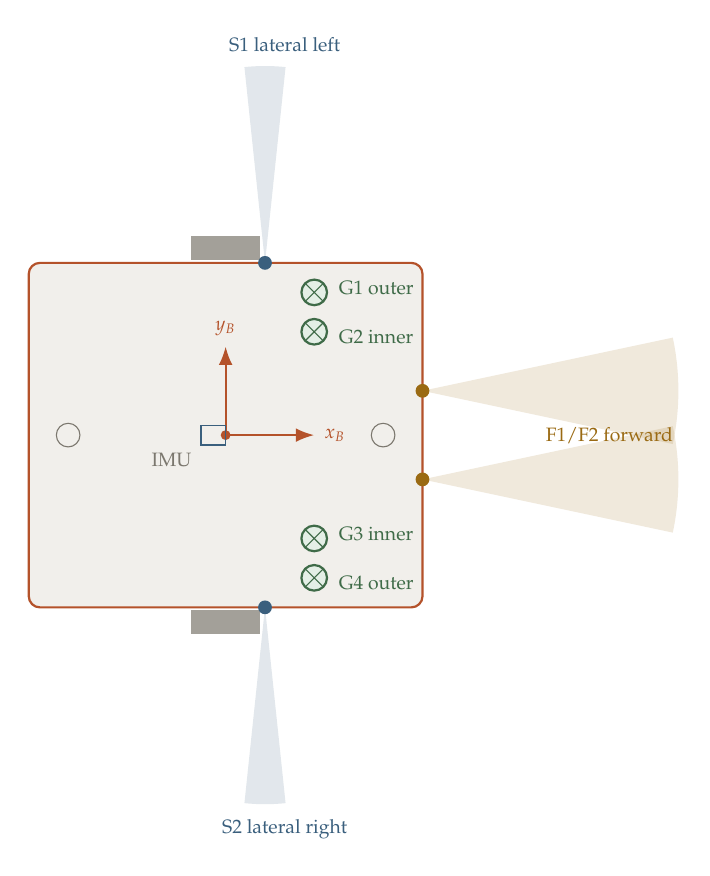
\begin{tikzpicture}[scale=1.25]
  % chassis
  \draw[draw=accent,fill=greybg,thick,rounded corners=4pt] (-2.0,-1.75) rectangle (2.0,1.75);
  \fill[grey!70] (-0.35,1.78) rectangle (0.35,2.02);
  \fill[grey!70] (-0.35,-2.02) rectangle (0.35,-1.78);
  \draw[grey] (1.6,0) circle (0.12); \draw[grey] (-1.6,0) circle (0.12);
  \draw[-{Latex},accent,thick] (0,0) -- (0.9,0) node[right,font=\scriptsize] {$x_B$};
  \draw[-{Latex},accent,thick] (0,0) -- (0,0.9) node[above,font=\scriptsize] {$y_B$};
  \fill[accent] (0,0) circle (0.05);
  \node[font=\scriptsize,grey] at (-0.55,-0.25) {IMU};
  \draw[cold] (-0.25,-0.1) rectangle (0.0,0.1);
  % ground sensors (down) - circles with cross
  \foreach \p/\l in {(0.9,1.45)/G1,(0.9,1.05)/G2,(0.9,-1.45)/G4,(0.9,-1.05)/G3}{
    \draw[good,thick,fill=goodbg] \p circle (0.13);
    \draw[good] \p ++(-0.09,-0.09) -- ++(0.18,0.18) \p ++(-0.09,0.09) -- ++(0.18,-0.18);
  }
  \node[font=\scriptsize,good,anchor=west] at (1.05,1.5) {G1 outer};
  \node[font=\scriptsize,good,anchor=west] at (1.05,1.0) {G2 inner};
  \node[font=\scriptsize,good,anchor=west] at (1.05,-1.0) {G3 inner};
  \node[font=\scriptsize,good,anchor=west] at (1.05,-1.5) {G4 outer};
  % forward
  \foreach \yy in {0.45,-0.45}{
    \fill[warn] (2.0,\yy) circle (0.07);
    \fill[warn,opacity=0.15] (2.0,\yy) -- ++(12:2.6) arc (12:-12:2.6) -- cycle;
  }
  \node[font=\scriptsize,warn] at (3.9,0) {F1/F2 forward};
  % lateral
  \fill[cold] (0.4,1.75) circle (0.07);
  \fill[cold,opacity=0.15] (0.4,1.75) -- ++(96:2.0) arc (96:84:2.0) -- cycle;
  \node[font=\scriptsize,cold,anchor=south] at (0.6,3.8) {S1 lateral left};
  \fill[cold] (0.4,-1.75) circle (0.07);
  \fill[cold,opacity=0.15] (0.4,-1.75) -- ++(-96:2.0) arc (-96:-84:2.0) -- cycle;
  \node[font=\scriptsize,cold,anchor=north] at (0.6,-3.8) {S2 lateral right};
\end{tikzpicture}
\caption{Planned sensor layout (top view, not to scale). Ground sensors G1--G4
look straight down, two per side at different lateral offsets (e.g.\ 15 and
\qty{25}{cm} from the centre line) \DECIDE. Forward sensors F1/F2 serve the
reflex layer and free-space estimation; lateral sensors S1/S2 look sideways at
benches, posts and kerbs. G on I2C1, F and S on I2C2; every sensor has its own
XSHUT line. Only five VL53L1X were ordered (four fitted, one spare): G1--G4
are fitted, F1/F2 and S1/S2 are not covered \DECIDE.}
\label{fig:layout}
\end{figure}

The four ground sensors have four distinct roles that are easy to conflate:

\begin{center}
\small
\begin{tabularx}{\textwidth}{@{}clL@{}}
\toprule
\# & \textbf{Role} & \textbf{What it protects}\\
\midrule
1 & Run validity & a circuit that touches grass is invalid --- lost as a whole, not gradually\\
2 & Physical safety & kerbs and the step are drop-offs; driving off ends the run and may damage the vehicle\\
3 & EKF measurement & edge updates make the position perpendicular to the edge observable (\cref{sec:observability})\\
4 & Evasion bound & the lateral search range ends at the \emph{detected} edge, not the estimated one (\cref{sec:evasion})\\
\bottomrule
\end{tabularx}
\end{center}

No horizontal sensor can take these over: a \qtyrange{3}{4}{cm} rubber edging,
an \qty{8}{cm} kerb or a flush grass transition is invisible to a sensor
mounted \qtyrange{25}{35}{cm} high and looking horizontally.

\subsection{Three-valued edge state}

\begin{center}
\small
\begin{tabular}{@{}lll@{}}
\toprule
\textbf{Inner sensor} & \textbf{Outer sensor} & \textbf{Meaning}\\
\midrule
path & path & edge further out than the outer sensor --- drift away is allowed up to the corridor model\\
path & edge/drop/grass & edge between the two sensors --- \textbf{nominal}, cross-track known to $\approx\qty{\pm5}{cm}$\\
edge/drop/grass & any & edge too close --- \textbf{emergency stop}\\
\bottomrule
\end{tabular}
\end{center}

During an evasion the vehicle deliberately approaches an edge: the
\textbf{outer} sensor is then the operating signal that bounds the offset; the
\textbf{inner} sensor is the interlock and is \textbf{never disabled}. A
planner that commands an offset which trips the inner sensor has a fault, not a
manoeuvre. This is why both pairs are needed from the first autonomous build.

\subsection{Classification of path, edge and grass}

Each reading delivers range $r$, signal rate $S$ and sigma $\sigma$. With a
mounting height $h_0$ over paving:
\begin{itemize}[leftmargin=6mm]
\item \textbf{Drop/step down}: $r>h_0+\Delta_{min}$ (kerb \qty{8}{cm}, step);
\item \textbf{Edging/step up}: $r<h_0-\Delta_{min}$ with low $\sigma$;
\item \textbf{Grass}: $r$ noisy and short (blades above ground), high $\sigma$,
low $S$;
\item \textbf{Paving}: $r\approx h_0$, low $\sigma$, high $S$.
\end{itemize}
A debounce of 2--3 consecutive samples suppresses single leaves or cracks; a
transition is time-stamped at the middle of the integration window of the first
sample in the new class. \MEASURE\ thresholds $\Delta_{min}$, $\sigma$ and $S$ on
the actual surfaces at noon and in the afternoon (sunlight raises the ambient
rate and $\sigma$).

\subsection{Cross-track correction}

Two forms are used, depending on the boundary:

\begin{enumerate}[leftmargin=6mm]
\item \textbf{Edge crossing events} (ground sensors). Each class change of a
sensor places its footprint on the mapped boundary line; the EKF receives the
constraint $\vect n\T(\vect p+R(\theta)\vect r_s)=d_e$
(\cref{sec:meas}). With the vehicle driving along the edge, the outer sensor
toggles intermittently as it skims the edge, which gives a stream of fixes.
Accuracy is set by the footprint (\qtyrange{5}{8}{cm} at ROI $4\times4$,
\cref{sec:tofmodel}), $\sigma\approx\qty{2}{cm}$.
\item \textbf{Continuous range} (lateral sensors) to a face of known position:
kerb face, bench face, wall. Gives cross-track continuously and, via the line
fit (\cref{eq:headingfit}), absolute heading.
\end{enumerate}

\begin{keybox}
\textbf{Why the boundary matters more than any other aid.} The entry heading
error at the start of a reference-free segment dominates the error budget
(\cref{sec:budget}); a boundary bounds cross-track drift wherever it exists, and
a straight face resets heading. The path is in effect a rail: the edge is a free
measurement that is always present unless the vehicle is in an evasion or the
boundary has a gap. Reference-free stretches immediately before waypoints are
therefore the decisive survey item \MEASURE.
\end{keybox}

\subsection{Landmarks for along-track position}

Along a straight edge, position \emph{along} the edge is unobservable. It is
supplied by discrete landmarks: posts (2-D fix via the notch centre), the ends
of benches and tables, the beginning or end of an edging, path junctions (edge
appears or disappears on one side), and the step (also detectable as an IMU
impulse if crossed). The landmark map is a survey product: positions to
$\pm\qty{5}{cm}$, face orientations to $\pm\ang{0.5}$ \MEASURE. Furniture may be
moved before the exam day \ASK; landmark updates are gated and optional by
design.

\subsection{Bus and timing}

\begin{itemize}[leftmargin=6mm]
\item Four sensors per bus at \qty{400}{kHz}; a timing budget of \qty{20}{ms}
gives \qty{50}{Hz} per sensor; with the Ultra Lite Driver each readout is a few
dozen bytes, bus load $\approx\qty{15}{\percent}$.
\item Start-up: all XSHUT low, then release one at a time and assign a new address.
\item One hung device blocks a bus: per-transaction timeouts and a bus recovery
(nine clock pulses, STOP). Ground and horizontal sensors on separate buses so
that one failure does not take out edge \emph{and} obstacle detection.
\item The two forward sensors start with a time offset so that their emitters
do not disturb each other where the fields of view overlap.
\item \RISK\ Outdoor range: short mode is nominally \qty{1.3}{m}, at noon in
sun less. For the reflex stop \qty{0.5}{m} suffice; for evasion planning the
vehicle slows to \qty{0.25}{m/s} when an object is in view.
\end{itemize}
% =====================================================================
\clearpage
\section{Path planning}\label{sec:planning}

\subsection{Course representation}

The course is known in advance; planning is therefore an \emph{offline}
geometric task done once from the survey, plus an \emph{online} 1-D lateral
re-planning for obstacles. The path is a list of primitives in $\{W\}$:
\begin{center}
\ttfamily\small
\{ LINE($\vect p_1,\vect p_2$) | ARC($\vect c, r, \varphi_1, \varphi_2$) | TURN($\theta_{target}$) | PAUSE($t$) | WAYPOINT($id$) \}
\end{center}
Each segment also carries its \textbf{corridor} (signed distances from the path
line to the left and right boundaries, boundary type per side), its
\textbf{speed limit}, and the \textbf{landmarks} visible from it. A plain
polyline through the waypoints is not used: its curvature jumps at every vertex
would demand infinite $\omega$.

\subsection{Route}

From the schematic (\cref{fig:course}), clockwise around the central green:

\begin{center}
\small
\begin{tabularx}{\textwidth}{@{}clLl@{}}
\toprule
\textbf{Leg} & \textbf{From $\to$ to} & \textbf{Character} & \textbf{Length}\\
\midrule
1 & X $\to$ WP1 (south) & diagonal path south-west, then west into the waypoint & \MEASURE\\
2 & WP1 $\to$ WP2 (north-west) & long straight northbound path on the western side --- probably the longest reference segment & \MEASURE\\
3 & WP2 $\to$ corner north-east & eastbound along the northern path, step running parallel on the north side & \MEASURE\\
4 & corner $\to$ WP3 (north-east) & short south-east leg & \MEASURE\\
5 & WP3 $\to$ X & south, then diagonal south-west back to the start; the barrier lies south-east of X & \MEASURE\\
\bottomrule
\end{tabularx}
\end{center}

Total length $\approx\qty{150}{m}$ (estimate from the concept; \MEASURE). Corners
between legs are driven as stop--\code{TURN}--go on level ground; \code{ARC} only
where the path itself is curved.

\subsection{Speed profile and time budget}\label{sec:timebudget}

\begin{center}
\small
\begin{tabular}{@{}lccccc@{}}
\toprule
\textbf{Cruise speed} & 0.20 & 0.25 & 0.30 & 0.40 & m/s\\
\midrule
Driving time for 150\,m & 750 & 600 & 500 & 375 & s\\
+ 3 waypoint stops (\qty{10}{s}) & 780 & 630 & 530 & 405 & s\\
Reserve to \qty{15}{min} (turns, approaches, obstacles) & 120 & 270 & 370 & 495 & s\\
\bottomrule
\end{tabular}
\end{center}

Recommended: cruise \qty{0.3}{m/s}, \qty{0.25}{m/s} when an object is in the
forward field, \qty{0.1}{m/s} over the last metre to a waypoint, accelerations
$\leq\qty{0.3}{m/s^2}$. This leaves about 6 minutes for turns, slow approaches,
INIT and waiting out obstacles. Driving faster earns nothing and costs accuracy
(scale error grows with slip; transients grow with acceleration).

\subsection{Waypoint approach and hold}

Waypoint accuracy is made in the last metre, not by the path follower:
\begin{enumerate}[leftmargin=6mm]
\item Before the waypoint, use the last reliable references: a landmark fix for
along-track, the edge or a face fit for cross-track and heading.
\item \code{APPROACH} at \qty{0.1}{m/s} with the Coulomb feedforward active (the
weaker wheel breaks away near the approach duty), deceleration ending forward,
no reversal.
\item Stop on the EKF estimate of the waypoint position; hold \qty{10}{s} plus a
margin, apply ZUPT (bias reset for the next leg).
\item If an obstacle stands on the waypoint: wait; if it persists, approach as
close as clearance allows and hold there --- a lower accuracy grade beats a
missed stop.
\end{enumerate}

\subsection{Turning near ramps}

The concept documents a ramp on the circuit (lip height and gradient
unmeasured). Turning on a slope corrupts the heading (\cref{eq:euler}). Sequence:
(1) approach perpendicular to the sidewalk axis; (2) drive until all four wheels
are on the flat; (3) stop; (4) ZUPT and pitch check; (5) turn in place by
\ang{90}; (6) drive \qtyrange{20}{30}{cm} straight to align the casters;
(7) re-acquire the edge. If the sidewalk at the ramp entry is narrower than the
\qty{0.6}{m} turning envelope, the turn happens on the slope: slope projection
becomes mandatory and the turn is split into two \ang{45} steps \MEASURE.

\subsection{Obstacle handling as a one-dimensional problem}\label{sec:evasion}

The vehicle drives in a corridor whose boundaries it measures. Evasion is
therefore not 2-D planning: the single free variable is the lateral offset
$y_{off}$ from the nominal path within the corridor.

\begin{figure}[htbp]
\centering
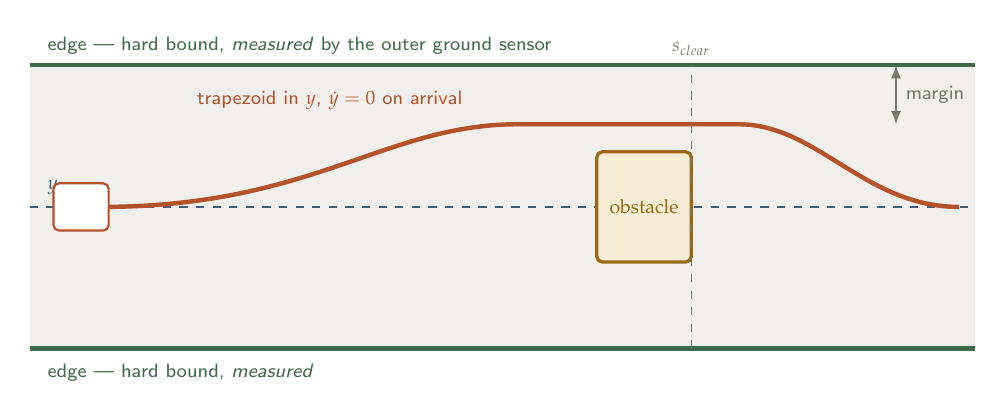
\begin{tikzpicture}[yscale=1.0]
  \fill[greybg] (0,0) rectangle (12,3.6);
  \draw[good,ultra thick] (0,3.6) -- (12,3.6);
  \draw[good,ultra thick] (0,0) -- (12,0);
  \node[lbl,text=good,anchor=west] at (0.1,3.85) {edge --- hard bound, \emph{measured} by the outer ground sensor};
  \node[lbl,text=good,anchor=west] at (0.1,-0.3) {edge --- hard bound, \emph{measured}};
  \draw[cold,thick,dashed] (0,1.8) -- (12,1.8);
  \node[lbl,text=cold,anchor=west] at (0.1,2.05) {$y_{nom}$};
  \draw[warn,very thick,fill=warnbg,rounded corners=2pt] (7.2,1.1) rectangle (8.4,2.5);
  \node[font=\scriptsize\color{warn}] at (7.8,1.8) {obstacle};
  \draw[accent,ultra thick] (0.9,1.8) .. controls (3.6,1.8) and (4.5,2.85) .. (6.2,2.85) -- (9.0,2.85)
        .. controls (10.0,2.85) and (10.6,1.8) .. (11.8,1.8);
  \draw[draw=accent,fill=white,thick,rounded corners=2pt] (0.3,1.5) rectangle (1.0,2.1);
  \draw[grey,dashed] (8.4,0) -- (8.4,3.6) node[above,lbl] {$s_{clear}$};
  \draw[{Latex}-{Latex},grey] (11.0,2.85) -- (11.0,3.6) node[midway,right,lbl] {margin};
  \node[lbl,text=accent,anchor=west] at (2.0,3.15) {trapezoid in $y$, $\dot y=0$ on arrival};
\end{tikzpicture}
\caption{1-D evasion. The free set of offsets is bounded by the measured edges
(minus a safety margin) and by the obstacle's lateral extent. The commanded
offset is the free value closest to $y_{nom}$, reached by a trapezoidal lateral
profile with asymmetric limits. There is no separate return manoeuvre: once the
vehicle passes $s_{clear}$, $y_{nom}$ is free again and the same rule returns to
it.}
\label{fig:evasion}
\end{figure}

\begin{itemize}[leftmargin=6mm]
\item \textbf{Free set.} $\mathcal Y=[y_{min},y_{max}]\setminus[y_{o,1},y_{o,2}]$,
with $y_{min,max}$ from the detected edges minus margin, and the obstacle interval
from the forward sensors (ROI zones give a coarse profile of $\approx6$
directions over $\approx\ang{50}$).
\item \textbf{Choice.} $y_{cmd}=\arg\min_{y\in\mathcal Y}|y-y_{nom}|$, held until
$s>s_{clear}$ (a single scalar: the along-track coordinate beyond the obstacle
plus vehicle length and margin).
\item \textbf{Execution.} The offset is added to the path follower's reference;
lateral speed and acceleration are limited (trapezoid in $y$), asymmetric so that
moving out is faster than moving back.
\item \textbf{Safety.} The inner ground sensors stay armed; if $\mathcal Y$ is
empty the vehicle waits (temporary obstacle) and after a timeout reports
\code{FAULT}/\code{RECOVER}.
\item \textbf{Estimation.} Landmark and face fixes are suppressed while
$|y_{off}|>\qty{0.1}{m}$; P is \emph{not} inflated by the manoeuvre itself, only
when a reference is lost.
\item \textbf{Grading.} Waiting earns 1 point, rerouting 2. A static obstacle on
the path is the test case for week 16.
\end{itemize}

\textbf{Reflex layer.} Independent of all of this, the forward sensors stop the
vehicle at \qty{100}{Hz} without interpretation. At \qty{0.4}{m/s} and
$\approx\qty{100}{ms}$ total latency the reaction distance is
\qty{\approx4}{cm}; braking is latency-limited, not physics-limited.
\RISK\ Other vehicles carry the same \qty{940}{nm} sensors: median filter over
3--5 frames, a plausibility gate on range jumps, and the signal rate consistency
check reject phantom readings.
% =====================================================================
\clearpage
\section{Communication}\label{sec:comms}

\subsection{Links}

\begin{center}
\small
\begin{tabularx}{\textwidth}{@{}P{17mm}P{30mm}P{33mm}P{17mm}L@{}}
\toprule
\textbf{Link} & \textbf{MCU side} & \textbf{PC side} & \textbf{Rate} & \textbf{Use}\\
\midrule
USB console & USART2 (PA2/PA3) via ST-Link VCP & \code{/dev/cu.usbmodem\ldots} & 115200\,Bd 8N1 & development, calibration, high-rate logging over cable\\
Radio & USART1 (PB6/PB7) $\to$ HC-12 & HC-12 $\to$ FT232RL, \code{/dev/cu.usbserial-AQ1MF0GG} & 9600\,Bd 8N1 & telemetry (week 10), remote control (week 14)\\
\bottomrule
\end{tabularx}
\end{center}

Both consoles run in parallel with the same command set; a port is opened by one
program at a time (\code{screen} \emph{or} the CubeIDE terminal \emph{or} a Python
script).

\subsection{HC-12 radio}\label{sec:hc12}

\begin{itemize}[leftmargin=6mm]
\item \textbf{Module.} SI4463 transceiver with an STM8 controller running vendor
firmware; transparent UART; half-duplex. Channel $n$ at
$f=433.4+(n-1)\cdot0.4$\,MHz; both modules on CH001, FU3, 9600\,Bd. Transmit
power P4 (+8\,dBm) for bench tests, AT+P8 (+20\,dBm) for the course.
\item \textbf{Configuration.} SET low (PC9 on the vehicle), wait
$\approx\qty{40}{ms}$, send the AT command in one piece (script, not
\code{screen}), release SET, wait $\approx\qty{80}{ms}$. Baud, channel and FU mode
must match on both ends; power need not.
\item \textbf{Supply.} Up to $\approx\qty{100}{mA}$ during transmit bursts, minimum
\qty{3.2}{V}. The FT232RL's \qty{3.3}{V} output ($\approx\qty{50}{mA}$) is
insufficient --- ground module on the FTDI's \qty{5}{V} with the jumper set
accordingly. On the vehicle the module overheated the AMS1117 once; see
\cref{sec:power}.
\item \textbf{Channel plan.} Only CH001--CH004 lie inside 433.05--434.79\,MHz; with
the recommended channel spacing between pairs, only one pair fits there. Several
teams cannot separate by channel alone: frame IDs and CRC are mandatory, and
channels must be coordinated with the other teams \ASK.
\end{itemize}

\begin{warnbox}
\textbf{Regulatory status.} \RISK\ Research in week 5 found the \qty{433}{MHz}
band allocated to the amateur service in Mexico rather than to licence-free use,
and the HC-12 not legally usable in the \qtyrange{455}{463}{MHz} alternatives
considered. A Digi XBee 3 Pro (\qty{2.4}{GHz}, IFT-certified) was identified as a
compliant alternative; it contains its own microcontroller, to be disclosed under
the ``only STM32'' criterion. \DECIDE\ keep HC-12 (technically working) or move to
a certified module; \ASK\ the professor's position. \VERIFY\ the regulatory
finding against the current IFT tables before relying on it.
\end{warnbox}

\subsection{Present message formats}

\paragraph{Vehicle console (text).} Commands end with CR or LF:
\code{D<mm>} drive distance, \code{V<mm/s>} nominal speed, \code{T<ms>[ <ms>]}
ramps, \code{F}/\code{FL}/\code{FR} feedforward, \code{G<Kp> <Ki>} PI gains,
\code{Y<K\_sync>}, \code{k} parameter dump, \code{-100}\ldots\code{100} open-loop
duty, \code{s} stop, \code{r} reset counters, \code{p}/\code{a} print once/auto
(\qty{250}{ms}). Run-time changes are lost on reset and must be copied into the
\code{\#define}s.

\paragraph{Bench telemetry (CSV, 10\,Hz).}
\code{T,ms,mode,uL,uR,rpmL,rpmR,cntL,cntR,mV,flags}, integer-scaled ($u$ in
1/1000, rpm in 1/100). \textbf{Calibration firmware} prints machine-readable
records \code{SWP}, \code{GND}, \code{BRK}, \code{BLS}, \code{ODO}, \code{FIT},
\code{SUM}.

\paragraph{Air-time.} At 9600\,Bd one byte takes \qty{1.04}{ms}. A 60-character
CSV line is \qty{62.5}{ms}; at \qty{10}{Hz} that occupies \qty{62.5}{\percent} of the
channel --- and the HC-12 is half-duplex, so uplink commands collide with
telemetry. A 24-byte binary frame needs \qty{25}{ms} (\qty{25}{\percent} at
\qty{10}{Hz}).

\subsection{Planned protocol}\label{sec:protocol}

One binary protocol for both transports (cable and radio):
\begin{itemize}[leftmargin=6mm]
\item \textbf{Framing:} COBS with a zero delimiter; header (vehicle ID, sequence
number, message type), payload, CRC-16.
\item \textbf{Vehicle is timing master.} It sends telemetry in fixed slots and
leaves a gap for the uplink after each frame; the PC answers only in the gap.
This removes half-duplex collisions without a handshake.
\item \textbf{Idempotent absolute commands.} \code{DRIVE($v,\omega$)} carries the
absolute set-point, never increments; a lost or duplicated frame does no harm.
\item \textbf{Messages:} \code{HELLO} (firmware Git hash), \code{TELEM\_FAST}
(pose, speeds, duties, mode, flags), \code{TELEM\_SLOW} (battery, temperatures,
covariance trace, counters), \code{DRIVE}, \code{MODE}, \code{PARAM\_GET/SET},
\code{CAPTURE}, \code{ACK}.
\item \textbf{Failsafe by mode:} MANUAL --- no valid \code{DRIVE} for
\qty{500}{ms} $\Rightarrow$ $v=\omega=0$; AUTO --- link loss does not stop the
vehicle (autonomy must not depend on the link), but a received \code{STOP}
always does.
\item \textbf{CAPTURE.} Radio rate is enough to monitor, not to tune. On command
the vehicle records 24-byte samples at \qty{100}{Hz} into RAM for \qty{20}{s}
(\qty{48}{KB} of the \qty{128}{KB}) and transmits them afterwards.
\item \textbf{Link map.} Sequence gaps logged together with the pose map radio
holes along the course; heartbeat timeouts are then chosen from data.
\end{itemize}

\textbf{Ground station.} Python 3 with pyserial in three layers: raw byte logger
(always on, never loses data), live view, offline analysis; \code{calib\_host.py}
already implements logging, fitting and plotting for the calibration firmware.
\ASK\ whether the PC may receive telemetry during graded AUTO runs (passive
reception is not an external aid to the sensors, but this should be confirmed).

\subsection{UART transmit discipline}

\textbf{Two alternating TX buffers are mandatory.} \code{HAL\_UART\_Transmit\_IT}
returns \code{gState} to READY when the last byte has been written to the data
register, not when it has left the shift register. A single buffer reused at that
moment is overwritten during the last character time (\qty{87}{\micro s} at
115200\,Bd, \qty{1.04}{ms} at 9600\,Bd) --- seen on the bench as characters
missing at random positions, which looks like a baud-rate or noise problem and is
neither. Console output is formatted with \code{vsnprintf} into a ring buffer
(drop on full, never block); \code{printf} with floats is not used (+10--15\,KB
flash, and a blocking 80-character transmission at 115200\,Bd takes \qty{7}{ms}).
% =====================================================================
\clearpage
\section{Software architecture and toolchain}\label{sec:software}

\subsection{Cyclic executive}

No RTOS: one \qty{1}{kHz} timer interrupt with counters drives all rates
(harmonic nesting, so slots never collide); the ISR only takes snapshots and sets
flags, the work runs in the main loop. No task ever blocks; all I/O is DMA or
interrupt-driven.

\begin{figure}[htbp]
\centering
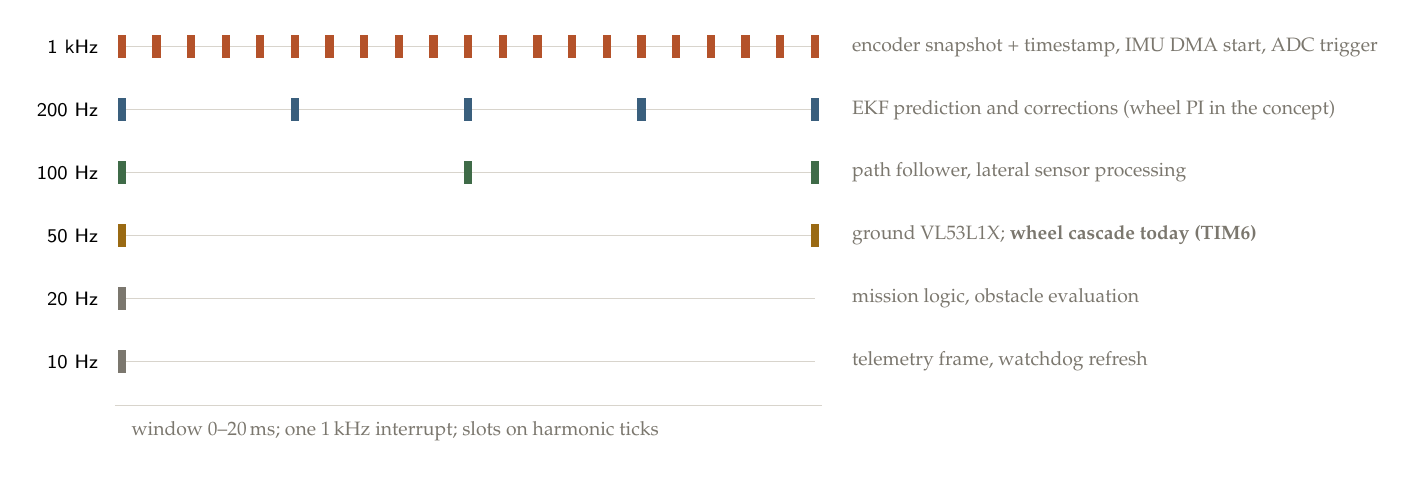
\begin{tikzpicture}[x=4.4mm,y=8.0mm]
  \foreach \lane/\name/\step/\col/\task in {
     0/{1 kHz}/1/accent/{encoder snapshot + timestamp, IMU DMA start, ADC trigger},
     1/{200 Hz}/5/cold/{EKF prediction and corrections (wheel PI in the concept)},
     2/{100 Hz}/10/good/{path follower, lateral sensor processing},
     3/{50 Hz}/20/warn/{ground VL53L1X; \textbf{wheel cascade today (TIM6)}},
     4/{20 Hz}/50/grey/{mission logic, obstacle evaluation},
     5/{10 Hz}/100/grey/{telemetry frame, watchdog refresh}}
  {
    \draw[rule,very thin] (0,-\lane) -- (20,-\lane);
    \node[anchor=east,font=\scriptsize\sffamily] at (-0.4,-\lane) {\name};
    \node[anchor=west,font=\scriptsize\color{grey}] at (20.8,-\lane) {\task};
    \foreach \i in {0,...,20} {
      \pgfmathtruncatemacro{\m}{mod(\i,\step)}
      \ifnum\m=0 \fill[\col] (\i-0.12,-\lane-0.18) rectangle ++(0.24,0.36); \fi
    }
  }
  \draw[rule] (-0.2,-5.7) -- (20.2,-5.7);
  \node[font=\scriptsize\color{grey},anchor=west] at (0,-6.1) {window 0--20\,ms; one 1\,kHz interrupt; slots on harmonic ticks};
\end{tikzpicture}
\caption{Target schedule. Every slot's execution time is measured with a GPIO
toggle and an oscilloscope --- the CPU load meter costs one pin.}
\end{figure}

\textbf{Today} the vehicle firmware runs the wheel cascade directly in the TIM6
interrupt at \qty{50}{Hz}; the main loop parses the two consoles. The transition
to the cyclic executive happens when the IMU and EKF arrive (week 8--10), with
the wheel cascade kept at 50\,Hz or moved to 200\,Hz together with an M/T speed
estimator (\cref{sec:opt}).

\textbf{Time base.} TIM2 free-running at \qty{1}{MHz} (32 bit, wraps after
\qty{71.6}{min}); every measurement is stamped from it at acquisition, not from
\code{HAL\_GetTick()} (\qty{1}{ms} resolution, interrupt-dependent). The
calibration firmware uses the DWT cycle counter for the same purpose and is
therefore independent of the TIM6 rate (tested at 50 and 83\,Hz with identical
results).

\subsection{Firmware components}

\begin{center}
\small
\begin{tabularx}{\textwidth}{@{}P{30mm}P{42mm}L@{}}
\toprule
\textbf{Firmware} & \textbf{Files} & \textbf{Content}\\
\midrule
Bench (week 5) & \code{bench\_config.h}, \code{motor}, \code{encoder}, \code{bench} & open-loop drivetrain, console, test sequences 0--6 (truth table, sign, deadband, $K_v$ sweep, demos, hand-turn)\\
Vehicle (teammate, extended) & \code{main.c} (USER CODE blocks) & BTS7960, encoders, trapezoid + P + FF/PI cascade, L/R sync, \code{D<mm>}, HC-12 console\\
Calibration & \code{calib.c/.h}, \code{calib\_config.h}, \code{calib\_host.py}, \code{sim/} & sign, breakaway, sweeps, backlash, ground sweep, odometry runs (\code{D}, \code{W}, \code{Q}); selected by \code{APP\_CALIB}; verified in software-in-the-loop simulation; 21--30\,KB\\
\bottomrule
\end{tabularx}
\end{center}

Module prefixes for the full firmware: \code{mot\_}, \code{enc\_}, \code{imu\_},
\code{vl\_}, \code{ekf\_}, \code{nav\_}, \code{msn\_}, \code{com\_}, \code{sys\_}; units in
identifiers (\code{\_mm}, \code{\_mms}, \code{\_rad}).

\subsection{Language and build rules}

\begin{itemize}[leftmargin=6mm]
\item C (not C++). Single precision only: every literal has \code{f}, no
\code{double}, \code{-Wdouble-promotion} on (it is missing in the current project
--- O-11), \code{-ffast-math} forbidden (it changes IEEE semantics the EKF relies
on). Console formatting with integers only.
\item Development at \code{-Og} (current project: \code{-O0}, O-11); the full
competition build at \code{-O2} in week 13, not 16 --- every missing
\code{volatile} surfaces on that day.
\item Flash budget: 60--90\,KB of 512\,KB expected; VL53L1X Ultra Lite Driver
($<\qty{10}{KB}$) instead of the full API ($\approx\qty{90}{KB}$);
\code{-Wl,--print-memory-usage} after every build.
\end{itemize}

\subsection{CubeMX regeneration protocol}

CubeMX owns the \code{.ioc}; code lives only in USER CODE blocks. Before every
regeneration: commit. After: \code{git diff} of \code{main.c} and \code{.cproject}.
CubeMX is known to reset values silently (TIM6 period, build flags). The clock
tree (PLLM = 4, HSE BYPASS) and TIM6 period are checked in the generated code
every time. Pins are reserved in \code{TOOLCHAIN.md} before they are touched in
CubeMX (USART1 on PB6/PB7 must be assigned before TIM1 CH2/CH3, or CubeMX places
it on PA9/PA10).
% =====================================================================
\clearpage
\section{Error budget and expected accuracy}\label{sec:budget}

Worked example: a \qty{40}{m} segment without external reference before a
waypoint, driven at \qty{0.4}{m/s} (\qty{100}{s}). Each term is computed with
the model of \cref{sec:odoerr,sec:imumodel,sec:tofmodel}.

\begin{center}
\small
\begin{tabularx}{\textwidth}{@{}P{42mm}P{44mm}P{24mm}L@{}}
\toprule
\textbf{Term} & \textbf{Assumption} & \textbf{Error at 40\,m} & \textbf{Model}\\
\midrule
Entry heading error & \ang{0.3} at segment start & \qty{21}{cm} lateral & $s\,\delta\psi_0$\\
\quad after a face fit & \ang{0.13} (VL53L1X, $\sigma_r=\qty{2}{cm}$, \qty{2}{m}, $N=250$) & \qty{8.8}{cm} lateral & \cref{eq:headingfit}\\
Residual gyro bias & \qty{1e-3}{\degree/s} after ZUPT & \qty{3.5}{cm} lateral & $\delta b\,s^2/(2v)$\\
Scale error & \qty{0.5}{\percent} & \qty{20}{cm} along & $\varepsilon_s s$\\
\quad after per-surface calibration & \qty{0.2}{\percent} (\code{D5000}$\times3$) & \qty{8}{cm} along & \\
\quad after a landmark fix near the waypoint & $\sigma\approx\qty{3}{cm}$ & \qty{3}{cm} along & \\
Turn on a \ang{6} slope (avoidable) & integrated body rate & \qty{35}{cm} lateral & \cref{eq:euler}\\
Backlash, one reversal & 1--2\,mm and \ang{0.3}--\ang{0.5} per reversal & avoid reversals & \cref{sec:encoder}\\
Stop accuracy of the controller & $|e_x|<\qty{2}{mm}$ & \qty{0.2}{cm} & \\
\bottomrule
\end{tabularx}
\end{center}

\begin{figure}[htbp]
\centering
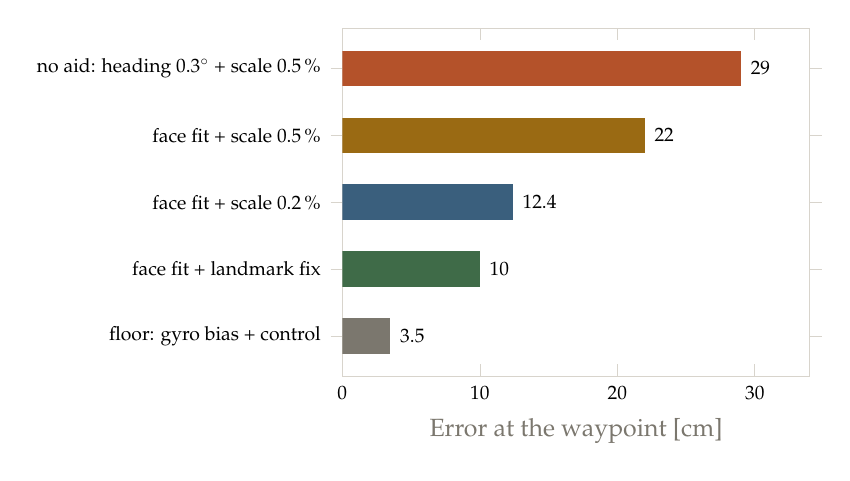
\begin{tikzpicture}
\begin{axis}[mr,
  width=0.62\textwidth, height=60mm,
  xbar, xmin=0, xmax=34,
  xlabel={Error at the waypoint [cm]},
  ymin=0.4, ymax=5.6, ytick={1,2,3,4,5}, y dir=reverse,
  yticklabels={{no aid: heading \ang{0.3} + scale 0.5\,\%},
               {face fit + scale 0.5\,\%},
               {face fit + scale 0.2\,\%},
               {face fit + landmark fix},
               {floor: gyro bias + control}},
  yticklabel style={font=\scriptsize,align=right},
  nodes near coords, nodes near coords style={font=\scriptsize},
  bar width=4.5mm, grid=none, every axis plot/.append style={bar shift=0pt},
]
\addplot[fill=accent,draw=none] coordinates {(29,1)};
\addplot[fill=warn,draw=none]   coordinates {(22,2)};
\addplot[fill=cold,draw=none]   coordinates {(12.4,3)};
\addplot[fill=good,draw=none]   coordinates {(10,4)};
\addplot[fill=grey,draw=none]   coordinates {(3.5,5)};
\end{axis}
\end{tikzpicture}
\caption{Root-sum-square of lateral and along-track terms (first bar
$\sqrt{21^2+20^2+3.5^2}=\qty{29}{cm}$). \textbf{The entry heading
dominates the lateral error and the scale dominates the along-track error.} One
face fit and one per-surface scale calibration move the waypoint into the
\qtyrange{10}{20}{cm} bracket (1.5 points); a landmark fix shortly before the
waypoint reaches the 1.75 boundary. The \qtyrange{0}{5}{cm} bracket needs both
fixes \emph{and} short reference-free stretches.}
\label{fig:budget}
\end{figure}

\begin{figure}[htbp]
\centering
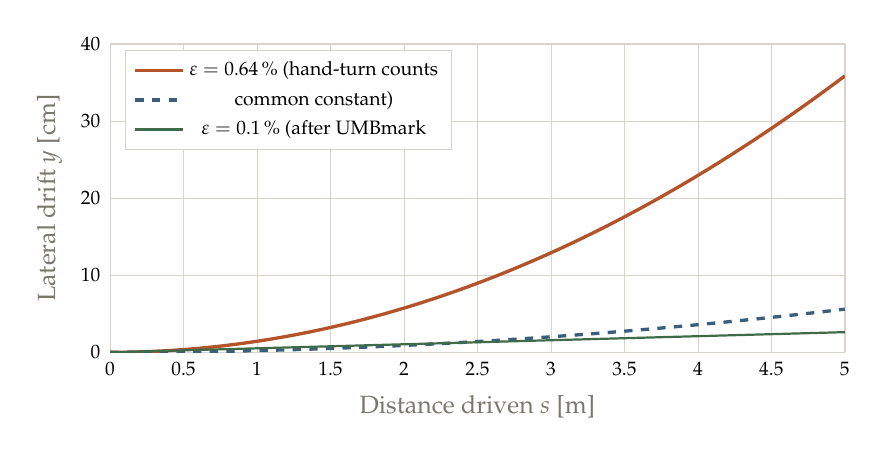
\begin{tikzpicture}
\begin{axis}[mr,
  width=0.9\textwidth, height=55mm,
  xlabel={Distance driven $s$ [m]}, ylabel={Lateral drift $y$ [cm]},
  xmin=0, xmax=5, ymin=0, ymax=40,
  legend style={at={(0.02,0.98)},anchor=north west},
]
  \addplot[accent,very thick,domain=0:5,samples=60]{100*0.0064*x^2/(2*0.22325)};
  \addplot[cold,very thick,dashed,domain=0:5,samples=60]{100*0.001*x^2/(2*0.22325)};
  \addplot[good,thick,domain=0:5,samples=2]{100*x*0.005236};
  \legend{$\varepsilon=0.64\,\%$ (hand-turn counts, common constant),
          $\varepsilon=0.1\,\%$ (after UMBmark, target),
          heading offset \ang{0.3} (linear)}
\end{axis}
\end{tikzpicture}
\caption{Encoder-only straight driving: a wheel-scale mismatch grows
quadratically (\cref{eq:drift}), a heading offset linearly. This is the
behaviour of today's firmware (no gyro); with gyro heading the quadratic term
leaves the estimate but remains in the L/R synchronisation.}
\label{fig:drift}
\end{figure}

\begin{keybox}
\textbf{Target and its justification.} Every waypoint inside
\qtyrange{10}{20}{cm} with a completed circuit. The two cheapest levers are the
survey (landmarks and faces near each waypoint) and per-surface scale
calibration; neither needs new hardware.
\end{keybox}

% =====================================================================
\section{Calibration and verification plan}\label{sec:calib}

\subsection{Calibration procedure (calibration firmware)}

\begin{enumerate}[leftmargin=6mm,label=\arabic*.]
\setcounter{enumi}{-1}
\item \textbf{Preparation.} Tyres clean, battery charged and mounted where it
rides on the course (load distribution changes the rolling radius), battery
voltage at the driver input measured and entered (\code{U11.92}).
\item \textbf{Stand, \code{A}} ($\approx\qty{7}{min}$): sign check, breakaway and
stop duty ($6\times$ per direction), descending duty sweep (16 levels,
$2\times$) giving $K_v$, $K_s$ per wheel and direction with standard errors,
$R^2$, residuals and $\tau$ at every level change. Optionally at full and at low
pack voltage.
\item \textbf{Backlash, \code{L}} (vehicle on the box, each tyre held by hand in
turn): lost motion with and without torque.
\item \textbf{Ground, \code{G}} ($\approx\qty{1.2}{m}$ of floor): closed-loop sweep at
8 speeds forward and back --- $K_v$, $K_s$ \textbf{under load}, the values for the
vehicle firmware.
\item \textbf{Odometry} on course-type paving:
(a) scale: \code{D5000} $\times3$ per surface, distance measured with tape;
(b) UMBmark: \code{Q2000} $\times5$ and \code{Q-2000} $\times5$, each preceded by
\code{D50} (gearboxes loaded forward) and marking the start;
(c) optional wheelbase check \code{W3600}/\code{W-3600} (10 turns);
(d) \code{odo} computes new mm/count L/R and wheelbase; enter with \code{O\ldots},
repeat two squares each way --- the return error should fall to a few millimetres.
\end{enumerate}

\textbf{Pose measurement.} Two pointers on the centre line, one ahead of
($p_f=\qty{150}{mm}$) and one behind ($p_r=\qty{100}{mm}$) the axle; mark both on
masking tape before and after a run, measure each displacement along and across
the start axis with a carpenter's square. The two points give axle position and
true heading change; errors are always \emph{real minus encoder}, so the result
does not depend on the controller.

\subsection{UMBmark}\label{sec:umbmark}

Borenstein's UMBmark drives an $L\times L$ square clockwise and
counter-clockwise; the centres of gravity of the return errors
$x_{cw},x_{ccw}$ separate the two systematic errors:
\begin{equation}
\alpha=\frac{x_{cw}+x_{ccw}}{-4L},\quad
\beta=\frac{x_{cw}-x_{ccw}}{-4L},\quad
R=\frac{L/2}{\sin(\beta/2)},\quad
E_d=\frac{R+b/2}{R-b/2},\quad
E_b=\frac{\pi/2}{\pi/2-\alpha},
\end{equation}
($\alpha,\beta$ in rad, signs per Borenstein's convention), corrected by
$b'=E_b\,b$, $D_L'=\tfrac{2}{E_d+1}D$, $D_R'=\tfrac{2}{1/E_d+1}D$. The calibration
script does not use these small-angle closed forms but fits $E_d$ and $E_b$ with
an exact arc model of the commanded square (Gauss--Newton over both directions
and both coordinates); in simulation with known truth the return error fell from
\qtyrange{250}{400}{mm} to below \qty{1}{mm}. UMBmark does not see the mean scale
--- hence step (a) first.

\subsection{Verification by layer}

\begin{center}
\small
\begin{tabularx}{\textwidth}{@{}lLl@{}}
\toprule
\textbf{Layer} & \textbf{Acceptance test} & \textbf{State}\\
\midrule
Actuation & signs (\code{C}), no forbidden state, enables low in reset & \tg{passed}\\
Speed loop & step 0$\to$200\,mm/s on the floor: overshoot $<5\,\%$, no stick-slip at \qty{0.1}{m/s} & \tw{to repeat on floor}\\
Position loop & \code{D300}, \code{D1000}, \code{D5000}: end within \qty{2}{mm} (encoder), no reversal, L/R difference $<\qty{3}{mm}$ & \tw{D1000 passed}\\
Odometry & UMBmark return error $<\qty{10}{mm}$ for $L=\qty{2}{m}$ & \tk{open}\\
IMU & Allan variance; bias vs temperature over \qty{20}{K} & \tk{after selection}\\
EKF stationary & bias converges in INIT; $P$ stays symmetric/positive & \tk{week 10}\\
EKF hand-pushed & \qty{10}{m} straight: estimate within \qty{10}{cm} & \tk{week 10}\\
Ground sensors & classify path/edging/grass on site, noon and afternoon & \tk{after fitting}\\
Path follower & closes a \qtyproduct{10x10}{m} rectangle within \qty{30}{cm} & \tk{week 13}\\
Mission & full circuit, waypoints within \qty{40}{cm} (wk 15), \qty{20}{cm} (wk 16) & \tk{weeks 15--16}\\
Radio & 15\,min logging at 10\,Hz, $<1\,\%$ lost frames; failsafe on link loss & \tk{weeks 10/14}\\
\bottomrule
\end{tabularx}
\end{center}
% =====================================================================
\clearpage
\section{Open items, missing values and optimisation}\label{sec:open}

Everything that is not yet measured, decided, implemented or verified is listed
here once, with the sections it blocks. Priorities: \tb{blocking},
\tw{high}, \tk{medium}, low.

\subsection{Field measurements --- nothing measured yet}\label{sec:open-field}

\begin{center}
\small
\begin{tabularx}{\textwidth}{@{}cP{62mm}Ll@{}}
\toprule
\# & \textbf{Measurement} & \textbf{Blocks} & \textbf{Prio}\\
\midrule
F-1 & Ramp-lip height & wheel and caster diameter (\cref{sec:longdyn}) & \tb{blocking}\\
F-2 & Ramp gradient & motor margin, whether slope projection is mandatory & \tw{high}\\
F-3 & Sidewalk width at the ramp entry & turning on level ground (\cref{sec:planning}) & \tw{high}\\
F-4 & Rubber-edging height, constancy, flush or proud & ground-sensor thresholds & \tw{high}\\
F-5 & Narrowest path width & maximum vehicle width & \tw{high}\\
F-6 & Residual width in furniture zones & whether evasion is possible there & \tk{medium}\\
F-7 & \textbf{Length of reference-free stretches, especially before each waypoint} & error budget --- the single most important number & \tb{blocking}\\
F-8 & Benches/tables: position $\pm\qty{5}{cm}$, face orientation $\pm\ang{0.5}$ & heading fits, landmark map & \tb{blocking}\\
F-9 & Posts: position and diameter & landmark map & \tw{high}\\
F-10 & Waste bins and other second-class landmarks & landmark map & \tk{medium}\\
F-11 & Total circuit length, leg lengths & time budget, path definition & \tw{high}\\
F-12 & Leg headings & path definition & \tw{high}\\
F-13 & Step: height, position, whether it is crossed anywhere & ground sensors, safety & \tw{high}\\
F-14 & Surface types per leg (paving, concrete, edging) & per-surface scale calibration & \tk{medium}\\
F-15 & Radio coverage along the course & heartbeat timeouts & low\\
\bottomrule
\end{tabularx}
\end{center}

Method: tape measure and carpenter's square for widths and heights; a
\qty{30}{m} tape and pairwise distances (trilateration) between fixed points for
the landmark map; photographs of every landmark from the path with a scale.
One afternoon unblocks F-1 to F-14.

\subsection{Vehicle parameters still to determine}\label{sec:open-params}

\begin{center}
\small
\begin{tabularx}{\textwidth}{@{}P{55mm}P{27mm}lL@{}}
\toprule
\textbf{Parameter} & \textbf{Current value} & \textbf{Status} & \textbf{How}\\
\midrule
Vehicle mass $m$, load split axle/casters & --- & \MEASURE & scale under each wheel\\
$K_v$, $K_s$ under load, per wheel and direction & bench / wheels-in-air & \MEASURE & \code{G}\\
Breakaway $K_{s,break}$ on BTS7960 & 14.1/16.9\,\% (bench) & \MEASURE & \code{B}\\
Plant time constant on the floor & 50\,ms (in air) & \MEASURE & \code{G}, steps\\
Driver output floor $U_{min}$ at 20\,kHz & --- & \MEASURE & oscilloscope\\
Armature $L_a$, $R_a$; $k_e$ & estimates only & \VERIFY & LCR meter, locked-rotor test\\
Mean scale $D/C$ per surface & 72.6\,mm/3584 & \VERIFY & \code{D5000}$\times3$\\
Per-wheel mm/count ($E_d$) & equal & \MEASURE & UMBmark\\
Effective wheelbase ($E_b$) & 223.25\,mm geometric & \MEASURE & UMBmark, \code{W$\pm$3600}\\
Backlash $\delta_b$ per wheel & --- & \MEASURE & \code{L}\\
Battery divider ratio & 5.7 nominal & \MEASURE & multimeter vs ADC\\
Session current / energy & --- & \MEASURE & log $U_{bat}$, coulomb count\\
Gyro: ARW, bias instability, temperature coefficient & --- & \MEASURE & Allan variance, temperature run\\
VL53L1X: $\sigma_r$ outdoors, class thresholds, max range in sun & --- & \MEASURE & outdoor afternoon\\
EKF noise: $k_d$, $q_b$, $q_s$, $R$ per measurement & --- & \MEASURE & from the above\\
Path-follower gains $\omega_n$, $\zeta$ & design 1.5--2\,rad/s, 0.7 & \VERIFY & rectangle test\\
Sync gain $K_{sync}$ & 3\,(mm/s)/mm & \VERIFY & L/R difference on \code{D5000}\\
\bottomrule
\end{tabularx}
\end{center}

\subsection{Firmware and configuration items}\label{sec:open-fw}

Numbering follows the sheet ``Offene Punkte'' of the CubeMX workbook.

\begin{center}
\small
\begin{tabularx}{\textwidth}{@{}cP{40mm}Ll@{}}
\toprule
\# & \textbf{Item} & \textbf{Why / how} & \textbf{Prio}\\
\midrule
O-1 & TIM6 period 199 & 119 gives 83\,Hz against \code{CTRL\_PERIOD\_S}\,=\,0.02; add a start-up printout of the measured rate & \tb{blocking}\\
O-2 & End of move with $K_s$ intercept & wheel may stop short (static friction); breakaway switching or higher $K_i$; verify \code{D300}/\code{D1000} within 2\,mm & \tw{high}\\
O-3 & Battery operation without USB & HSE BYPASS depends on ST-Link MCO (\cref{sec:clock}); fallback crystal at X3 & \tw{high}\\
O-4 & Hot AMS1117 & measure its input, supply HC-12 separately & \tw{high}\\
O-5 & \code{V\_NOM\_MAX} 800 $\to$ 500 & drive saturates above $\approx\qty{650}{mm/s}$ & \tk{medium}\\
O-6 & \code{EVT\_TIMEOUT} & settle timeout currently reports DONE & \tk{medium}\\
O-7 & Per-wheel mm/count & L/R from UMBmark; raise $D$ to $\approx\qty{73.0}{mm}$ if per-wheel counts are used & \tk{medium}\\
O-8 & Straight-line drift & \code{D1000/2000/4000} lateral offset (shape tells the cause) & \tk{medium}\\
O-9 & Speed limit under load & \code{D3000} at 300--500\,mm/s, full and empty pack; 80\,\% of the first failing speed & \tk{medium}\\
O-10 & HSE start-up timeout 1000\,ms & RCC parameter; avoids failed start at power-on & \tk{medium}\\
O-11 & Build flags & \code{-Og}, \code{-Wdouble-promotion}; \code{git diff .cproject} after regeneration & \tk{medium}\\
O-12 & Error\_Handler stops motors & \code{GPIOB->BSRR = (PIN12|PIN13)<<16}, CCR1--4 = 0 & \tw{high}\\
O-13 & HC-12 channel coordination & all teams start on CH001 & \tk{medium}\\
O-14 & $K_v$ sweep on the BTS7960 & superseded by calibration \code{A}/\code{G} & low\\
O-15 & PB7 pull-up, PH1 free & check \code{HAL\_UART\_MspInit}, pinout view & low\\
O-16 & CSS with callback & EN\_L/EN\_R low on clock failure & later\\
O-17 & TIM2 as 1\,MHz time base & PSC 89, start base + IC & week 8\\
O-18 & SPI1, I2C1/2, ADC1, DMA, IWDG & sensor bring-up & week 8+\\
O-19 & Confirm which build is flashed & PI gains 0.10/0.50 vs SIMC 0.045/0.898; KS\_BREAK switching & \tw{high}\\
O-20 & Replacement Nucleo & board failure reported 10 Oct; re-verify clock tree on the new board & \tb{blocking}\\
\bottomrule
\end{tabularx}
\end{center}

\subsection{Decisions}\label{sec:open-decisions}

\begin{center}
\small
\begin{tabularx}{\textwidth}{@{}cP{40mm}Ll@{}}
\toprule
\# & \textbf{Decision} & \textbf{Options and recommendation} & \textbf{Blocks}\\
\midrule
D-1 & IMU & ISM330DHCX (Adafruit) --- decided & week-8 milestone\\
D-2 & Radio & keep HC-12 / XBee 3 Pro (certified, own MCU) & week 10/14\\
D-3 & Caster type and size & after F-1 & chassis\\
D-4 & Ground-sensor mounting height and offsets & 100--200\,mm, offsets 15/25\,cm & spot size, thresholds\\
D-5 & HC-12 supply & 5\,V branch (recommended) or second LDO & O-4\\
D-6 & Hardware E-stop in series with EN & recommended, firmware-independent & safety\\
D-7 & PWM frequency & keep 20\,kHz unless $U_{min}$ is large & low-speed resolution\\
D-8 & Wheel loop rate & 50\,Hz now; 200\,Hz only with an M/T estimator & path bandwidth\\
D-9 & Start-heading jig & physical alignment of $\{W\}$ & EKF init\\
D-10 & Spare parts & Nucleo, BTS7960, motor & schedule risk\\
D-11 & Second battery & decided; order & 3-h sessions\\
\bottomrule
\end{tabularx}
\end{center}

\subsection{Questions}\label{sec:open-questions}

\begin{center}
\small
\begin{tabularx}{\textwidth}{@{}cLP{24mm}l@{}}
\toprule
\# & \textbf{Question} & \textbf{To} & \textbf{Urgency}\\
\midrule
Q-1 & Is 3.4\,kgf\,cm the rated or the stall torque? (model says rated) & vendor & low\\
Q-2 & Restock lead time HS5141-178 (spare) & vendor & medium\\
Q-5 & Do two driven wheels plus two casters satisfy ``four-wheeled''? & professor & \tb{highest}\\
Q-6 & How many vehicles on the course simultaneously? & professor & high\\
Q-7 & Furniture in the same place on exam day? & professor & high\\
Q-8 & Legal radio band in Mexico for the link & IFT / professor & high\\
Q-9 & HC-12 FU mode and over-the-air rate & datasheet & low\\
Q-10 & Are radio modules and ToF sensors with their own firmware acceptable under ``only STM32''? & professor & high\\
Q-11 & May the PC receive telemetry during graded AUTO runs? & professor & medium\\
Q-12 & How is waypoint accuracy aggregated (per waypoint, mean, worst)? & professor & medium\\
\bottomrule
\end{tabularx}
\end{center}
(Q-3 connector pinout and Q-4 driver truth table are answered; \cref{sec:bench}.)

\subsection{Risk register}

\begin{center}
\small
\begin{tabularx}{\textwidth}{@{}LLL@{}}
\toprule
\textbf{Risk} & \textbf{Impact} & \textbf{Mitigation}\\
\midrule
Course not surveyed in time & wheel size, landmarks, budget all unknown & one afternoon, now (F-1\ldots F-14)\\
No spare parts & a failure costs a week (already happened once) & D-10\\
IMU not delivered by week 8 & milestone and all heading aiding late & order the ISM330DHCX now; placeholder IMU for bring-up\\
Clock without USB fails & no autonomous run on battery & O-3: test, power bank, crystal\\
CubeMX regeneration reverts values & wrong tick rate, lost flags; ``mysterious'' behaviour & commit, \code{git diff}, start-up rate printout\\
Turn on a slope & 35--62\,cm cross-track error from one manoeuvre & turn on level ground, slope projection\\
Ground sensors in sun & missed edge $\Rightarrow$ grass $\Rightarrow$ invalid run & thresholds tested at noon; inner interlock\\
Other robots' ToF/radio & phantom ranges, collisions on CH001 & median + gate + signal check; frame IDs + CRC; channel plan\\
Single TX buffer race & corrupted frames that look like noise & double buffering (done in bench firmware)\\
Safety rule vs measurement & supervisor aborts its own test & scope stall checks per mode\\
Motor pairing (12\,\%/20\,\%) & arcs in open loop & per-wheel FF + PI + sync (done)\\
Dupont on motor leads & heat, drifting series resistance & crimped/soldered $\ge$20\,AWG before driving\\
Regulatory status of 433\,MHz & module unusable officially & D-2, Q-8\\
\bottomrule
\end{tabularx}
\end{center}

% ---------------------------------------------------------------------
\subsection{Optimisation roadmap}\label{sec:opt}

Ordered by expected points per effort. Items 1--5 need no new hardware.

\begin{enumerate}[leftmargin=7mm]
\item \textbf{Survey the course} (F-1\ldots F-14). Unblocks everything below
and defines where the heading fits and landmark fixes come from.
\item \textbf{Per-surface scale and UMBmark.} Per-wheel mm/count, effective
wheelbase, and backlash as a per-wheel dead band in odometry (first
$\delta_b$ counts after a reversal do not move the wheel). Expected: return error
of a 2-m square from centimetres to millimetres; along-track scale to
\qty{0.2}{\percent}.
\item \textbf{Battery-normalised feedforward.} Fit the feedforward in volts
($K_v^V$, $K_s^V$ with $U_{bat}$ recorded), measure $U_{bat}$ on PA0 at
\qty{20}{Hz} with a low-pass, apply $d_{ff}=(\ldots)/U_{bat}$. Removes a
\qty{27}{\percent} gain variation over the discharge from the PI's job.
\item \textbf{Ground-identified constants} from \code{G} and \code{B}; the
breakaway switching with measured values; inertia feedforward with the floor
$\tau_m$.
\item \textbf{Better low-speed speed estimate (M/T method).} Sample the encoder
counter with a \qty{1}{\micro s} timestamp at \qty{1}{kHz} and compute speed over
the interval between the first and last \emph{count change} inside a window,
$\hat v=c\,\Delta n/\Delta t_{edges}$. Resolution then improves from
\qty{3.18}{mm/s} to well below \qty{1}{mm/s} at approach speeds, the IIR filter
(\qty{29}{ms} lag) can be lighter, $\theta$ shrinks, and SIMC allows a faster
speed loop --- which in turn allows a faster position and path loop.
\item \textbf{Grade feedforward.} With pitch $\vartheta$ from the IMU, add the
duty that holds the vehicle on the slope,
$\Delta d\approx\frac{R_a}{k_t U_{bat}}\cdot\frac{m g\sin\vartheta\,r}{2\,i\,\eta}$,
identified directly as $\Delta d/\sin\vartheta$ from a ramp test. The PI then
does not have to wind up on the ramp.
\item \textbf{ZUPT at every stop}, not only at waypoints --- in particular
before every turn (fresh bias immediately before the manoeuvre that converts
heading error into cross-track error).
\item \textbf{Gyro temperature model} from a warm-up run; 10-minute warm-up before
graded runs.
\item \textbf{Heading fits at every straight face} before reference-free
stretches, and a landmark fix within a few metres of each waypoint (\cref{fig:budget}).
\item \textbf{Path-follower gain scheduling} ($k_y=\omega_n^2/v$) and curvature
feedforward on ARC segments; saturation that keeps $\omega$ and reduces $v$.
\item \textbf{Offline optimisation from practice runs.} Log full-rate data with
\code{CAPTURE}; re-estimate scale, wheelbase, sensor offsets and the landmark map
by smoothing the recorded runs; burn the constants in (week 15).
\item \textbf{Safety hardening:} hardware E-stop in the EN lines, IWDG, CSS with
motor stop, Error\_Handler that stops the motors.
\item \textbf{Mechanics:} hard, narrow tyres (stable rolling radius, defined
contact point and therefore defined $b$); IMU rigidly at the axle midpoint;
battery fixed where it rides during calibration.
\end{enumerate}

\begin{keybox}
\textbf{Next five actions.} (1) Fix TIM6 = 199 and confirm the flashed build
(O-1, O-19) on the replacement board (O-20). (2) Survey the course (F-1\ldots
F-14). (3) Run calibration \code{A}, \code{L}, \code{G} and the odometry sequence.
(4) Order the IMU (D-1, ISM330DHCX); the five VL53L1X are ordered. (5) Ask the professor Q-5, Q-7, Q-10.
\end{keybox}
% =====================================================================
\clearpage
\appendix
\section{Constants register}\label{app:constants}

All numerical constants of the vehicle firmware (\code{main.c}, USER CODE PD) and
the physical constants used in this document. \emph{Source:} M = measured,
C = catalogue, D = design value, E = estimate.

{\footnotesize
\begin{xltabular}{\textwidth}{@{}P{55mm}P{30mm}P{17mm}cL@{}}
\toprule
\textbf{Constant} & \textbf{Value} & \textbf{Unit} & \textbf{Src} & \textbf{Note}\\
\midrule
\endfirsthead
\toprule
\textbf{Constant} & \textbf{Value} & \textbf{Unit} & \textbf{Src} & \textbf{Note}\\
\midrule
\endhead
\bottomrule
\endfoot
\multicolumn{5}{@{}l}{\textbf{\textsf{Mechanics and odometry}}}\\
\code{WHEEL\_DIAMETER\_MM} & 72.6 & mm & M & effective, valid with $C=3584$\\
\code{COUNTS\_PER\_WHEEL\_REV} & 3584 & counts & D & $64\times56$; measured 3595/3618\\
\code{MM\_PER\_COUNT} & 0.063638 & mm & M & ratio $\pi D/C$\\
\code{MM\_PER\_COUNT\_L/R} & $\times1.0000$ & --- & D & per-wheel factors, from UMBmark\\
\code{WHEEL\_BASE\_MM} & 223.25 & mm & M & geometric; effective from UMBmark\\
\midrule
\multicolumn{5}{@{}l}{\textbf{\textsf{Signs and actuation}}}\\
\code{ENC\_L\_SIGN / ENC\_R\_SIGN} & $+1$ / $-1$ & --- & M & vehicle harness\\
\code{MOT\_L\_SIGN / MOT\_R\_SIGN} & $-1$ / $+1$ & --- & M & positive duty $\Rightarrow$ forward\\
\code{PWM\_FREQ\_HZ} & 20000 & Hz & D & TIM1 ARR 8999\\
\midrule
\multicolumn{5}{@{}l}{\textbf{\textsf{Control loop}}}\\
\code{CTRL\_PERIOD\_S} & 0.02 & s & D & must equal the TIM6 period (199)\\
\code{SPEED\_FILTER\_ALPHA} & 0.5 & --- & D & IIR, $\tau_f=\qty{29}{ms}$\\
\code{KV\_L / KV\_R} & 0.00492 / 0.00507 & duty/rpm & M & bench\\
\code{KS\_L / KS\_R} & 0.110 / 0.127 & duty & M & bench intercepts\\
\code{FF\_KS\_L/R\_PCT} & 9.8 / 4.1 & \% & M & BTS7960 in air (revised build)\\
\code{FF\_KV\_L/R} & 0.1275 / 0.1361 & \%/(mm/s) & M & BTS7960 in air (revised build)\\
\code{KS\_BREAK\_L/R\_PCT} & 14.1 / 16.9 & \% & M & bench breakaway; replace by \code{B}\\
\code{TAU\_PLANT\_S} & 0.050 & s & M & inertia feedforward\\
\code{V\_MOVING / V\_STOPPED / V\_ZERO} & 8 / 3 / 2 & mm/s & D & friction switching, zero command\\
\code{KICK\_DUTY\_PCT / KICK\_TICKS} & 40 / 5 & \%, ticks & D & superseded by breakaway switching\\
\code{KP\_SPEED / KI\_SPEED} & 0.10 / 0.50 $\to$ 0.045 / 0.898 & \%/(mm/s), /s & D & SIMC balanced\\
\code{INTEG\_MAX\_PCT} & 30 & \% & D & anti-windup\\
\code{KP\_POS} & 2 & (mm/s)/mm & D & $\tau=\qty{0.5}{s}$\\
\code{V\_CORR\_MAX\_MM\_S} & 100 & mm/s & D & position-loop clamp\\
$K_{sync}$ (\code{Y}) & 3.0 & (mm/s)/mm & D & L/R synchronisation\\
\code{SETTLE\_V\_MM\_S / POS\_TOL\_MM} & 20 / 2 & mm/s, mm & D & end of move\\
\code{SETTLE\_TICKS / FAULT\_TICKS} & 50 / 30 & ticks & D & 1\,s / 0.6\,s\\
\midrule
\multicolumn{5}{@{}l}{\textbf{\textsf{Limits and interface}}}\\
\code{V\_NOM\_DEFAULT / V\_NOM\_MAX} & 300 / 800 & mm/s & D & max to 500 (O-5)\\
\code{ACC\_MS / DEC\_MS\_DEFAULT} & 1000 / 1000 & ms & D & 0.3\,m/s$^2$ at 300\,mm/s\\
\code{MIN / MAX\_DIST\_MM} & 5 / 20000 & mm & D & \\
\code{DEADMAN\_MS} & 2000 & ms & D & open loop only\\
\code{AUTO\_PRINT\_MS} & 250 & ms & D & \\
\code{RX\_LINE\_MAX} & 16 & chars & D & \\
\midrule
\multicolumn{5}{@{}l}{\textbf{\textsf{Physical and electrical}}}\\
Gear ratio & 56.3 & --- & C & implied 56.17 / 56.53 (hand-turn)\\
Counts per motor revolution & 64 & --- & M & 16 PPR $\times4$\\
No-load speed & 181 / 177 & rpm & M & bench, $d=1$\\
Stall current & 4.3 & A & C & per motor\\
Rated torque & 3.4 & kgf\,cm & C & rated vs stall: Q-1\\
$k_e$, $R_a$ & 10.0\,mV\,s/rad, 2.8\,$\Omega$ & --- & E & \cref{sec:motor}\\
Plant $K$, $\tau_m$, $u_0$ & 7.596, 50\,ms, 7.0\,\% & --- & M & BTS7960, in air\\
Battery & 9.9--12.6 & V & C & 3S, 2.2\,Ah, 35C\\
Cut-off & 10.0 & V & D & \\
Divider & 10/57 & --- & D & 47\,k$\Omega$/10\,k$\Omega$\\
Encoder pull-ups & $\approx3$ & k$\Omega$ & M & A--B 6\,k$\Omega$\\
Encoder filter & 2.84 & \textmu s & D & IC filter 15\\
\end{xltabular}
}

\section{Glossary}\label{app:glossary}

{\small
\begin{xltabular}{\textwidth}{@{}lL@{}}
\toprule
\textbf{Term} & \textbf{Meaning}\\
\midrule
\endfirsthead
\toprule
\textbf{Term} & \textbf{Meaning}\\
\midrule
\endhead
\bottomrule
\endfoot
ARR & auto-reload register of a timer: the counter period minus one\\
ARW & angle random walk: integrated white rate noise of a gyroscope, in $^\circ/\sqrt{\mathrm{h}}$\\
CCR & capture/compare register of a timer channel; sets the PWM duty\\
CKD & clock-division field of a timer; sets the digital-filter sampling clock $f_{DTS}$\\
COBS & consistent-overhead byte stuffing: framing that removes zero bytes so that 0 can delimit frames\\
CRC & cyclic redundancy check\\
CSS & clock security system: hardware fallback to HSI and NMI when the external clock fails\\
DMA & direct memory access: data transfer without CPU involvement\\
DRDY & data-ready output of a sensor\\
DWT & data watchpoint and trace unit; contains the CPU cycle counter\\
E5V & external \qty{5}{V} supply input of the Nucleo (CN7-6)\\
EKF & extended Kalman filter: Kalman filter on linearised non-linear models\\
FF & feedforward: control action computed from the model and the set-point, not from the error\\
HSE / HSI / LSI & high-speed external / high-speed internal / low-speed internal clock\\
ICR & instantaneous centre of rotation\\
IIR & infinite-impulse-response (recursive) filter\\
IWDG & independent watchdog (own LSI clock)\\
MCO & microcontroller clock output; here of the ST-Link MCU, used as HSE\\
M/T method & speed measurement combining a count (M) with a measured time between edges (T)\\
NHC & non-holonomic constraint: zero lateral velocity of a wheeled vehicle\\
PI & proportional-integral controller\\
PLL & phase-locked loop; multiplies the input clock to the system clock\\
PPR & pulses per revolution (per channel)\\
PWM & pulse-width modulation\\
ROI & region of interest: active SPAD sub-array of the VL53L1X\\
SIMC & Skogestad internal model control: analytic PI/PID tuning rules\\
SPAD & single-photon avalanche diode\\
ToF & time of flight\\
UMBmark & University of Michigan Benchmark: square-path test separating wheel-diameter and wheelbase errors\\
VCP & virtual COM port of the ST-Link\\
XSHUT & shutdown input of the VL53L1X, used for address assignment\\
ZUPT & zero-velocity update: using standstill as a measurement (here of the gyro bias)\\
\end{xltabular}
}

\section{References}\label{app:refs}

\begin{enumerate}[label={[\arabic*]},leftmargin=8mm,itemsep=2pt]
\small
\item Challenge brief \emph{Challenge MR2006B}, Tecnol\'ogico de Monterrey, 2026.
\item Project documents: \code{CONCEPT.md} (Rev.\,E) and \code{CONCEPT\_REV\_F\_CHANGES.md};
\code{BENCH\_README.md}; \code{CALIB\_README.md} (9 Oct 2026);
\code{MR2006B\_CubeMX\_Konfiguration.xlsx} (9 Oct 2026); \code{TOOLCHAIN.md};
\code{MR2006B\_Pinout.xlsx}.
\item STMicroelectronics, \emph{RM0390: STM32F446xx advanced Arm-based 32-bit MCUs ---
Reference manual}.
\item STMicroelectronics, \emph{UM1724: STM32 Nucleo-64 boards (MB1136) --- User manual}.
\item STMicroelectronics, \emph{STM32F446xC/E datasheet}.
\item Infineon, \emph{BTS7960 High Current PN Half Bridge --- Data sheet}.
\item STMicroelectronics, \emph{VL53L1X datasheet} and \emph{UM2510: VL53L1X ultra lite driver}.
\item Silicon Labs, \emph{Si4463 datasheet}; HC Information Technology, \emph{HC-12 wireless serial port communication module --- user manual}.
\item J.~Borenstein, L.~Feng, ``Measurement and correction of systematic odometry
errors in mobile robots,'' \emph{IEEE Trans.\ Robotics and Automation}, 12(6),
pp.\ 869--880, 1996.
\item S.~Skogestad, ``Simple analytic rules for model reduction and PID controller
tuning,'' \emph{Journal of Process Control}, 13(4), pp.\ 291--309, 2003.
\item S.~Thrun, W.~Burgard, D.~Fox, \emph{Probabilistic Robotics}, MIT Press, 2005.
\item R.~Siegwart, I.~Nourbakhsh, D.~Scaramuzza, \emph{Introduction to Autonomous
Mobile Robots}, 2nd ed., MIT Press, 2011.
\item R.~C.~Coulter, \emph{Implementation of the Pure Pursuit Path Tracking
Algorithm}, CMU-RI-TR-92-01, Carnegie Mellon University, 1992.
\item IEEE Std 952-1997, \emph{IEEE Standard Specification Format Guide and Test
Procedure for Single-Axis Interferometric Fiber Optic Gyros} (Allan variance
method).
\item M.~S.~Grewal, A.~P.~Andrews, \emph{Kalman Filtering: Theory and Practice
Using MATLAB}, Wiley (Joseph-form covariance update).
\end{enumerate}

\end{document}
